\documentclass[ugrad,lot,lof,openright,11pt,oneside,onehalfspace]{RUthesis}
\usepackage{ifthen}
\usepackage{xspace}
\usepackage{amsmath}
\usepackage{bbm}
\usepackage{SIunits}
\usepackage{hyperref}
\usepackage{listings}
\usepackage{float}
\usepackage{longtable}
\usepackage{graphicx}
\usepackage{array}
\usepackage{caption}
\usepackage{pdfpages}
\usepackage[titletoc]{appendix}

\DeclareMathOperator{\sgn}{sgn}
\DeclareMathOperator{\bx}{\text{\bf x}}
\DeclareMathOperator{\bX}{\text{\bf X}}
\DeclareMathOperator{\bY}{\text{\bf Y}}
\DeclareMathOperator{\Prob}{Prob}
\DeclareMathOperator{\bnu}{\text{\boldmath{$\nu$}}}

\newcommand{\be}{\begin{equation}}
\newcommand{\ee}{\end{equation}}
\newcommand{\ben}{\begin{equation*}}
\newcommand{\een}{\end{equation*}}
\newcommand{\bea}{\begin{eqnarray}}
\newcommand{\eea}{\end{eqnarray}}
\newcommand{\bean}{\begin{eqnarray*}}
\newcommand{\eean}{\end{eqnarray*}}
\newcommand{\dif}{\mathrm{d}}
\newcommand{\me}{\mathrm{e}}
\newcommand{\e}[1]{\ensuremath{\times10^{#1}}}

\addunit{\dpi}{dpi}
\addunit{\tcid}{TCID\ensuremath{_{50}}}

\title{Software for Multi-level Monte-Carlo Simulation of Stochastic Biochemical Kinetics}
\author{Dexter Barrows}
\RUdegree{Bachelor of Science}
\RUfield{Mathematics and its Applications}
\RUsupervisor{Dr.\ Silvana Ilie}
\RUdepartment{Mathematics}
\RUsubmitdate{April 28, 2014}
\RUaddress{Department of Mathematics,\\
    Ryerson University,\\
    Toronto, Ontario \\
    Canada \\
    M5B 2K3}
\RUyear{2014}


\RUdedication{~\\
			  my Mom\\
			  ~\\
			  without whom\\
			  nothing I achieve\\
			  would be possible}

\RUabstract{
	\noindent
	Stochastic models for systems of biochemical reactions are essential to the field of Systems Biology. While the Chemical Master Equation provides accurate predictions of future states of well-stirred biochemical systems, the solutions to this model are too analytically complex to obtain for realistic systems, and direct numerical methods are likewise too computationally complex to be a feasible solution. Thus, Monte Carlo-type methods such as the Stochastic Simulation Algorithm (SSA) are utilized by scientists to obtain results consistent with solutions to the Chemical Master Equation but with drastically reduced complexity. This thesis discusses our program for the simulation of stochastic models of well-stirred biochemical kinetics, the Modelling Arrays of Reaction Software (MARS). Among other simulation methods, we implemented a very recent and advanced numerical strategy to estimate the average behaviour of the biochemical system, the multilevel Monte Carlo (MLMC) tau-leaping method. We compared the predictions of the MLMC with those of the exact SSA. The results showed excellent agreement, with the multilevel Monte Carlo tau-leaping method demonstrating a greatly reduced running time.
	}

\RUacknowledgement{
	\noindent
	I have been very fortunate to have had great help, support, and education during my time at Ryerson. In particular, my supervisor, Dr.~Silvana Ilie, has been nothing short of exceptional. Her guidance, patience, and mentorship have had an enormous effect on me, one I have no doubt will be long lasting. I also want to thank my Mom and Dad, my friends, and my family for being so supportive over the years, and for generally putting up with me.
	}

\begin{document}

\maketitle

\chapter{Introduction}

	Chemical reactions form the basis for virtually all biological processes, and understanding them is crucial to the progress of scientific discovery. Single chemical reactions have long been studied, quantified, qualified, experimented upon, and been thoroughly understood by the scientific community. However, it is not a single chemical reaction that can serve as the basis for something as complex as a biological organism, but rather dynamic systems of reactions with overlapping species that cannot be unlinked. The chemical systems associated with biological processes are referred to as systems of biochemical reactions.\\
	\\
	Mathematical models of biochemical reaction systems provide valuable analytical tools that can be used to understand and predict the behaviour of such systems. These models aim to determine the evolution of dynamic populations of species over elapsing time. The building blocks of all such models are differential equations, which relate functions to their derivatives. They are used to construct two overarching types of models: ones which are continuous in time, and ones that take discrete values depending on time \cite{sys_bio_intro}. The classical approach to modelling chemical reactions uses the former approach, employing systems of differential equations. These models are also deterministic, meaning they do not take into account the ``noise'', or elements of randomness, present in actual systems of biochemical reactions. The prototypical model of this type is the Reaction Rate Equation (RRE) \cite{gillespie_review}. It has since been accepted that systems that do take noise into account are necessary in order to provide realistic results \cite{phage_bacteria},\cite{sys_bio_intro}. The stochastic models may be continuous or discrete.\\
	\\
	Fundamentally, all stochastic models work on the same idea: they do not provide exact deterministic behaviour of a system, but rather a probabilistic outcome. The finest model of well-stirred biochemical kinetics is the Chemical Master Equation (CME) \cite{cme_intro},\cite{gillespie_review}, a discrete and stochastic model. The solution to the CME, really a system of coupled ordinary differential equations (ODEs), is a probability distribution of potential systems states at a given future time. While a solution to the CME is the ideal way to represent systems of well-stirred biochemical reactions, this is not analytically or numerically possible for all but the simplest of systems -- the CME is too complex for these approaches. However, single, exact realizations of the CME can be numerically generated by the Stochastic Simulation Algorithm (SSA), due to Gillespie \cite{ssa_intro},\cite{gillespie_review}, which uses discrete species populations to probabilistically simulate a series of reactions at variable-size time steps. To reduce the computational complexity, these exact trajectories can be in turn approximated through the consolidation of multiple reactions in fixed-size intervals, known as the tau-leaping method, introduced by Gillespie in \cite{sim_chem_reactions}. A further reduction is possible when large populations are present. Then, the molecular numbers may be represented as continuous populations. The reduced stochastic continuous model is known as Chemical Langevin Equation (CLE) \cite{sim_chem_reactions}. Good approximations of the probability distribution provided by the solution to the CME can be obtained by generating a large number of independent trajectories using SSA, the tau-leaping, or the pathwise simulation of CLE, usually on the order of 10,000 trajectories. Often, the mean and standard deviation of the results constitute the quantities of interest for applications.\\
	\\
	This work will discuss the theoretical framework required for stochastic modelling of well-stirred systems of biochemical reactions, the derivation of the CME, SSA, tau-leaping, CLE, and RRE models, and present the conditions under which these modelling approaches and simulation methods are valid in Chapter 2. Chapter 3 will introduce an advanced method for generating linked trajectories that greatly reduce the computational complexity of the algorithm for the same accuracy, the multilevel Monte Carlo (MLMC) tau-Leaping \cite{mlmc_applications},\cite{mlmc_complexity}.\\
	\\
	Chapter 4 will describe and provide documentation for our program which implements all of the aforementioned methods, the Modelling Arrays of Reactions Software (MARS). MARS allows the user, through the simulation method of their choosing, to obtain or plot predictive data for the evolution in time of the species populations in a biochemical system contained in a Systems Biology Markup Language (SBML) file. It has two primary function modes: it can generate a single trajectory to display the general system behaviour, or can use on the order of 10,000 independent trajectories to predict the mean behaviour of the system. Additionally, Chapter 4 outlines the many optional user-specified options that MARS can accept, which contributes to making the implementation quite robust. Appendix A contains all original source code, as well as a link to a version of the code with the additional open-source libraries required for operation \cite{sbml_toolbox},\cite{libsbml}.\\
	\\
	Lastly, Chapter 5 will present numerical results obtained using MARS to simulate several systems of biochemical reactions. The SSA, tau-leaping, the numerical methods for the CLE, and RRE will be compared through simulation of the classic Michaelis-Menten system \cite{sim_chem_reactions}, and the Schl\"{o}gl model \cite{schlogl}. The MLMC method will be compared to SSA through the simulation of the Goldbeter-Koshland Switch, a cyclical reaction system, and a potassium channel model \cite{chem_phys_models}.

\chapter[Background]{Background}

	\section{Motivation for Stochastic Modelling of Biochemical Systems}

		Systems Biology at its core is the study of the complex interactions between components of organisms. Its goal is to describe the function and behaviour of all parts of a biological system, and in turn the organism as a whole. It is a broad field with many areas of study. One such area focuses on modelling interactions of populations of biochemical molecules. The field has evolved over the years to move beyond the study of single biomolecules into the interaction of many different types of these molecules engaged in reactions, the aim of which is to describe and eventually predict the system's behaviour.\\
		\\
		Originally, these dynamic systems have been modelled as sets of coupled ordinary differential equations (ODEs). This model is called the Reaction-Rate Equation (RRE). On a larger scale, this approach works quite well, but it is intrinsically ill-suited to describing systems at the cellular level where the number of molecules may be much, much smaller. As this model is continuous and deterministic, it is unable to take into account the ``noise'' in a system. In fact, it has been well-established that biochemical kinetics at a cellular level contain a natural degree of unpredictability or randomness (stochasticity), that makes accurate description of their behaviour simply beyond the grasp of the RRE. As such, it has become generally accepted that stochastic models are required in order to present a realistic mathematical model of cellular-level biochemical kinetics.\\
		\\
		However, problems arise. Chief among them is that these stochastic models are computationally very demanding. In order to reduce complexity, a key assumption must be made: cells (containers) must be treated as well-mixed, eliminating the concern over the spacial component of the system. This is not out of the ordinary, deterministic models make this assumption as well. Further, this approach gives accurate results while allowing the state of a system at a given point in time to be represented as a vector containing the number of each type of molecule present. Even with this assumption, only simple networks can be feasibly approached with standard tools. In this case, it is possible to generate a probability distribution of the state of the system over time. Models of more complexity, even ones as simple as consisting of more than single-molecule reactions, quickly become analytically intractable. It is important to note that any systems that would be of practical interest belong to this latter class. Then software tools are needed to numerically approximate the solution of the mathematical models of biological processes. Mathematically, the state of a system is modelled as a Markov process.

	\section{Modelling and Simulation of Biochemical Systems}

		\subsection{Stochastic Discrete Model}

			\subsubsection{Model: Chemical Master Equation}

				With the need for stochastic modelling established, we must then turn to the mechanics of constructing such a model. First, the mathematical representation of a biochemical systems must be formalized. As per the previous section, consider a thermally and spatially isolated container containing biochemical molecules which we will be treating as well-stirred. Let there be $N$ such species $\{S_1,\ldots,S_N\}$ that interact through a system of $M$ chemical reactions $\{R_1,\ldots,R_M\}$. The state of the system can then be represented such that the number of each individual type of molecule $S_i$ at a given time $t$ is denoted $X_i(t)$, with the so-called state vector of the system being represented as $\mathbf{X}(t) \equiv (X_{1}(t),\ldots,X_{N}(t))$. We also assume that the system begins in initial state $\mathbf{X}(t_0) = \mathbf{x}_0$ at initial time $t_0$.\\
				\\
				Of course, this representation contains only population data. How, then, can it be sufficient in representing a system that also includes many other types data, including seemingly important information about the speed and position of individual particles? The answer comes from particle theory and the assumption that we are dealing with a well-stirred system. They allow us to assume that the system, being well-stirred, consists of collisions where the overwhelmingly majority are of an elastic, non-reactive nature. Thus, the positions of the individual particles are randomized across the entirety of the container, and the velocities of these particles are randomized consistent with the Maxwell-Boltzmann distribution. We can then ignore these reactions, instead focusing on the ones that will alter our definition of the system: the populations of each type of molecule. This dramatically simplifies the problem.\\
				\\
				The focus of our efforts then turns to examining the effect each of the aforementioned $M$ reactions has on the system. These are less simply represented, requiring a twofold approach. First, each reaction will have a state-change vector in the form $\mathbf{v}_j \equiv (v_{1j},\ldots,v_{Nj})$, where each $v_{ij}$ represents a change in the population of species $S_i$ from the occurrence of reaction $R_j$. Because each $v_{ij}$ represents the effect a particular reaction will have on each molecule type in the system as a whole, a reaction $R_j$ occurring will have the effect that a system will instantaneously move from state $\mathbf{x}$ to state $\mathbf{x+v}_j$.\\
				\\
				A simple example: take a system consisting of three species $A$, $B$, and $C$. The initial amounts of these molecules are known, and can be represented as a state vector written as

				\begin{equation*}
				\mathbf{X}(t) = 
				\left[
					\begin{array}{c}
					X_1(t)\\
					X_2(t)\\
					X_3(t)\\
					\end{array}
				\right].
				\end{equation*}

				\noindent
				We define $X_1(t)$ to be the number of molecules of $A$ at time $t$, $X_2(t)$ to be the number of molecules of $B$ at time $t$, and $X_3(t)$ to be the number of molecules of $C$ at time $t$. Now take the reaction

				\begin{equation*}
				A + B \rightarrow C,
				\end{equation*}

				\noindent
				representing molecules $A$ and $B$ combining to form molecule $C$. We can construct a state change vector $\mathbf{v}$ for this reaction in the form

				\begin{equation*}
				\mathbf{v} = 
				\left[
					\begin{array}{c}
					-1\\
					-1\\
					1\\
					\end{array}
				\right].
				\end{equation*}

				\noindent
				This shows that every time the reaction occurs, one molecule each of species $A$ and $B$ are consumed, and one molecule of $C$ is formed. Hence, after this reaction fires, the system would be in the state

				\begin{equation*}
				\mathbf{X}(t+dt) = \mathbf{X}(t) + \mathbf{v} = 
				\left[
					\begin{array}{c}
					X_1(t) - 1\\
					X_2(t) - 1\\
					X_3(t) + 1\\
					\end{array}
				\right],
				\end{equation*}

				\noindent
				representing the next state of the system after a time $dt$ has elapsed, which would be the time between when the system entered the initial state $\mathbf{X}(t)$ and when the reaction fires. Here we are working with the assumption that the time it takes for the reaction itself to occur is infinitesimally small compared to $dt$, that is the reactions are instantaneous events.\\
				\\
				The question that now naturally arises is how large or small should $dt$ be? For this, we turn to the second quantity used to represent a reaction $R_j$: the propensity function. A propensity function serves a very intuitive purpose; it takes into account the amount of each species present as a reactant in a particular reaction, along with that reaction's experimentally-derived reaction rate constant, to help predict how much time will elapse before that reaction is likely to fire. It does not predict the amount of time itself, instead providing an idea of how likely that reaction is to occur relative to other reactions in the system.\\
				\\
				Formally, a propensity function, denoted $a_j(X(t))$, has the property that the probability of reaction $j$ occurring on the time interval $[t,t+dt)$ is $a_j(X(t))dt$. The general form of a reaction's propensity function is the same, but will differ based on the type of the reaction.

				\paragraph{First Order} Reactions of the form

				\begin{equation*}
				S_i \xrightarrow{c_j} Product(s),
				\end{equation*}

				\noindent
				have a propensity function directly proportional to the reaction constant $c_j$, treated here as a scaling factor, multiplied by the amount of the species, $X_i(t)$. The associated propensity function is

				\begin{equation*}
				a_j(X(t)) = c_jX_i(t).
				\end{equation*}

				\paragraph{Second Order} Reactions of the form

				\begin{equation*}
				S_i + S_k\xrightarrow{c_j} Product(s), \text{ with } i \neq k,
				\end{equation*}

				\noindent
				have a propensity function such that it is directly proportional to the reaction constant $c_j$, treated here as a scaling factor, multiplied by the number of ways a single collision can occur given the amounts of each species. From combinatorics, we know this to simply be these amounts multiplied by each other, in this case $X_i(t)X_k(t)$. Thus, the associated propensity function is

				\begin{equation*}
				a_j(X(t)) = c_jX_i(t)X_k(t).
				\end{equation*}

				\paragraph{Dimerisation} Reactions of the form

				\begin{equation*}
				S_i + S_i\xrightarrow{c_j} Product(s),
				\end{equation*}

				\noindent
				have a propensity function such that it is directly proportional to the reaction constant $c_j$, treated here as a scaling factor, multiplied by the number of ways a single collision can occur given the amounts of the species. Again from combinatorics, we know this to be equivalent to choosing two identical objects from a common pool of size $n$: $\binom{n}{2} = \frac{1}{2}n(n-1)$, in this case $\frac{1}{2}X_i(t)(X_i(t)-1)$. The associated propensity function will then be

				\begin{equation*}
				a_j(X(t)) = c_j\frac{1}{2}X_i(t)(X_i(t)-1).
				\end{equation*}

				\noindent
				In the rare case of higher order (polymerisation) reactions of this type, we again turn to combinatorics to obtain the general equation for choosing $r$ identical objects from a common pool of size $n$: $\binom{n}{r} = \frac{1}{r!}X_i(t)(X_i(t)-1)(X_i(t)-2)\ldots(X_i(t)-(r-1))$. The associated propensity function here would then be

				\begin{equation*}
				a_j(X(t)) = c_j\frac{1}{r!}X_i(t)(X_i(t)-1)(X_i(t)-2)\ldots(X_i(t)-(r-1)).
				\end{equation*}

				\noindent
				Now that we have the tools necessary to completely describe both components of a biological system, species and reactions, we can start to examine their behaviour.\\
				\\
				We start by introducing a new definition: $P(\mathbf{x},t)$ is the probability that the state vector $X(t)$ is in the particular state $\mathbf{x}$ at time $t$. Now, assuming that we know the probability that the system is in a particular state $\mathbf{x}$ at time $t$, we attempt to determine the next state the system will enter in to at time $t+dt$. In this way we will establish a recurrence relation between states at adjacent time intervals. Notice then that there are only two ways that a system can be in state $\mathbf{x}$ at time $t+dt$; either it was already in that state at time $t$ and no reaction took place over the interval $[t,t+dt)$, or it was in state $\mathbf{x}-\mathbf{v}_j$ and reaction $j$ occurred during $[t,t+dt)$. We eliminate the possibility of multiple reaction occurring during $[t,t+dt)$ by imposing the restriction that $dt$ is so small that only a single reaction can occur.\\
				\\
				With that in place, we turn momentarily to probability theory. Consider the probability of an event $A$ occurring preceded by one of the events $B_0, B_1,\ldots,B_{M+1}$. Further, suppose that the $B_j$ set of events have two properties: that they are exhaustive (one of them \textit{must} occur) and disjoint (no more than one may occur). In other words, exactly one of the events in the set will occur. Then the \textit{law of total probability} states that

				\begin{equation}\label{law_of_probability}
				P(A) = \sum\limits_{j=0}^{M+1} P(A|B_j)P(B_j).
				\end{equation}

				\noindent
				This means that the probability of $A$ occurring is the sum of each probability that $A$ will occur given that $B_j$ has already occurred multiplied by the probability that $B_j$ occurs. When applied to the problem at hand, we have event $A$ being the event that the system is in state $\mathbf{x}$ at the time $t+dt$ (the later event), and the set of $B_j$ events being the various events that can occur during $[t,t+dt)$ to get the system into state $\mathbf{x}$ (the earlier set of events). More precisely, define $B_0$ as the event that no reaction occurs, $B_j \text{ for } 1 \leq j \leq M $ being the event of reaction $R_j$ occurring (recall that there are $M$ reactions in a system), and $B_{M+1}$ being the event that the system is originally in a state for which the current state $\mathbf{x}$ cannot be reached with the occurrence of a single reaction. Of course this last event is an impossibility given that we have restricted $dt$ to prevent having to consider precisely this occurrence, a fact that will be accounted for in short order.\\
				\\
				In the meantime, we can observe that we have already part of equation \eqref{law_of_probability} defined in terms of our system. The component $P(A|B_j)$ being the probability that the system is in state $\mathbf{x}$ at time $t+dt$ given that it was in state $\mathbf{x}-\mathbf{v}_j$ at time $t$ is just the probability that reaction $R_j$ has occurred during $[t,t+dt)$, which is exactly the propensity function for that reaction with $\mathbf{x}-\mathbf{v}_j$ as its argument. Hence we obtain

				\begin{equation}\label{prop_prob}
				P(A|B_j) = a_j(\mathbf{x}-\mathbf{v}_j)dt.
				\end{equation}

				\noindent
				With $B_j$ for $1 \leq j \leq M$ taken care of, we turn to $B_0$ and $B_{M+1}$. Since $P(A|B_0)$ is just the probability that no reaction occurs, and the sum of probabilities in a probability space must sum to 1, we derive that

				\begin{equation}\label{prob_no_reac}
				P(A|B_0) = 1 - \sum\limits_{j=1}^M a_j(\mathbf{x})dt.
				\end{equation}

				\noindent
				Since $B_{M+1}$ cannot occur, we can get

				\begin{equation}\label{prob_multi_step}
				P(A|B_{M+1}) = 0
				\end{equation}

				\noindent
				We now have all the components we need in order to fill in equation \eqref{law_of_probability} to represent our system. Substituting equations \eqref{prop_prob}, \eqref{prob_no_reac}, and \eqref{prob_multi_step} into \eqref{law_of_probability}, we obtain

				\begin{equation*}\label{law_of_prob_substituted}
				P(\mathbf{x},t+dt) = \left( 1 - \sum\limits_{j=1}^M a_j(\mathbf{x})dt \right)P(\mathbf{x},t) + \sum\limits_{j=0}^{M} a_j(\mathbf{x}-\mathbf{v}_j)dtP(\mathbf{x}-\mathbf{v}_j, t).
				\end{equation*}

				\noindent
				Simply rearrange it to give

				\begin{equation*}
				\frac{P(\mathbf{x},t+dt) - P(\mathbf{x},t)}{dt} = \sum\limits_{j=1}^M [ a_j(\mathbf{x}-\mathbf{v}_j)P(\mathbf{x}-\mathbf{v}_j, t) - a_j(\mathbf{x})P(\mathbf{x},t) ].
				\end{equation*}

				\noindent
				Now if we take the limit as $dt \rightarrow 0$, it is clear that the right hand side of the equation is the derivative of $P(\mathbf{x},t)$. We have derived the Chemical Master Equation (CME) \cite{cme_intro}

				\begin{equation}\label{chemical_master_equation}
				\frac{dP(\mathbf{x},t)}{dt} = \sum\limits_{j=1}^M [ a_j(\mathbf{x}-\mathbf{v}_j)P(\mathbf{x}-\mathbf{v}_j, t) - a_j(\mathbf{x})P(\mathbf{x},t) ].
				\end{equation}

				\noindent
				It is important to note that this is actually a system of coupled ODEs with the discrete state vector $X(t)$ having a great many possible values, each with its own ODE. It quickly becomes clear that it will only be possible to analytically examine or even numerically solve such a system of ODEs for very simple systems; ones of any complexity are again simply infeasible to attempt.


			\subsubsection{Stochastic Simulation Algorithm: Exact Simulation of the Chemical Master Equation}

				As discussed, the CME is simply too complex to be approached analytically or computationally for anything other than extremely simple systems. How, then, can we approach the CME in order to derive any information of importance for more complex (realistic) systems? The approach to take is thus: since the probability space of the potential states of the state vector is too complex to compute in its entirety, we simulate a \textit{single} exact realization of the state vector, a trajectory. This can be done as many times as needed to generate a statistically significant result. While the multi-trajectory generation can be very computationally intensive, as will be discussed later, it will still be much less demanding than solving the CME directly. This approach, called the Stochastic Simulation Algorithm (SSA, also know as Gillespie's algorithm after its inventor, Daniel T. Gillespie) enables us to produce results of value with a much lower resource requirement \cite{ssa_intro}.\\
				\\
				In order to derive the algorithm, some new notation is required. We will let $P_0(\tau|\mathbf{x},t)$ be the probability that no reaction takes place during the interval $[t, t+\tau)$, given an initial known system state $X(t) = \mathbf{x}$. Now we will consider the interval $[t, t+\tau+dt)$. This interval can be split at $t+\tau$ into two separate intervals $[t, t+\tau)$ and $[t+\tau, t+\tau+dt)$, which are independent of each other. From probability theory we know that if there are two independent events $A$ and $B$, then $P(A\cap B) = P(A)P(B)$. Using this, the new notation, and equation \eqref{prob_no_reac}, we can then write 

				\begin{equation*}
					P_0(\tau+d\tau|\mathbf{x},t) = P_0(\tau|\mathbf{x},t)P_0(d\tau|\mathbf{x},t+\tau).
				\end{equation*}

				\noindent
				We then can apply equation \eqref{prob_no_reac} to yeild

				\begin{equation*}
					P_0(\tau+d\tau|\mathbf{x},t) = P_0(\tau|\mathbf{x},t)\left( 1 - \sum\limits_{j=1}^M a_j(\mathbf{x})d\tau \right).
				\end{equation*}

				\noindent
				Taking a similar approach to the one taken while deriving the CME, the second form above can be rearranged to give

				\begin{equation*}
				\frac{P_0(\tau+d\tau|\mathbf{x},t) - P_0(\tau|\mathbf{x},t)}{d\tau} = -P_0(\tau|\mathbf{x},t)\sum\limits_{j=1}^M a_j(\mathbf{x}).
				\end{equation*}

				\noindent
				Now taking the limit as $d\tau \rightarrow 0$ leads to

				\begin{equation}\label{ssa_ode}
				\frac{dP_0(\tau|\mathbf{x},t)}{dt} = -P_0(\tau|\mathbf{x},t)\sum\limits_{j=1}^M a_j(\mathbf{x}).
				\end{equation}

				\noindent
				This is a first-order ODE. As the probability of no reaction taking place over a period of time 0 is necessarily 1, then we can assert that

				\begin{equation}\label{ssa_ode_initial_condition}
				P_0(0|\mathbf{x},t) = 1.
				\end{equation}

				\noindent
				Solving equation \eqref{ssa_ode} with initial condition \eqref{ssa_ode_initial_condition} will yield

				\begin{equation}\label{ssa_exp_eq}
				P_0(\tau|\mathbf{x},t) = e^{-\sum\limits_{j=1}^M a_j(\mathbf{x})\tau}
				\end{equation}

				\noindent
				This intermediate equation will be used shortly. For now, we will define another new quantity. Let $P(\tau,j|\mathbf{x},j)d\tau$ be the probability that the next reaction to occur in the system will have reaction index $j$, where again $1 \leq j \leq M$, and that it will occur during the interval $[t+\tau, t+\tau+d\tau)$. If we treat these events as $A$ and $B$ respectively, and notice that the probability of a reaction taking place during $[t+\tau, t+\tau+d\tau)$ will be the same as the probability of \textit{no} reaction taking place over $[t,t+\tau)$, then again from probability theory we can use $P(A \cap B) = P(A)P(B)$, along with out first definition and the definition of the propensity function to write

				\begin{equation*}
				P(\tau,j|\mathbf{x},j)d\tau = a_j(\mathbf{x})d\tau P_0(\tau|\mathbf{x},t).
				\end{equation*}

				\noindent
				Note that $P(\tau,j|\mathbf{x},j)$ represents a probability density function over \textit{two} random variables; the reaction index of the next reaction, and the time that will elapse until that reaction occurs. This means that we need a way to unlink these variables else we run into the same type of problem that exists with the CME: the complexity of the resulting equation will simply be too high to approach either analytically or numerically.\\
				\\
				But, by canceling out the $d\tau$ factors on each side of the equation and, and making use of equation \eqref{ssa_exp_eq}, this expression can be rewritten as

				\begin{equation*}
				P(\tau,j|\mathbf{x},j) = a_j(\mathbf{x})e^{-\sum\limits_{j=1}^M a_j(\mathbf{x})\tau},
				\end{equation*}

				\noindent
				then again to give

				\begin{equation}\label{ssa}
				P(\tau,j|\mathbf{x},j) = \left( \frac{a_j(\mathbf{x})}{\sum\limits_{j=1}^M a_j(\mathbf{x})} \right) \left( \sum\limits_{j=1}^M a_j(\mathbf{x}) e^{-\sum\limits_{j=1}^M a_j(\mathbf{x})\tau} \right).
				\end{equation}

				\noindent
				Now notice that \eqref{ssa} has been written such that the leftmost factor of the right hand side of the equation will be the density function for the reaction index $j$, while the rest of that side represents an exponential distribution of the type that frequently represents elapsed time between events. As such, we have successfully uncoupled our two random variables. Specifically, each of these quantities can now be chosen from separately generated random variables chosen over a uniform $(0,1)$ sample.\\
				\\
				Thus the following algorithm, the Stochastic Simulation Algorithm \cite{ssa_intro}, can now be implemented.

				\paragraph{Stochastic Simulation Algorithm}
				Initialize the system state by taking $X(t_0) = \mathbf{x}_0$. Given the system state $X(t) = \mathbf{x}$, the next state $X(t+\tau)$ and next time $t+\tau$ will be determined by:

				\begin{enumerate}
					\item Evaluate each individual $a_k(\mathbf{x})$ for $1 \leq k \leq M$ and the sum $a_{sum} := \sum_{j=1}^M a_j(\mathbf{x})$.
					\item Retrieve two random numbers $r_1$ and $r_2$ from a uniform $(0,1)$ distribution.
					\item Determine the reaction index $j$ to use by finding the smallest value satisfying the equation $\sum_{k=1}^j a_k(\mathbf{x}) > r_1a_{sum}(\mathbf{x})$.
					\item Set time step size $\tau = \ln(1/r_2)/a_{sum}(\mathbf{x})$.
					\item Set the next system state $X(t+\tau) = \mathbf{x} + \mathbf{v}_j$ and update system time $t$ to $t+\tau$.
				\end{enumerate}

				\noindent
				Repeat 1 to 5 until the simulation time $t$ exceeds the desired simulation time, then exit.\\
				\\
				The termination condition used could of course be something else entirely, however the one here is the one implemented in the software described in a later chapter. It is important to note, again, that this algorithm is exact in the sense that it realizes one possible trajectory of the system exactly (it is error-free). For this reason, it is the primary algorithm that is implemented in the aforementioned software.


			\subsubsection{Tau-leaping: Approximate Simulation of the Chemical Master Equation}

				Typically, the SSA is not efficient in practice. While computationally feasible to perform, it is still relatively expensive. Many studies focused on the development of techniques that allow this method to be sped up in exchange for minor reductions in accuracy. One such technique, know as tau-leaping, will be discussed here.\\
				\\
				A major source of computational complexity found in SSA is the fact that the propensity functions (propensities) for each reaction, $a_j(X(t))$ for $1 \leq j \leq M$, must be recomputed at each new time step $t$. However, if the amounts of each species that contribute to any given propensity function are relatively large compared to the the change in those populations from step-to-step, then the relative value of the propensities will not change very much. In fact, as we are only dealing with lower-order reactions, the typical change in any given population step-over-step will be only be a few molecules. This means that if we were to allow several, but not too many, reactions to occur during a given time interval, then we can make the assumption that the propensities will remain virtually unchanged, allowing in some cases drastic increases in simulation speed. There will, in reality, be small changes in the values of the propensities, which is where error is introduced. This upper-bound limitation on the value of tau is know as the Leap Condition. There are many methods of choosing a tau that is large enough to have an impact on the speed of the simulation, but not exceed the Leap Condition. One such method will be discussed later in this paper. For now, we will work on the assumption that the value of tau being used is a good value.\\
				\\
				We can now develop a formula that makes use of the assumption. We pick a fixed time interval $\tau$ and count how many reactions will occur. From probability theory, we know that if we wish to know how many times an event $A$ will occur over a given time period $\tau$, this can be determined by drawing a Poisson random variable from a distribution with $Adt$ events expected to occur over the infinitesimal time period $dt$. Let $\mathcal P(A,\tau)$ represent such a variable.\\
				\\
				Now to tie this to the problem at hand. From the definition of a propensity function, $a_j(X(t))dt$ is the probability that reaction $R_j$ should occur over the infinitesimal interval $[t,t+dt)$. Hence, the number of times reaction $R_j$ should be expected to occur over a given interval $[t, t+\tau)$ with a Poisson distribution will then be $\mathcal P (a_j(X(t)),\tau)$. We then assume that each reaction $R_j$ \textit{will} take place that many times over this interval, so then by drawing $M$ such independent random Poisson variables, one for each reaction, and each with the first parameter corresponding to that reaction's propensity function, we obtain

				\begin{equation}\label{tau_leaping}
				X(t+\tau) \doteq X(t) + \sum\limits_{j=1}^{M} \mathbf{v}_j \mathcal{P}_j(a_j(X(t)),\tau).
				\end{equation}

				\noindent
				By taking this approach, the overall speed of the simulation can increase greatly. However, as mentioned, there are reductions in accuracy. It is unlike SSA in that it is not an exact realization of a single trajectory of the CME, but rather an accurate and often efficient approximation of one. An additional problem also arises: taking a too large value for the step tau can lead to negative population values (obviously problematic). It is important to reiterate: tau must be chosen carefully.
				\\
				\\
				Then, the algorithm to implement this explicit tau-leaping procedure can be written as follows \cite{sim_chem_reactions}.

				\paragraph{Tau-leaping Algorithm}
				Initialize the system state by taking $X(t_0) = \mathbf{x}_0$. Given the system state $X(t) = \mathbf{x}$, the next state $X(t+\tau)$ and next time $t+\tau$ will be determined by:

				\begin{enumerate}
					\item Select a value for $\tau$ based on the system state $\mathbf{x}$ that satisfies the Leap Condition.
					\item For each $j$ in $1 \leq j \leq M$, draw a Poisson random variable $p_j$ according to $p_j = \mathcal{P}(a_j(\mathbf{x}),\tau)$.
					\item Update the system's state vector $X(t)$ to $X(t+\tau) = \mathbf{x} + \sum_{j=1}^{M} p_j\mathbf{v}_j$ and system time $t$ to $t+\tau$.
				\end{enumerate}

				\noindent
				Repeat 1 to 3 until the simulation time $t$ exceeds the desired simulation time, then exit.\\
				\\
				Note that in the above procedure, it is advisable to recompute tau at every step. If a single value for tau is chosen at the beginning of the simulation, and were held constant throughout, several serious problems may arise:

				\begin{itemize}
					\item The chosen value for tau might satisfy the Leap condition at the beginning of the simulation, but could exceed this bound with changes to the system state over the course of the simulation.
					\item The value could cause a leap that is too large, which may lead to negative populations.
					\item The leap could be large relative to a potential future state of the system as to cause the error inherent to the method to exceed desired limitations.
				\end{itemize}

				\noindent
				As such, using a fixed value for tau should be regarded with caution.

		\subsection{Stochastic Continuous Models}

			\subsubsection{Model: Chemical Langevin Equation}

				While the Tau-leaping method of approximating an exact trajectory of the SSA has the benefit of much faster simulation speed, further approximation can allow even greater gains. Generation of Poisson random variables can be expensive, and so a large contributor to simulation speed. However, we know from statistical theory that a Poisson random variable with a particular mean and variance can be well approximated by a normal random variable with the same mean and variance as long as they are much greater than one. Let normal random variable with mean $\mu$ and variance $\sigma^2$ be denoted by $\mathcal{N}(\mu,\sigma^2)$. For a Poisson random variable $\mathcal{P}(A,\tau)$, with mean and variance $A\tau$, this would mean as long as $A\tau \gg 1$, we can approximate $\mathcal{P}(A,\tau) \simeq \mathcal{N}(A\tau,A\tau)$.\\
				\\
				Recall the particular Poisson random variables in the tau-leaping method are of the form $\mathcal{P}(a_j(X(t)),\tau)$, one for each of the $M$ reactions. The mean and variance for such a variable would be $a_j(X(t))\tau$. Using the above, if each $a_j(X(t))\tau \gg 1$ for any $1 \leq j \leq M$, then each Poisson random variable will be well approximated by a normal random variable such that

				\begin{equation}\label{poisson_normal_approximation}
				\mathcal{P}(a_j(X(t)),\tau) \simeq \mathcal{N}(a_j(X(t))\tau,a_j(X(t))\tau).
				\end{equation}

				\noindent
				We can then substitute \eqref{poisson_normal_approximation} into \eqref{tau_leaping} to obtain 

				\begin{equation}\label{tau_normal_substituted}
				X(t+\tau) \doteq X(t) + \sum\limits_{j=1}^{M} \mathbf{v}_j \mathcal{N}_j(a_j(X(t))\tau,a_j(X(t))\tau).
				\end{equation}

				\noindent
				And using the fact that $\mathcal{N}(\mu,\sigma^2) = \mu + \sigma \mathcal{N}(0,1)$, this becomes

				\begin{equation}\label{tau_leaping_normalized}
				X(t+\tau) \doteq X(t) + \sum\limits_{j=1}^{M} \mathbf{v}_j \left( a_j(X(t))\tau + \sqrt{a_j(X(t))}\sqrt{\tau} \mathcal{N}_j(0,1) \right).
				\end{equation}

				\noindent
				Now, \eqref{tau_leaping_normalized} is the Euler-Maruyama numerical method applied to a Stochastic Differential Equation (SDE). The SDE is derived by what is known as a multidimensional Wiener process \cite{weiner_process}. We will take a brief departure from the core problem at hand to examine define a Wiener process, to examine how to approach them computationally, and how it relates to equation \eqref{tau_normal_substituted}.\\
				\\
				A Wiener process is a time-dependant random variable over a time interval defined as follows.

				\paragraph{Definitions}
				Let $W(t)$ be a random variable and $[0,T]$ be a time interval such that $t \in [0,T]$. $W(t)$ is a \textit{Wiener process} if

				\begin{itemize}
					\item $W(0) = 0$ with probability 1.
					\item Given times $a$ and $b$ such that $0 \leq a < b \leq T$, the random variable represented by the incremental change $W(b)-W(a)$ is normally distributed with a mean 0 and variance of $b-a$.
					\item Given additional times $c$ and $d$ such that $0 \leq a < b < c < d\leq T$, the increments of $W(b)-W(a)$ and $W(d)-W(c)$ are independent of each other.
				\end{itemize}

				\noindent
				It is important to note here that the increment in the second condition $W(b)-W(a)$ can be equivalently expressed as

				\begin{equation}\label{weiner_increment}
				W(b)-W(a) \simeq \sqrt{b-a}\mathcal{N}(0,1).
				\end{equation}

				\noindent
				Being that we are dealing here with discrete-time stepping in our simulations, we could use \eqref{weiner_increment} to numerically generate a Wiener trajectory.\\
				\\
				First we can divide the $[0,T]$ interval into $N$ subintervals, where $N$ is a positive integer, by defining the size of each subinterval as $\tau = T/N$. Each $W(t_j)$ is the state of the Wiener process at time $t_j$ (and so at each $j\tau$ division of the time interval), and can be represented using \eqref{weiner_increment} as

				\begin{equation}\label{weiner_increment_root}
				W(t_j) - W(t_{j-1}) = \sqrt{\tau}\mathcal{N}(0,1), \quad\text{ for } j = 1,2,\ldots,N.
				\end{equation}

				\noindent
				Bringing this all into context of a normal random variable approximation of tau-leaping, we note that we can substitute \eqref{weiner_increment_root} into \eqref{tau_leaping_normalized} and get

				\begin{equation}\label{cle_antiderivative}
				X(t+\tau) \doteq X(t) + \sum\limits_{j=1}^{M} \mathbf{v}_j a_j(X(t))\tau + \sum\limits_{j=1}^{M} \mathbf{v}_j (W_j(t+\tau)-W_j(t)).
				\end{equation}

				\noindent
				Now if we, as before, rearrange the equation and take the limit as $\tau \rightarrow 0$, we derive

				\begin{equation}\label{cle}
				dX(t) \doteq \sum\limits_{j=1}^{M} \mathbf{v}_j a_j(X(t))dt + \sum\limits_{j=1}^{M} \mathbf{v}_j \sqrt{a_j(X(t))} dW_j(t).
				\end{equation}

				\noindent
				This SDE is known as the Chemical Langevin Equation(CLE) \cite{sim_chem_reactions}.\\
				\\
				As noted  while transitioning from tau-leaping to the CLE, we have implicitly begun to approximate using \textit{continuous} populations. This happened when we approximated each reaction's Poisson random variable as a normal random variable - a type which is not discrete. We did this under a particular assumption, that the populations were all large enough that each of their propensities had the property $a_j(X(t))\tau \gg 1$. We have not placed any restrictions on the population such that their propensities will have this property, so let us instead provide a guideline: in practice each of the propensities $a_j(X(t))$ will be satisfactorily large as to satisfy this property if each population $X_i(t)$ is of size $X_i(t) \geq 100$.

			\subsubsection{Applying Euler-Maruyama to the Chemical Langevin Equation}

				Now we discuss how to numerically approximate the solution of the CLE. One such numerical technique was already touched on during the derivation of the CLE. This approach is the Euler-Maruyama method for the numerical solution of a SDE, such as the CLE. The continuous time interval $[0,T]$ is divided into $N$ subintervals by selecting the time steps $t_i$, with $0=t_0 < t_1 < \ldots < t_N \leq T$. Then we apply \eqref{cle_antiderivative} at the grid points to give

				\begin{equation*}
				X(t_{n+1}) \doteq X(t_n) + \sum\limits_{j=1}^{M} \mathbf{v}_j a_j(X(t_n))\tau + \sum\limits_{j=1}^{M} \mathbf{v}_j \sqrt{a_j(X(t_n))} ( W_j(t_{n+1})-W_j(t_n) ),
				\end{equation*}

				\noindent
				where $\tau = t_{n+1}-t_n$. Further apply \eqref{weiner_increment_root} to give

				\begin{equation}\label{langevin_leaping_formula}
				X(t+\tau) \doteq X(t) + \sum\limits_{j=1}^{M} \mathbf{v}_j a_j(X(t))\tau + \sum\limits_{j=1}^{M} \mathbf{v}_j \sqrt{a_j(X(t))\tau} \mathcal{N}_j(0,1).
				\end{equation}

				\noindent
				This equation is known as the Langevin Leaping formula. Note that the Langevin Leaping formula and the CLE are mathematically equivalent, but now we can apply the same algorithm for determining successive systems states that we used to implement Tau-leaping. However, there is another condition that must be met. Recall that each of the propensities must be large enough that $a_j(X(t))\tau \gg 1$. Then the chosen value for $\tau$ must satisfy two conditions:

				\begin{itemize}
					\item Assumption 1: The value of $\tau$ must be small enough so that each of the propensities will not change by a large amount (the Leap Condition).
					\item Assumption 2: The value of $\tau$ and the species populations must be large enough so that each of the propensities will have the property $a_j(X(t))\tau \gg 1.$
				\end{itemize}

				\noindent
				Clearly, these two assumptions are at odds. However, since Assumption 2 relies on both $\tau$ and the species populations, we can usually ensure that a value for $\tau$ exists that satisfies both assumptions if each $X_i(t) \geq 100$.\\
				\\
				Under the conditions above, the Chemical Langevin Equation model is valid and we can implement the Langevin Leaping formula as the Langevin Leaping Algorithm (LLA).

				\paragraph{Langevin Leaping Algorithm}
				Initialize the system state by taking $X(t_0) = \mathbf{x}_0$. Given the system state $X(t) = \mathbf{x}$, the next state $X(t+\tau)$ and next time $t+\tau$ will be determined by:

				\begin{enumerate}
					\item Select a value for $\tau$ based on the system state $\mathbf{x}$ that satisfies Assumptions 1 and 2, and ensure that population sizes are at least 100.
					\item For each $j$ in $1 \leq j \leq M$, draw a normal random variable $\mathcal{N}_j$ according to $\mathcal{N}_j = \mathcal{N}(0,1)$.
					\item Update the system's state vector $X(t)$ to $X(t+\tau) = \mathbf{x} + \sum_{j=1}^{M} \mathbf{v}_j a_j(\mathbf{x})\tau +$ \\ $\sum_{j=1}^{M} \mathbf{v}_j \sqrt{a_j(\mathbf{x})\tau}\mathcal{N}_j$ and time $t$ to $t+\tau$.
				\end{enumerate}

				\noindent
				Repeat 1 to 3 until the simulation time $t$ exceeds the desired simulation time, then exit.\\
				\\
				The advantage of this method is increased speed from a combination of many reactions being ``leapt'' over during each step, and reduced computational complexity from needing to generate only normal random variables instead of less easily generated Poisson random variables.

		\subsection{Deterministic Continuous Models}

			\subsubsection{Model: Reaction Rate Equation}

				In classical chemistry, chemical kinetics are modelled similarly to what has been discussed in previous sections. There is, however, a key difference: while mathematical models of biochemical kinetics typically account for "noise" in a system, the classical model does not. It instead offers a continuous and deterministic system of ODEs know as the Reaction-Rate Equation (RRE).\\
				\\
				Note that the CLE is a system of SDEs consisting of two components: a deterministic component depending solely on the reactions' propensity functions, and a stochastic component.\\
				\\
				Recall the equation for the CLE:

				\begin{equation*}
				dX(t) \doteq \sum\limits_{j=1}^{M} \mathbf{v}_j a_j(X(t))dt + \sum\limits_{j=1}^{M} \mathbf{v}_j \sqrt{a_j(X(t))} dW_j(t).
				\end{equation*}

				\noindent
				The deterministic component $f(X(t)) = \sum_{j=1}^M v_j a_j(X(t))$ is known as the drift coefficient, while the stochastic term $g_j = v_j \sqrt{a_j(X(t))}$ is known as the diffusion coefficient.\\
				\\
				The CLE may be reduced under the assumption that the system is approaching the thermodynamic limit. The thermodynamic limit is defined as the limit taken as as each species $X_i$, collectively $X(t)$, and the system volume $\Omega$ all approach infinity such that individual species concentrations $X_i/\Omega$ all stay approximately constant. As the system grows, so do the propensity functions, and will do so in direct proportion to the size of the system. The effect this growth has on the CLE is the left side of the equation and drift coefficients growing at an equivalent rate, while the diffusion coefficient will grow at the square root of this rate. Consequentially, the size of this last diffusion term will quickly become negligible in relation to the other two terms.\\
				\\
				Under the thermodynamic limit, the CLE will reduce to the RRE by discarding the now negligibly small diffusion term and rearranging to give:

				\begin{equation}\label{rre}
				\frac{dX(t)}{dt} = \sum\limits_{j=1}^{M} \mathbf{v}_j a_j(X(t)).
				\end{equation}

				\noindent
				This is, as mentioned, a system of continuous and deterministic ODEs. As such, it can be solved by typical ODE solvers.\\
				\\
				In practice, the assumption we make to apply the thermodynamic limit and reduce the CLE to the RRE is valid for cases in which each $X_i \geq 1000$.

				\paragraph{Stiff Ordinary Differential Equation Solvers}
				\textit{Stiffness} of a system refers to the heterogeneity of time scales present over the progression of time. A stiff system will have at least two (usually widely) varying time-scales, the fastest of which exhibits stability \cite{stiffness}. In the context of biochemical reactions, stiffness must be carefully considered. It is very common for systems of biochemical reactions to contain reactions of varying speeds, resulting in a system of ODEs evolving on time scales (varying). Ignoring this can result in information about the slow reactions becoming buried under the information from faster reactions, leading to inaccurate simulations. In practice, systems of biochemical reactions are typically stiff.\\
				\\
				Mathworks' MATLAB software contains ODE solvers that are specifically designed to handle stiff systems of ODEs. The program discussed later can make use of a stiff solver, specifically the ``ode15s'' solver.

				\paragraph{Non-stiff Ordinary Differential Equation Solvers}
				Non-stiff ODE solvers can still solve stiff systems. However, they take many steps to do what a stiff ODE solver can do in a lot fewer steps, so they are very inefficient when applied to such systems. By default, the program discussed later will use the standard ``ode45'' solver to plot a system. But since we are considering most systems of biochemical reactions to be stiff, the option to use the ``ode15s'' solver in its stead should be considered carefully by the user in cases where the program run time is large.


\chapter{Numerical Methods}

	\section{Multilevel Monte Carlo Tau-Leaping}

		Consider the problem of estimating the average behaviour of a system of biochemical reactions within a certain error. This can be straightforwardly implemented by generating 10,000 trajectories of the system simultaneously using SSA, tau-leaping, LLA, or similar methods, then averaging their results. From statistics, we know the the error is bounded by the inverse square root of the number of trajectories. In the case of generating 10,000 trajectories, this amounts to an error of about $10^{-2}$. This method, while easy to implement and conceptually sound, can also be very computationally demanding, especially if using SSA to generate the trajectories, and in particular for stiff systems.\\
		\\
		A recent development in the modelling of biochemical kinetics, the multilevel Monte Carlo (MLMC) tau-leaping, due to Anderson and Higham \cite{mlmc_applications}, uses coupled trajectories to dramatically reduce the computational complexity of multi-trajectory simulation for the same accuracy requirement as the original tau-leaping method. This method requires only a small trade-off in accuracy when compared to large numbers of SSA trajectories, and allows the maximum error to be specified. Instead of using brute force to generate many trajectories with the aim of determining the average behaviour, the MLMC instead estimates the mean behaviours of the system by using carefully chosen trajectories of different levels of coarseness, and coupling them together. The reduction in computational complexity is twofold: carefully choosing the step size of the trajectories allows for fewer trajectories to be generated, and linking pairs of trajectories allows for reuse of random variable samples drawn, so that fewer are required.\\
		\\
		Let $\mathbbm{E}f(X(T))$ be the expected value of the quantity of interest for a system of biochemical reactions integrated over the interval $[0,T]$. Here $f$ is a polynomial and $X$ is the state vector of the biochemical system. Further, let $\varepsilon$ be the desired error tolerance, and M be an integer of $O(1)$ (typically chosen between 2 and 5). Define $h_l = TM^{-l}$, where $l \in \{ 0,1,...,L \}$ to be the step size for the grid on level $l$, and define $Z_l$ as the approximate stochastic process generated on the grid of step size $h_l$. Here, $L$ is chosen by taking $L = O( | \ln(\varepsilon^{-1}) | )$, so that the finest step $h_L$ will be of order $O(\varepsilon)$. Further, the difference between the exact expected value $\mathbbm{E}f(X(T))$ and the estimator of trajectories taken with this finest step size $\mathbbm{E}f(Z_L(T))$ will then also be of $O(\varepsilon)$.\\
		\\
		The task is to estimate $\mathbbm{E}f(Z_L(T))$. Following \cite{mlmc_applications}, we note that:

		\begin{equation}\label{telescope}
		\mathbbm{E}f(Z_L(T)) = \mathbbm{E} [ f(Z_0(T)) ] + \sum\limits_{l=1}^{L} \mathbbm{E} [ f(Z_l(T)) - f(Z_{l-1}(T))]
		\end{equation}

		\noindent
		Now, we define $\widehat{Q}_0$ as the estimator for $\mathbbm{E} [ f(Z_0(T)) ]$ using $n_0$ generated trajectories, and $\widehat{Q}_l$ as the estimator for $\mathbbm{E} [ f(Z_l(T)) - f(Z_{l-1}(T))]$ using $n_l$ generated trajectories. These are calculated as follows:

		\begin{equation}\label{Q_0}
		\widehat{Q}_0 = \frac{1}{n_0} \sum\limits_{i=1}^{n_0} f(Z_{l_0,[i]}(T)),
		\end{equation}

		\noindent
		and

		\begin{equation}\label{Q_l}
		\widehat{Q}_l = \frac{1}{n_l} \sum\limits_{i=1}^{n_l} ( f(Z_{l,[i]}(T)) - f(Z_{l-1,[i]}(T))  ).
		\end{equation}

		\noindent
		We denote $Z_{l,[i]}$ the $i$-th realization on a grid of step size $h_l$. The simulation of the trajectories needed to estimate \eqref{Q_0} is straightforward: simply generate $n_0$ trajectories with step size $h_0$ and take their average. The simulation of the trajectories needed for \eqref{Q_l} requires the generation of coupled trajectories, with the goal of reducing the variance. It requires the processes $Z_l$ and $Z_{l-1}$ to be computed in such a way that they are coupled. Let $\mathcal{P}_j$ be the Poisson processes generated by reaction j. The Poisson process $\mathcal{P}_j$ may be obtained as the sum of two independent Poisson processes, $\mathcal{P}_{j,1}$ and $\mathcal{P}_{j,2}$, where $\mathcal{P}_{j,1}$ is the first such process and $\mathcal{P}_{j,2}$ would be the second. A coupled process with $\mathcal{P}_j$ may be obtained by the summation of the Poisson process $\mathcal{P}_{j,1}$ and a new, independant Poisson process $\mathcal{P}_{j,3}$. Further let $\eta(s) = \lfloor s / h_l \rfloor h_l$, so it is a step function increasing by $h_l$ as time increases over the interval $[0,t]$. Finally, define $a \wedge b = min \{a,b\}$. Then, the processes are linked using the following equations:

		\begin{equation}\label{linked_processes}
		\begin{split}
		Z_l(t) & = Z_l(0) + \sum\limits_{j=1}^R \mathcal{P}_{j,1} \left( \int_0^t a_j( Z_l(\eta_l(s))) \wedge a_j(Z_{l-1}(\eta_{l-1}(s)))ds \right) \mathbf{v}_j
		\\
		& + \sum\limits_{j=1}^R \mathcal{P}_{j,2} \left( \int_0^t a_j( Z_l(\eta_l(s))) - a_j( Z_l(\eta_l(s))) \wedge a_j(Z_{l-1}(\eta_{l-1}(s)))ds \right) \mathbf{v}_j
		\\
		Z_{l-1}(t) & = Z_{l-1}(0) + \sum\limits_{j=1}^R \mathcal{P}_{j,1} \left( \int_0^t a_j( Z_l(\eta_l(s))) \wedge a_j(Z_{l-1}(\eta_{l-1}(s)))ds \right) \mathbf{v}_j
		\\
		& + \sum\limits_{j=1}^R \mathcal{P}_{j,3} \left( \int_0^t a_j( Z_{l-1}(\eta_{l-1}(s))) - a_j( Z_l(\eta_l(s))) \wedge a_j(Z_{l-1}(\eta_{l-1}(s)))ds \right) \mathbf{v}_j
		\end{split}
		\end{equation}

		\noindent
		Note that the summation of the independent Poisson processes $\mathcal{P}_{j,1}$ with rate $r_1$ and $\mathcal{P}_{j,2}$ with rate $r_2$ gives a Poisson process with a rate equal to $r_1+r_2$. Thus in equation \eqref{linked_processes} we obtain Poisson processes with the rate given by the tau-leaping method. Here, and for the remainder of this chapter, let $R$ be the number of reactions so as not to confuse it with the parameter M. It is important to note that as $\mathcal{P}_{j,1}$ is the same in each equation, it can be calculated once and reused. This is why the $Z_l$ and $Z_{l-1}$ processes are now coupled, and why the computational complexity of the problem is reduced.\\
		\\
		Assuming two level step sizes $h_l$ and $h_{l-1}$ have been calculated, the coupled trajectories are computed by first setting $Z_l(0) = X(0)$, $Z_{l-1}(0) = X(0)$, $t = 0$. Then following Anderson and Higham \cite{mlmc_applications}, we derive the algorithmic form \eqref{linked_processes} as:

		\begin{enumerate}
			\item For $k = 0,...,M-1$:
				\begin{enumerate}
				\item Set:
					\begin{itemize}
					\item $A_{j,1} = a_j(Z_l(t + k \cdot h_l)) \wedge a_j(Z_{l-1}(t))$
					\item $A_{j,2} = a_j(Z_l(t + k \cdot h_l)) - A_{j,1}$
					\item $A_{j,3} = a_j(Z_{l-1}(t)) - A_{j,1}$
					\end{itemize}
				\item For each reaction j where $1 \leq j \leq R$, set:
					\begin{itemize}
					\item $\Lambda_{j,1} = \mathcal{P}(A_{j,1} \cdot h_l)$
					\item $\Lambda_{j,2} = \mathcal{P}(A_{j,2} \cdot h_l)$
					\item $\Lambda_{j,3} = \mathcal{P}(A_{j,3} \cdot h_l)$
					\end{itemize}
				\item For each reaction j where $1 \leq j \leq R$, set:
					\begin{itemize}
					\item $Z_l(t + (j+1) \cdot h_l) = Z_l(t + j \cdot h_l) + \sum_{j=1}^R (\Lambda_{k,1} + \Lambda_{k,2}) \mathbf{v}_j$
					\item $Z_{l-1}(t + (j+1) \cdot h_l) = Z_{l-1}(t + j \cdot h_l) + \sum_{j=1}^R (\Lambda_{k,1} + \Lambda_{k,3}) \mathbf{v}_j$
					\end{itemize}
				\end{enumerate}
			\item Update the system's time $t$ to $t = t + h_{l-1}$.
		\end{enumerate}

		\noindent
		Repeat 1 to 2 until the system time $t$ exceeds the desired simulation time, then exit.\\
		\\
		This is only one linked pair of trajectories, more are needed to satisfy the error criteria. In order to determine the required number of trajectories satisfying the required accuracy, the system requires scaling. This is a process by which all quantities in the system (species populations and reaction rates) must be normalized, to within an order of magnitude, against the largest quantity in the system. This quantity, denoted by $V$, is taken to be the largest initial species population. While the species populations are expected to vary over the course of simulation, the initial populations serve as a best guess given that future states of the system are unknown. All species populations are scaled by a parameter $\alpha_i$ such that $O(1) = V^{-\alpha} X_i(0)$ for each species $S_i$. This is equivalent to evaluating $\alpha_i = \log_V {X_i(t)}$. Similarly for the reaction rates $c_j$, each is scaled according to $c_j = O(1)V^{\beta_j}$, equivalent to evaluating $\beta_i = \log_V {c_j}$. The scaling factor for the reaction as a whole, $\gamma$ is calculated by taking

		\begin{equation}\label{gamma}
		\gamma = \max_{i,j \colon \mathbf{v}_{ij} \neq 0} \{ \beta_j + v_j \cdot \alpha - \alpha_i \},
		\end{equation}

		\noindent
		where $\mathbf{v}_{ij}$ is the entry for species $S_i$ in the state change vector for reaction $R_j$, and $v_j$ is a vector of the number of each species consumed by reaction $R_j$. Another important parameter, $\rho$, is similarly calculated by taking

		\begin{equation}\label{rho}
		\rho = \min_{i,j \colon \mathbf{v}_{ij} \neq 0} \{ \alpha_i \},
		\end{equation}

		\noindent
		Then, the number of single trajectories needed for the estimation of \eqref{Q_0}, $n_0$, is determined by taking

		\begin{equation}
		n_0 = V^{-\rho}V^{\gamma}\epsilon^{-2}
		\end{equation}

		\noindent
		and the number of coupled trajectories necessary to estimate \eqref{Q_l} with accuracy $\varepsilon$, $n_l$, is obtained by taking

		\begin{equation}
		n_l = V^{-\rho}V^{\gamma}(L-l_0)h_l\epsilon^{-2}.
		\end{equation}

		\noindent
		Now, $\mathbbm{E}f(Z_L(T))$ can be estimated to within an error of $O(\epsilon)$ by approximating the individual expected values in the right hand side of \eqref{telescope}. It should be noted that the implementation of MLMC can be done with any desired number of levels, with more levels providing more accuracy but being more computationally complex. It is then up to the implementer to determine the optimal number of levels. Three levels were recommended in the the source material, so that is how many are used in the later described software.\\
		\\
		Computational results for MLMC are contained in the Numerical Results chapter. 

\chapter{MARS Software}

	\section{The Aim of MARS}

		The goal of Modelling Arrays of Reactions Software (MARS) is to enable modelling of systems of biochemical reactions using any of the methods outlined in the previous chapter easily. MARS will accept a Systems Biology Markup Language (SBML) file containing a system of biochemical reaction in a single container. This format was chosen due primarily to it becoming a standard in the Systems Biology field. Additionally, it is currently being developed and supported, and good libraries are available to make interacting with SBML files simple. More information on SBML can be found at \url{http://sbml.org/}.\\
		\\
		MARS will enable user interaction with an SBML file as specified above in two primary ways: it can produce a species versus time graph to chart species populations over reactions' progression, or produce a histogram of the resulting populations after 10,000 separate trajectories. With either method, any number of species in the system can be graphed, allowing the user to plot only those species that are of interest, and results can be graphed on the same set of axes or on a separate set of axes for each species. The default algorithm used is SSA. The user has the option to specify Tau-leaping, LLA (denoted as CLE in the software), RRE, or MLMC to model populations over time, or specify Tau-leaping or LLA to generate the histogram.


	\section{Implementation and Capabilities}

		In order to ensure that MARS will run on as many platforms as possible without the need for porting, it is written in MATLAB code. It includes the low-level libraries necessary to interact with SBML files on both Microsoft Windows and Apple OS X (Intel x86-based) platforms, providing a complete and integrated package on those platforms. MARS is also capable of running on Linux systems, however the user must build and install the free open-source libSBML library available at \url{http://sbml.org/Software/libSBML} \cite{libsbml} before running MARS. MATLAB 2013b or later and the MATLAB Parallel Computing Toolbox are also required. Additionally, MARS makes use of the SBMLToolbox \cite{sbml_toolbox}, already included in the source code.\\
		\\
		MARS runs as a single function, with the arguments provided to it dictating its behaviour. By default, MARS is set to simply run a single trajectory using SSA and return the numerical data for time step sizes and populations at those steps. It will use a default simulation time of 50 and record the system's state every 20 steps. Note that the latter setting will have no effect on the RRE method as it provides a continuous instead of discrete graph, or on the MLMC method as it produces results at specified static intervals. The user is able to specify:

		\begin{itemize}
		\item Operation mode
			\begin{itemize}
				\item Populations vs. time graph(s)
				\item Multi-trajectory histogram(s) and average behaviour plot(s)
			\end{itemize}
		\item The simulation time (how long the simulation should run before terminating in terms of the system's internal time)
		\item How often to record system state (after how many steps)
		\item Intermediate results are output for diagnostic purposes (verbose mode)
		\item Whether all species' data will be graphed on the same set of axes or if each species will be graphed on a separate set of axes
		\item Which modelling and simulation method to use
			\begin{itemize}
			\item Populations vs. time graph(s): SSA (default), Tau-leaping, LLA (CLE), RRE
			\item Multi-trajectory histogram(s) and average system behaviour plot(s): SSA (default), Tau-leaping, LLA (CLE), or MLMC (average behaviour only)
			\end{itemize}
		\item To use the system's GPU for multi-trajectory generation on histogram (runs in parallel)
		\item To simply return data without producing a graph (default), or graph the results in accordance with the above options for separate/combined graphs and system state recording step size
		\end{itemize}

		\noindent
		As can be seen, MARS is very flexible and can accommodate most use-cases. More capabilities and refinements are in the pipeline, and are outlined in a later section.

	\section{Usage}

		MARS accepts a combination of single-name and name-value pair arguments, most of which are optional. The most basic use-case, obtaining graphing data for a system of chemical reactions in the SBML file `system.xml' with a simulation time of 50 and a system state recording step size of 20 steps, is undertaken by simply entering

		\begin{verbatim}
		    >> [Y,t] = MARS(`system.xml');
		\end{verbatim}

		\noindent
		into MATLAB. Note, the `;' at the end of the command is to suppress the output of first returned argument to the terminal. Here \verb|Y| is the name of the matrix to contain the species amount data, and \verb|t| is the vector containing the time-step data. The matrix \verb|Y| will be formatted such that each row contains the species amount data for a particular species after each step (so the first row will contain the population amount of species 1 after step 1, them step 2, and so on) and each row will correspond to that numbered species. The time step vector will contain the system's elapsed time up to the end of that step. Note that the MLMC method will also produce data in this format, but the populations values are averages over many trajectories instead of single data points.\\
		\\
		To run 10,000 trajectories and obtain the resulting data (ideal for a histogram plot), again using the default simulation time of 50:

		\begin{verbatim}
		    >> [Y,Means,Std_dev] = MARS(`system.xml',`Hist');
		\end{verbatim}

		\noindent
		Where \verb|Y| is the name of the matrix to contain the species final amounts data. It will be formatted such that each column contains that numbered species' amount data after each completed trajectory, where each entry in the column shows the number of that species present after that numbered trajectory has run its course (so the first column will contain the number final population value of species 1 after trajectory 1, then trajectory 2, and so on). Additionally, \verb|Mean| and \verb|Std_dev| are the names of matrices to contain the mean behaviour and standard deviation data at each step (default is 100 steps). They will be in the same format as the output from the single trajectory generation data, that is formatted such that each row contains the species amount data for a particular species after each step (so the first row will contain the population amount of species 1 after step 1, them step 2, and so on) and each row will correspond to that numbered species.\\
		\\
		MARS accepts arguments after the initial SBML file name argument. This is done as follows:

		\begin{verbatim}
		    >> [Y,t] = MARS(`system.xml',options);
		\end{verbatim}

		\noindent
		where \verb|options| is the list of arguments you want MARS to accept. The lists of valid singular and name-value pair arguments options are in the following sections.

		\subsection{Optional Single Arguments}

			Singular arguments are ones that do not have any required or optional context, but rather enable a single capability on their own. They are as follows:

			\begin{longtable}{|p{1.3in}|p{4.2in}|}
			    	\hline
			    		\verb|`Verbose'| & To run the program in verbose mode, enabling diagnostic outputs while setting up and running the simulation.
			    		\\ \hline
			    		\verb|`Split'| & To split the results graph into individual graphs for each species present.
			    		\\ \hline
			    		\verb|`RRE'| & To use the RRE method.
			    		\\ \hline
			    		\verb|`Stiff'| & To use a stiff ODE solver (specifically ``ode15s'') when using the RRE method. Note that this argument will have no effect if RRE is not being used.
			    		\\ \hline
			    		\verb|`GPU'| & To use the system's CUDA-enabled GPU (to generate or plot histogram data). Note that the \verb|`GPU'| argument automatically implies the \verb|`Hist'| argument, so you need not also include it.
			    		\\ \hline
			\end{longtable}


		\subsection{Optional Name-value Pair Arguments}

			MARS implements the name-value pair paradigm found in many MATLAB programs for several argument types. These are as follows:

			\begin{longtable}{|p{1.3in}|p{4.2in}|}
			    	\hline
			    		\verb|`Time', tfinal| & To run the simulation for a specific period of time, where \verb|tfinal| is an integer representing the length of the time desired.
			    			\\ \hline
			    		\verb|`Record', steps| & To record the system state (which will also affect how fine-grained the graph will appear) every certain number of steps, where \verb|steps| is an integer representing how many steps you want to allow the algorithm to take before next recording the state of the system. Note that this argument is incompatible with the \verb|`Hist'| argument, so \verb|`Record'| will be ignored if \verb|`Hist'| is also used.
			    			\\ \hline
			    		\verb|`Tau', value| & To use the Tau-leaping method with the value for $\tau$ being \verb|value|. If \verb|value| is not specified, a static value is estimated.
			    			\\ \hline
			    		\verb|`CLE', value| & To use the LLA (CLE) method with the value for $\tau$ being \verb|value|. If \verb|value| is not specified, a static value is estimated.
			    			\\ \hline
			    		\verb|`Steps', value| & To record system state at regularly spaced intervals with \verb|value| being the number of such intervals. If \verb|value| is not specified, a default of 100 steps will be used. This option is only relevant to parallel methods not running on a GPU, so multi-trajectory generation using SSA, Tau-leaping, or CLE methods running on parallel CPUs or CPU cores, and the MLMC method, will all be affected.
			    			\\ \hline
			    		\verb|`MLMC', value| & To use the MLMC method with the value for $M$ being \verb|value|. If \verb|value| is not specified, the default value of $M = 3$ is used.
			    			\\ \hline
			    		\verb|`Error', value| & To use a specific tolerance with the MLMC method with the value for $\varepsilon$ being \verb|value|. If \verb|value| is not specified, the default value of $\varepsilon = 10^{-2}$ is used.
			    			\\ \hline
			    		\verb|`Graph', species| & To produce a graph of all species data in the system, either with single-trajectory generation or histogram generation. To plot the data only for specific species in the system, follow the \verb|`Graph'| argument with a vector - \verb|species| -  containing the index numbers of the species you want to graph using the order of species from the SBML file provided.
			    			\\ \hline
			\end{longtable}

		\noindent
		Any valid combinations of arguments are also allowed. Order is not important except for the name-value pair sets of arguments.


\chapter{Numerical results}

	\section{Michaelis Menten Model}

		The Michaelis Menten model \cite{sim_chem_reactions} consists of four species engaged in one reversible reaction (which is split into two reactions), and one non-reversible reaction. This model has been very well studied, so its expected behaviour is known, making it a good model to use for testing software implementations.\\
		\\
		The relevant model data, the reactions, their propensities, and the corresponding reaction rates, are in Table \ref{mm_table}.

		\begin{table}[H]
		\[
		\begin{array}{l@{\hspace*{10mm}}r@{\ }c@{\ }l@{\hspace*{10mm}}l@{\hspace*{10mm}}l}
		\multicolumn{4}{c}{\text{{\huge\phantom{$I_{I_I}$}}Reactions}} & \multicolumn{1}{c}{\text{Propensities}} & \multicolumn{1}{c}{\text{Reaction rates}}\\
		\hline
		R_1 	& S + E & \stackrel{c_1}{\rightarrow} & S_E 		& a_1(\mathbf{x}) = c_1 S E 		& c_1 = 0.00166
		\\\\
		R_2 	& S_E & \stackrel{c_2}{\rightarrow} & S + E 		& a_2(\mathbf{x}) = c_2 S_E 		& c_2 = 0.0001
		\\\\
		R_3 	& S_E & \stackrel{c_3}{\rightarrow} & P + E 		& a_3(\mathbf{x}) = c_3 S_E 		& c_3 = 0.1
		\end{array}
		\]
		\captionsetup{width=0.8\textwidth}
		\caption{Michaelis Menten model}
		\label{mm_table}
		\end{table}

		\noindent
		The initial population values for $(S,E,S_E,P)^T$ are $(301,120,0,0)^T$. Single trajectories were generated over an interval of $[0,30]$ using SSA, tau-leaping, LLA/CLE, and RRE methods using the MARS software.\\
		\\
		The results are presented in Figure \ref{mm_figure}.

		\begin{figure}[H]
		\centerline{
			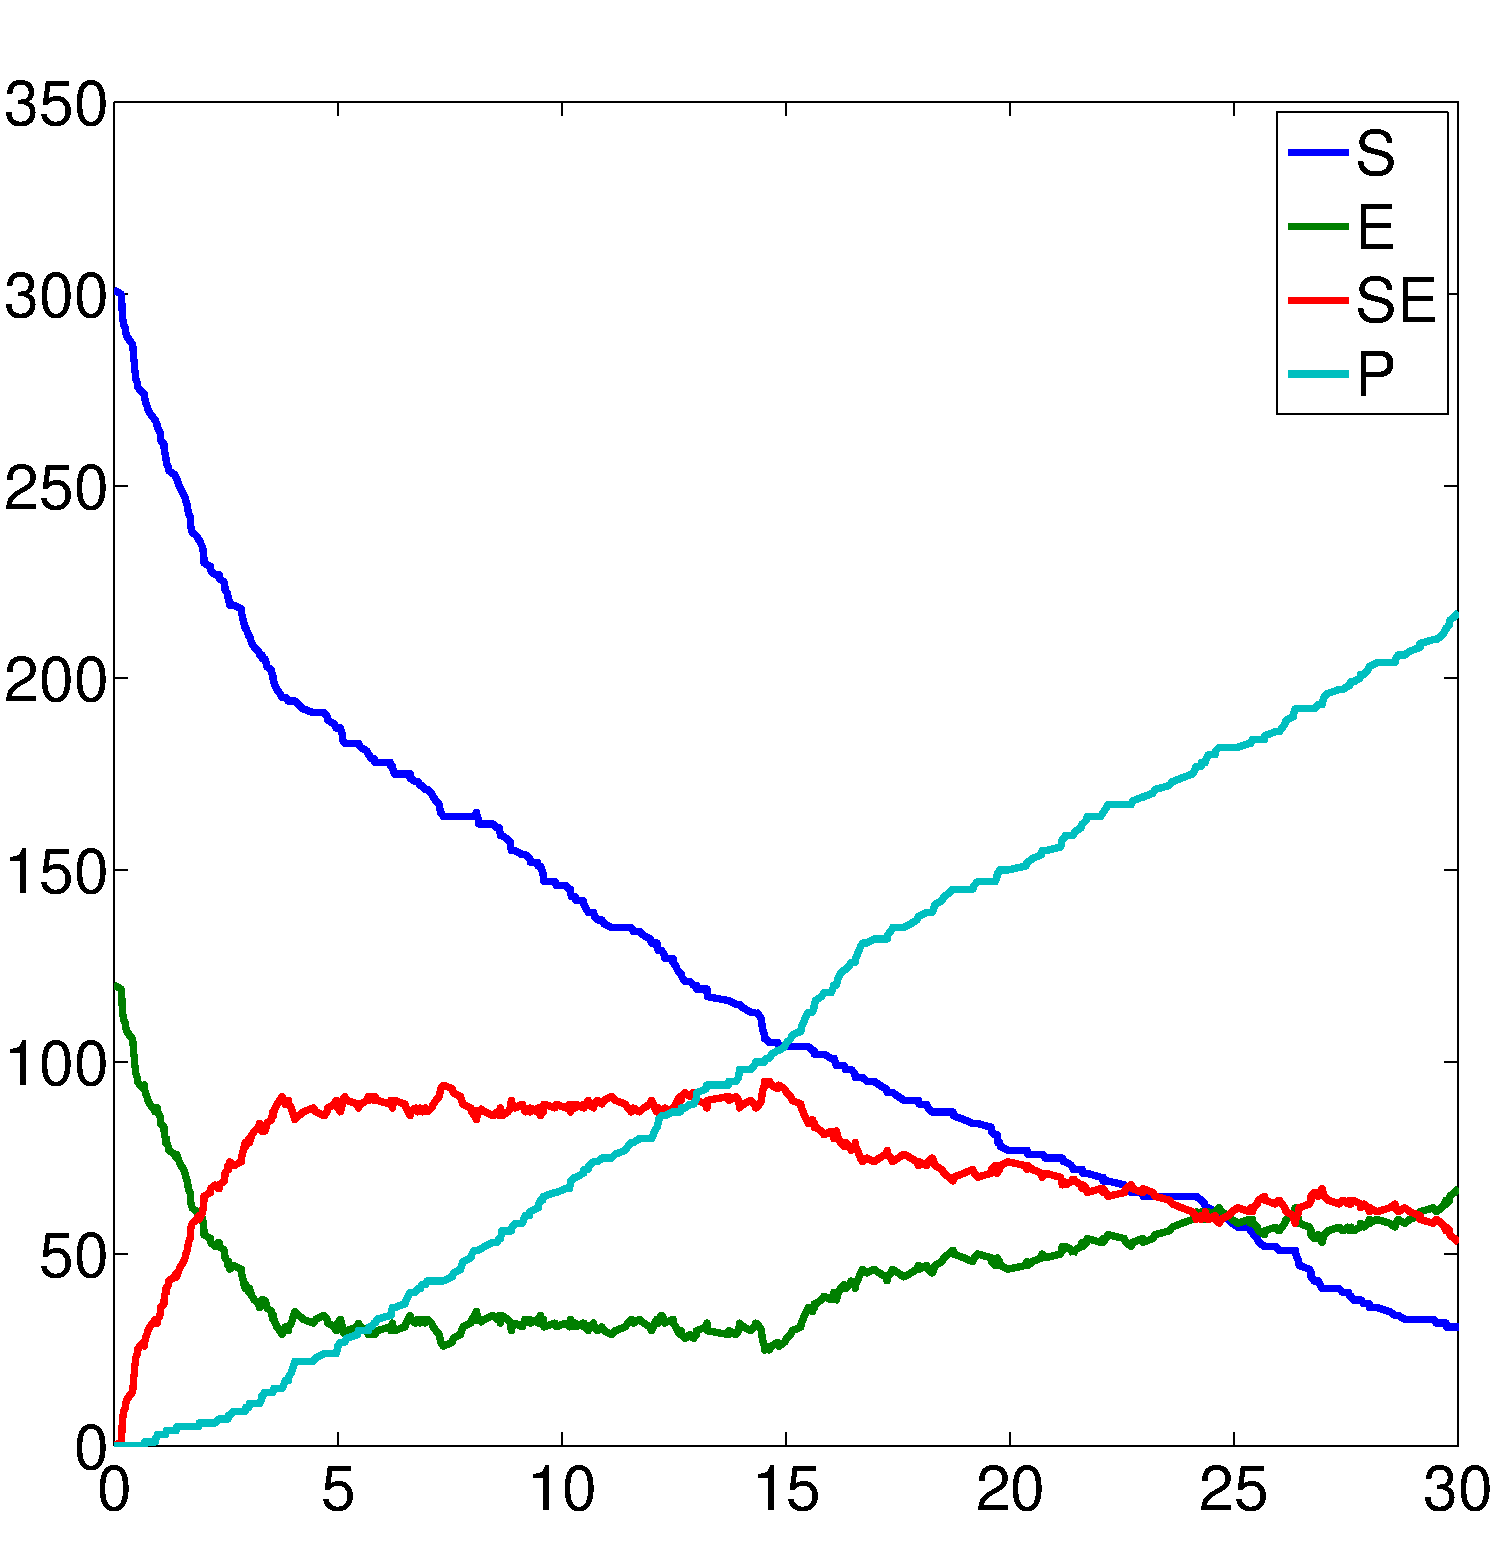
\includegraphics[width=0.5\textwidth]{figures/MM_ssa.pdf}
			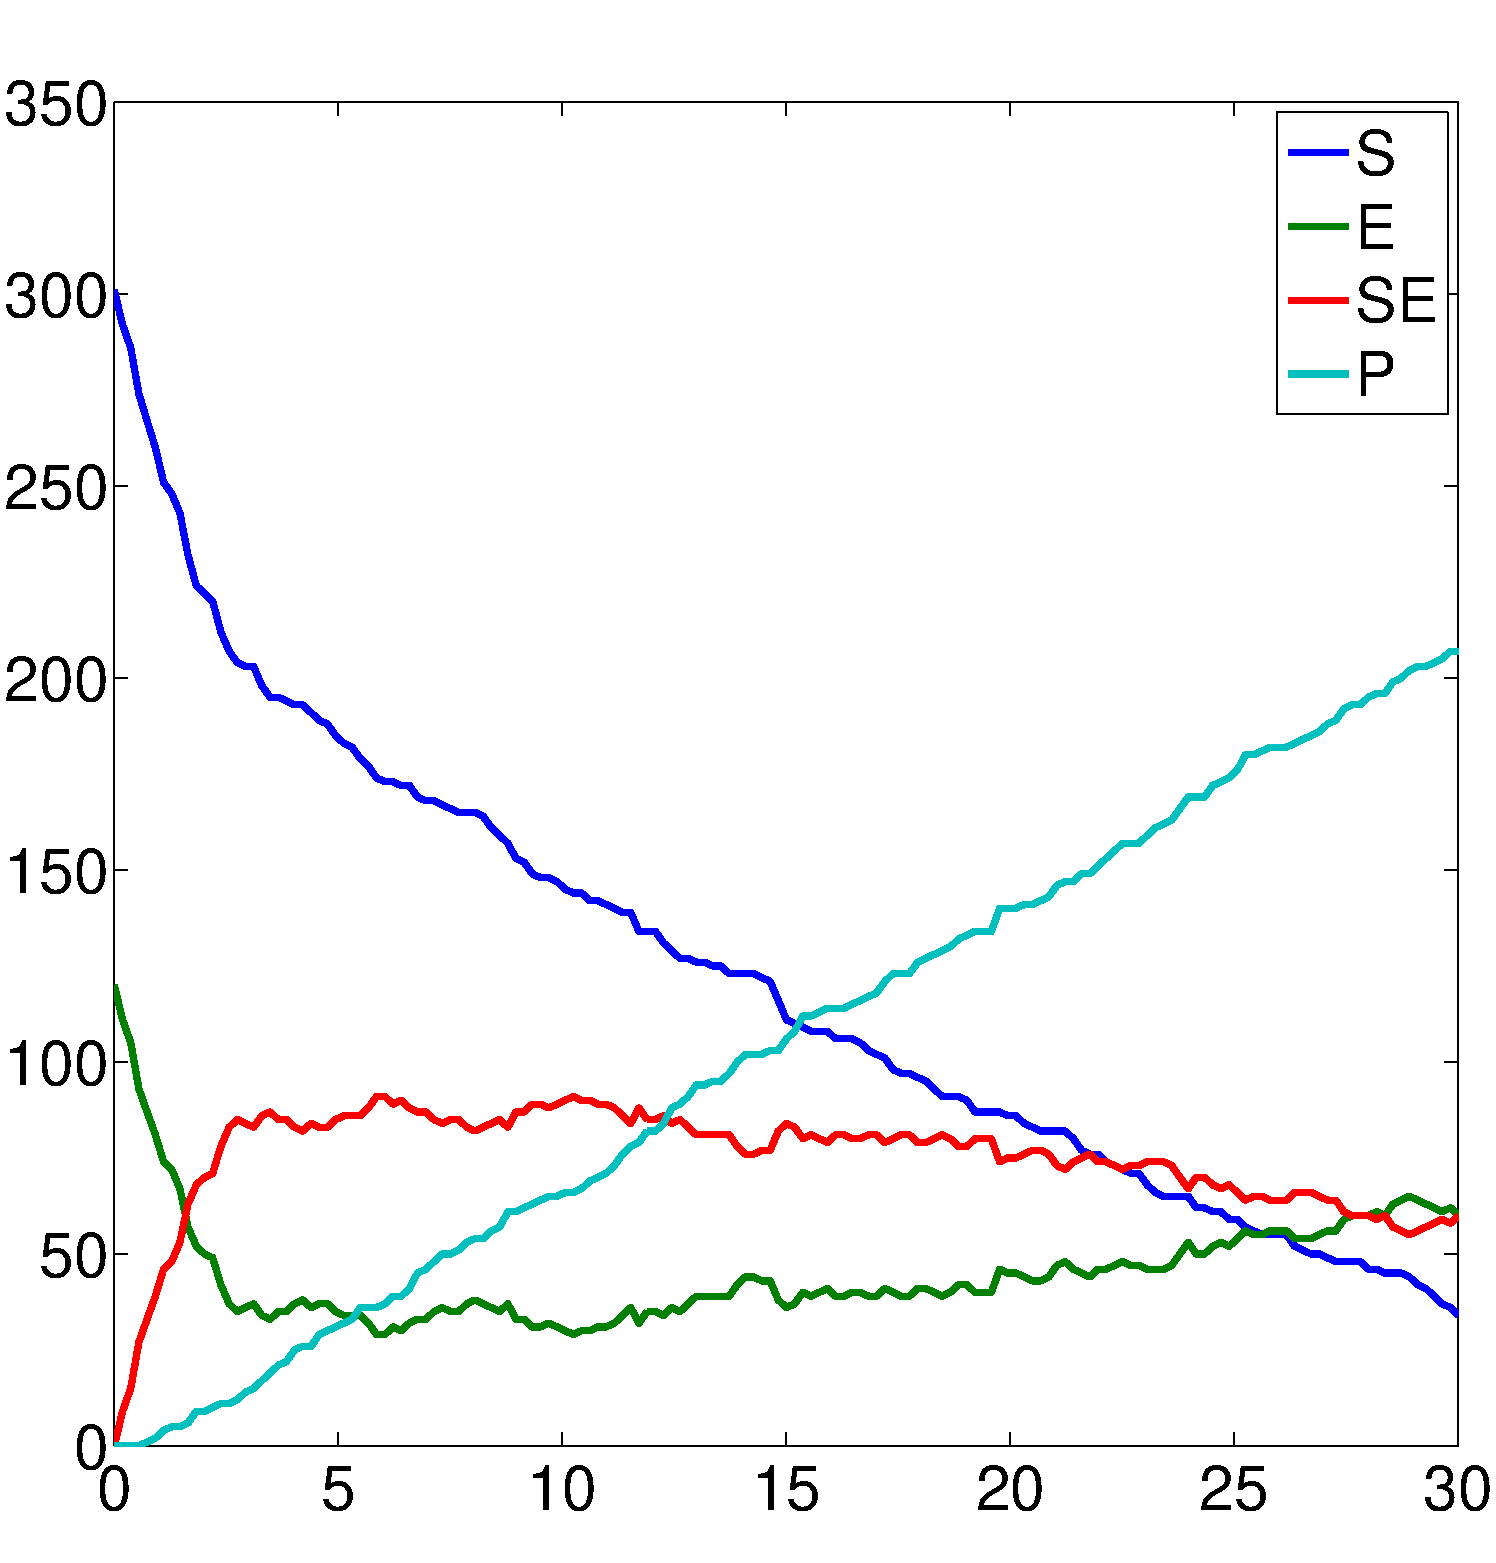
\includegraphics[width=0.5\textwidth]{figures/MM_tau.pdf}
			}
		\centerline{
			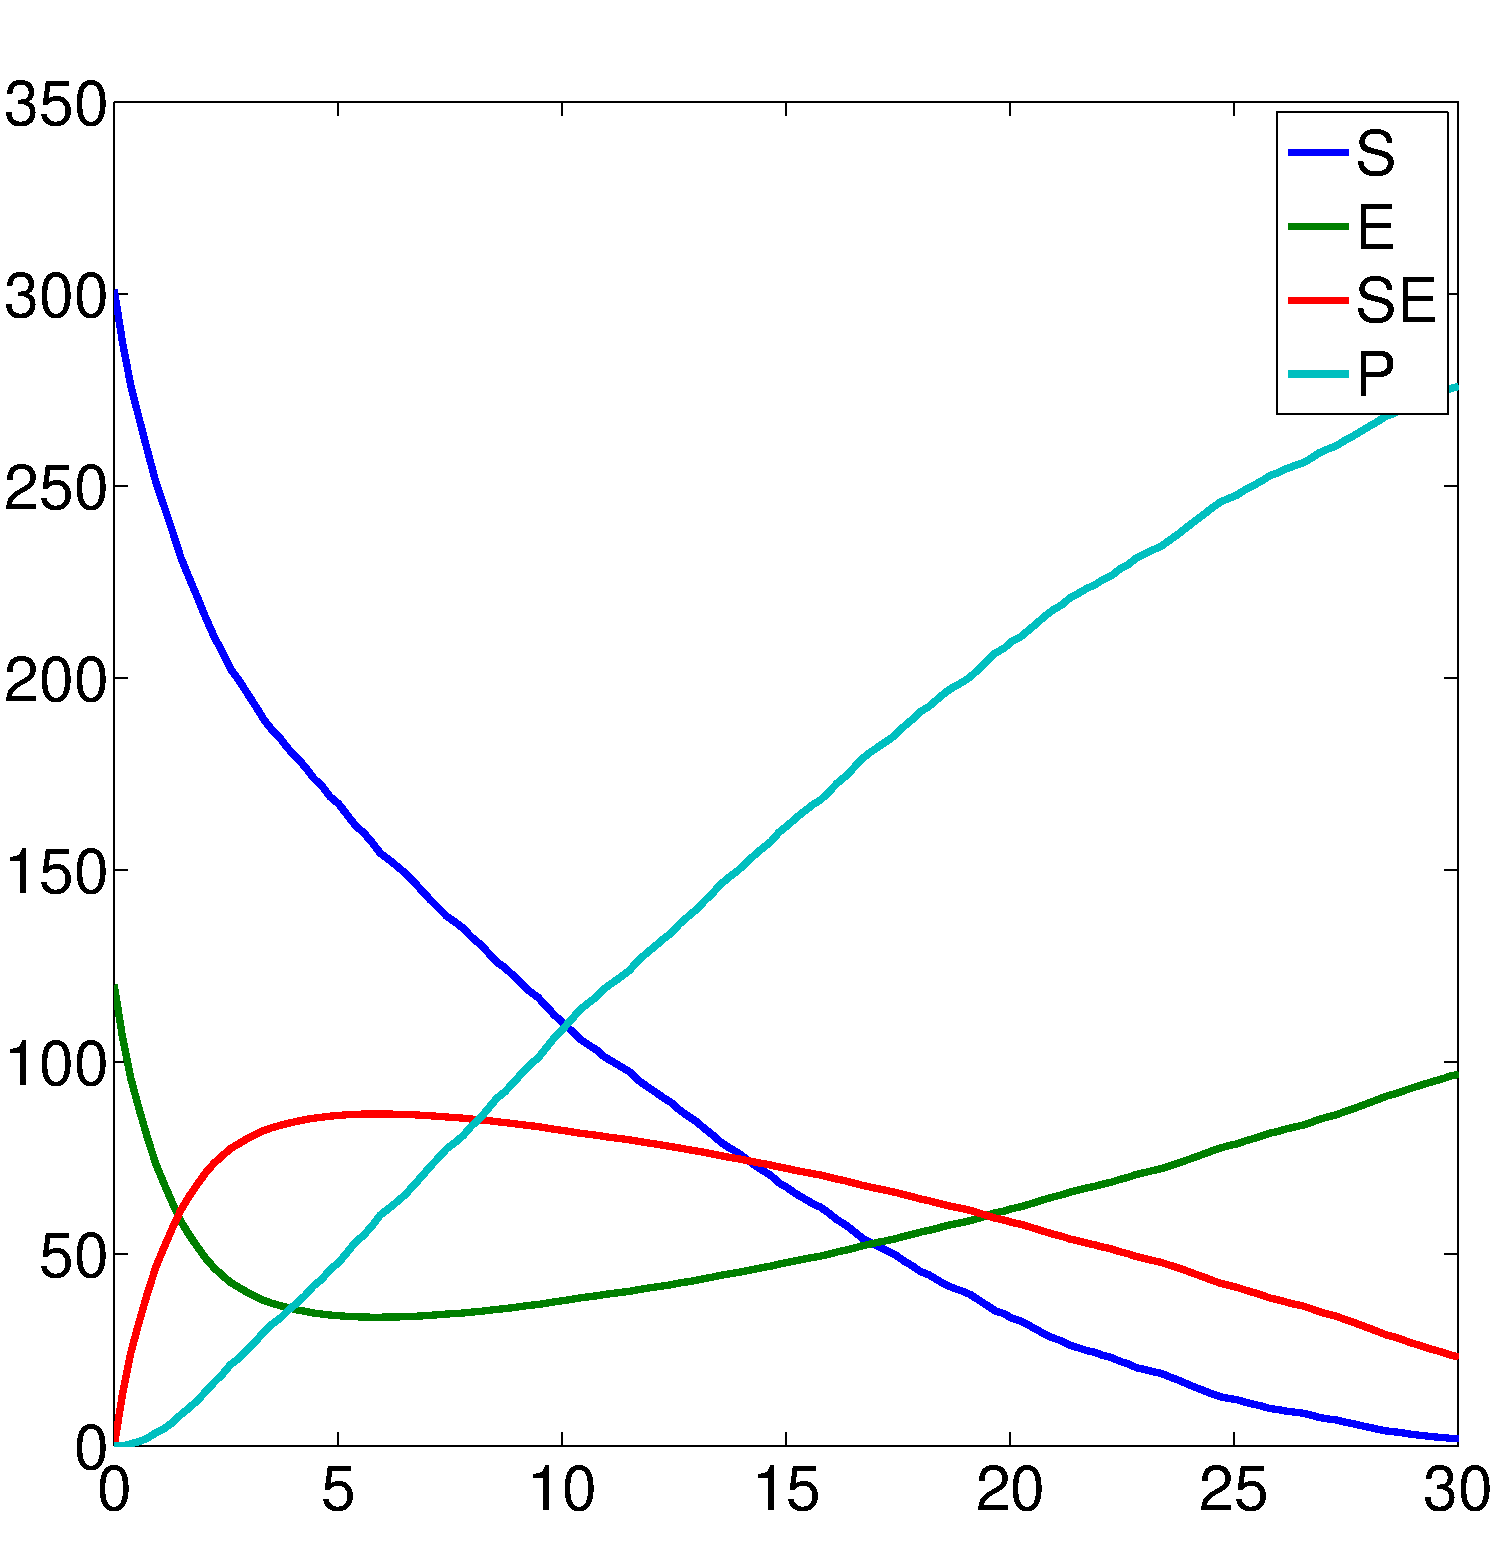
\includegraphics[width=0.5\textwidth]{figures/MM_cle.pdf}
			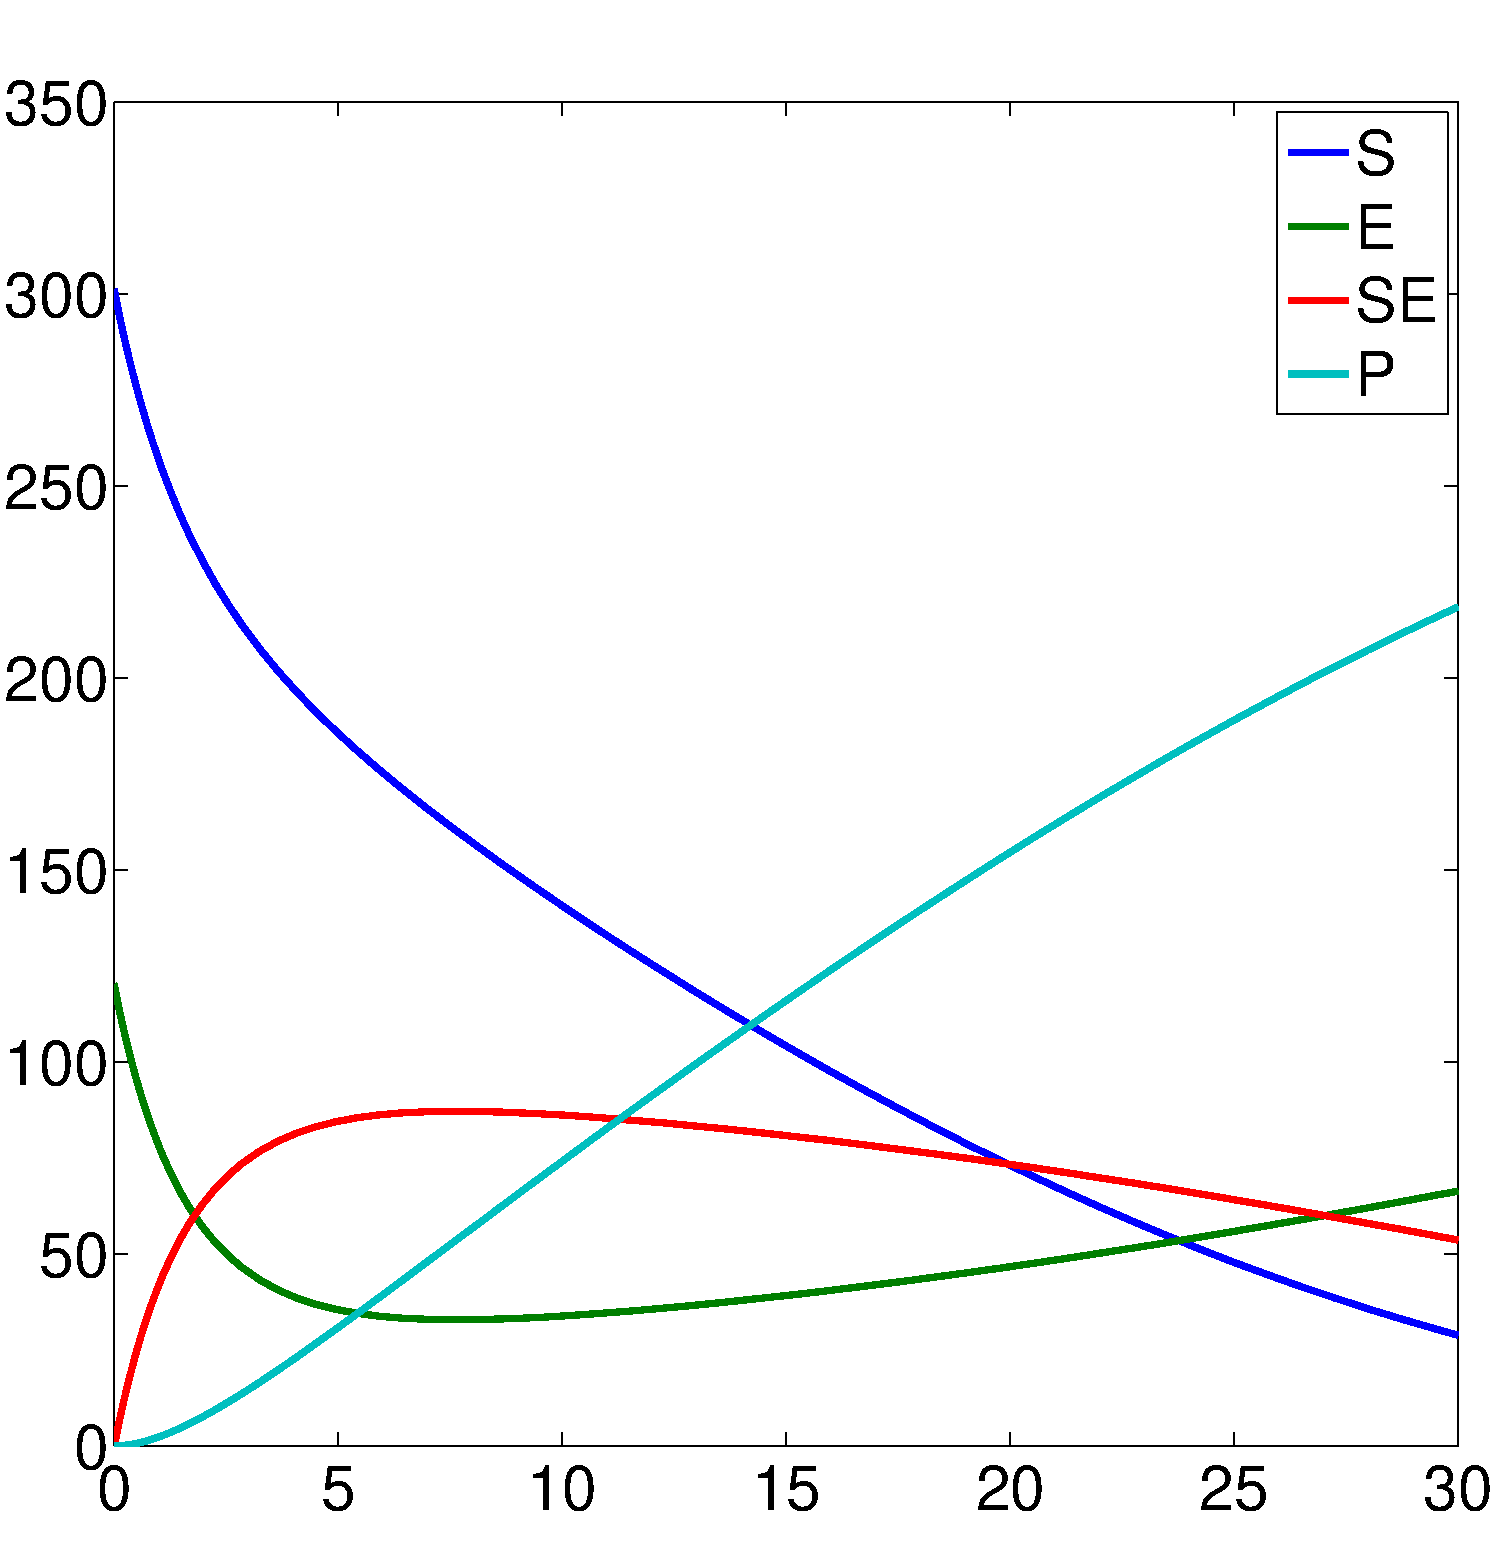
\includegraphics[width=0.5\textwidth]{figures/MM_rre.pdf}
			}
		\captionsetup{width=0.8\textwidth}
		\caption[Integration of the Michaelis Menten model over {$[0,30]$}]{Integration of the Michaelis Menten model over the interval $[0,30]$ using SSA (top left), tau-leaping (top right), LLA/CLE (bottom left), and RRE (bottom right). Vertical axis shows population amounts, horizontal axis shows simulation time. The value of $\tau$ employed by tau-leaping and LLA/CLE was automatically determined by MARS.}
		\label{mm_figure}
		\end{figure}

		\noindent
		Using the same initial population values of $(301,120,0,0)^T$, histograms of the end population were then produced by generating results from 10,000 trajectories. The same methods were applied, with the exception of GPU generation of trajectories being substituted for RRE, which would be ineligible for this test as it gives a deterministic prediction.\\
		\\
		The results are in the following Figure \ref{mm_hist_figure}.

		\begin{figure}[H]
		\centerline{
			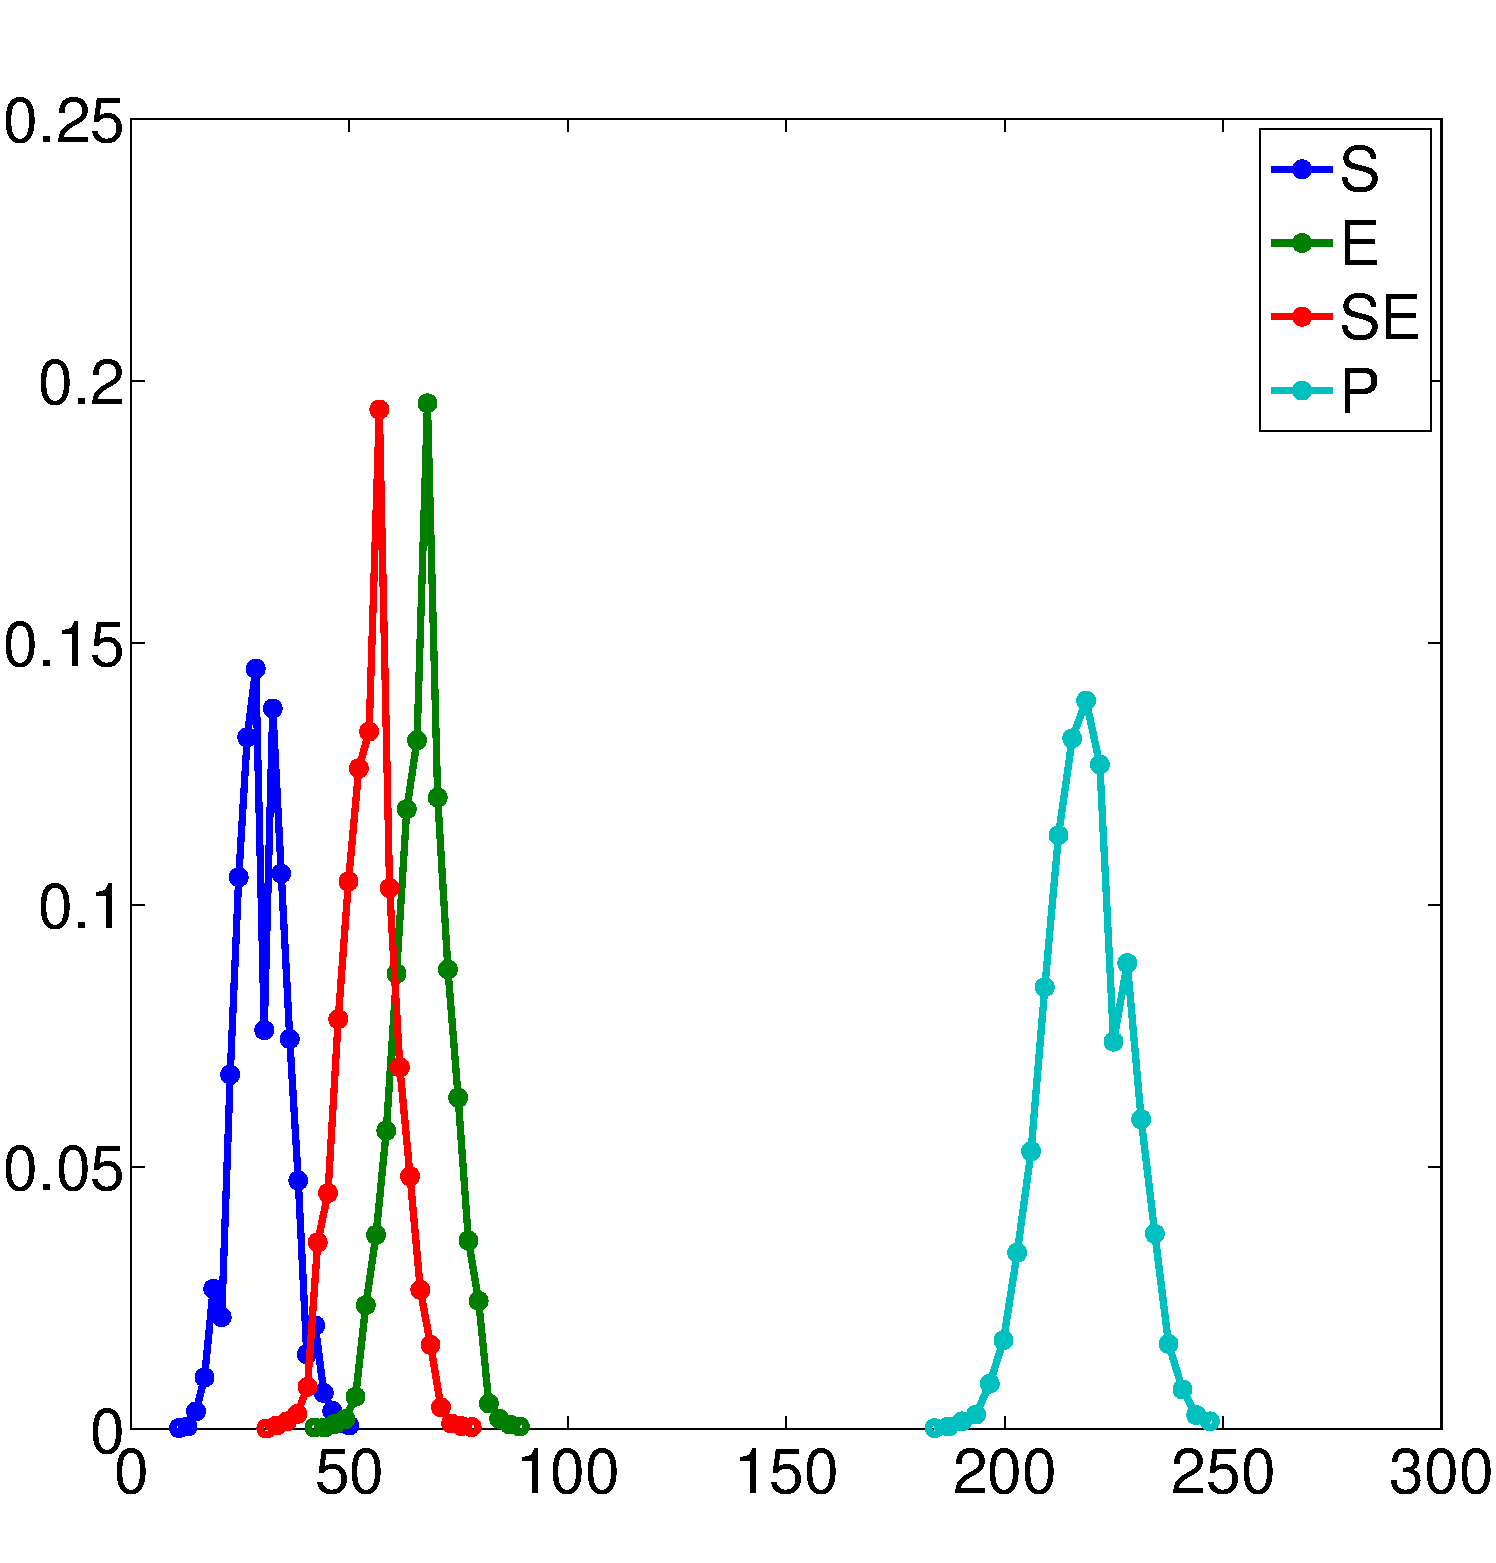
\includegraphics[width=0.5\textwidth]{figures/MM_ssa_hist.pdf}
			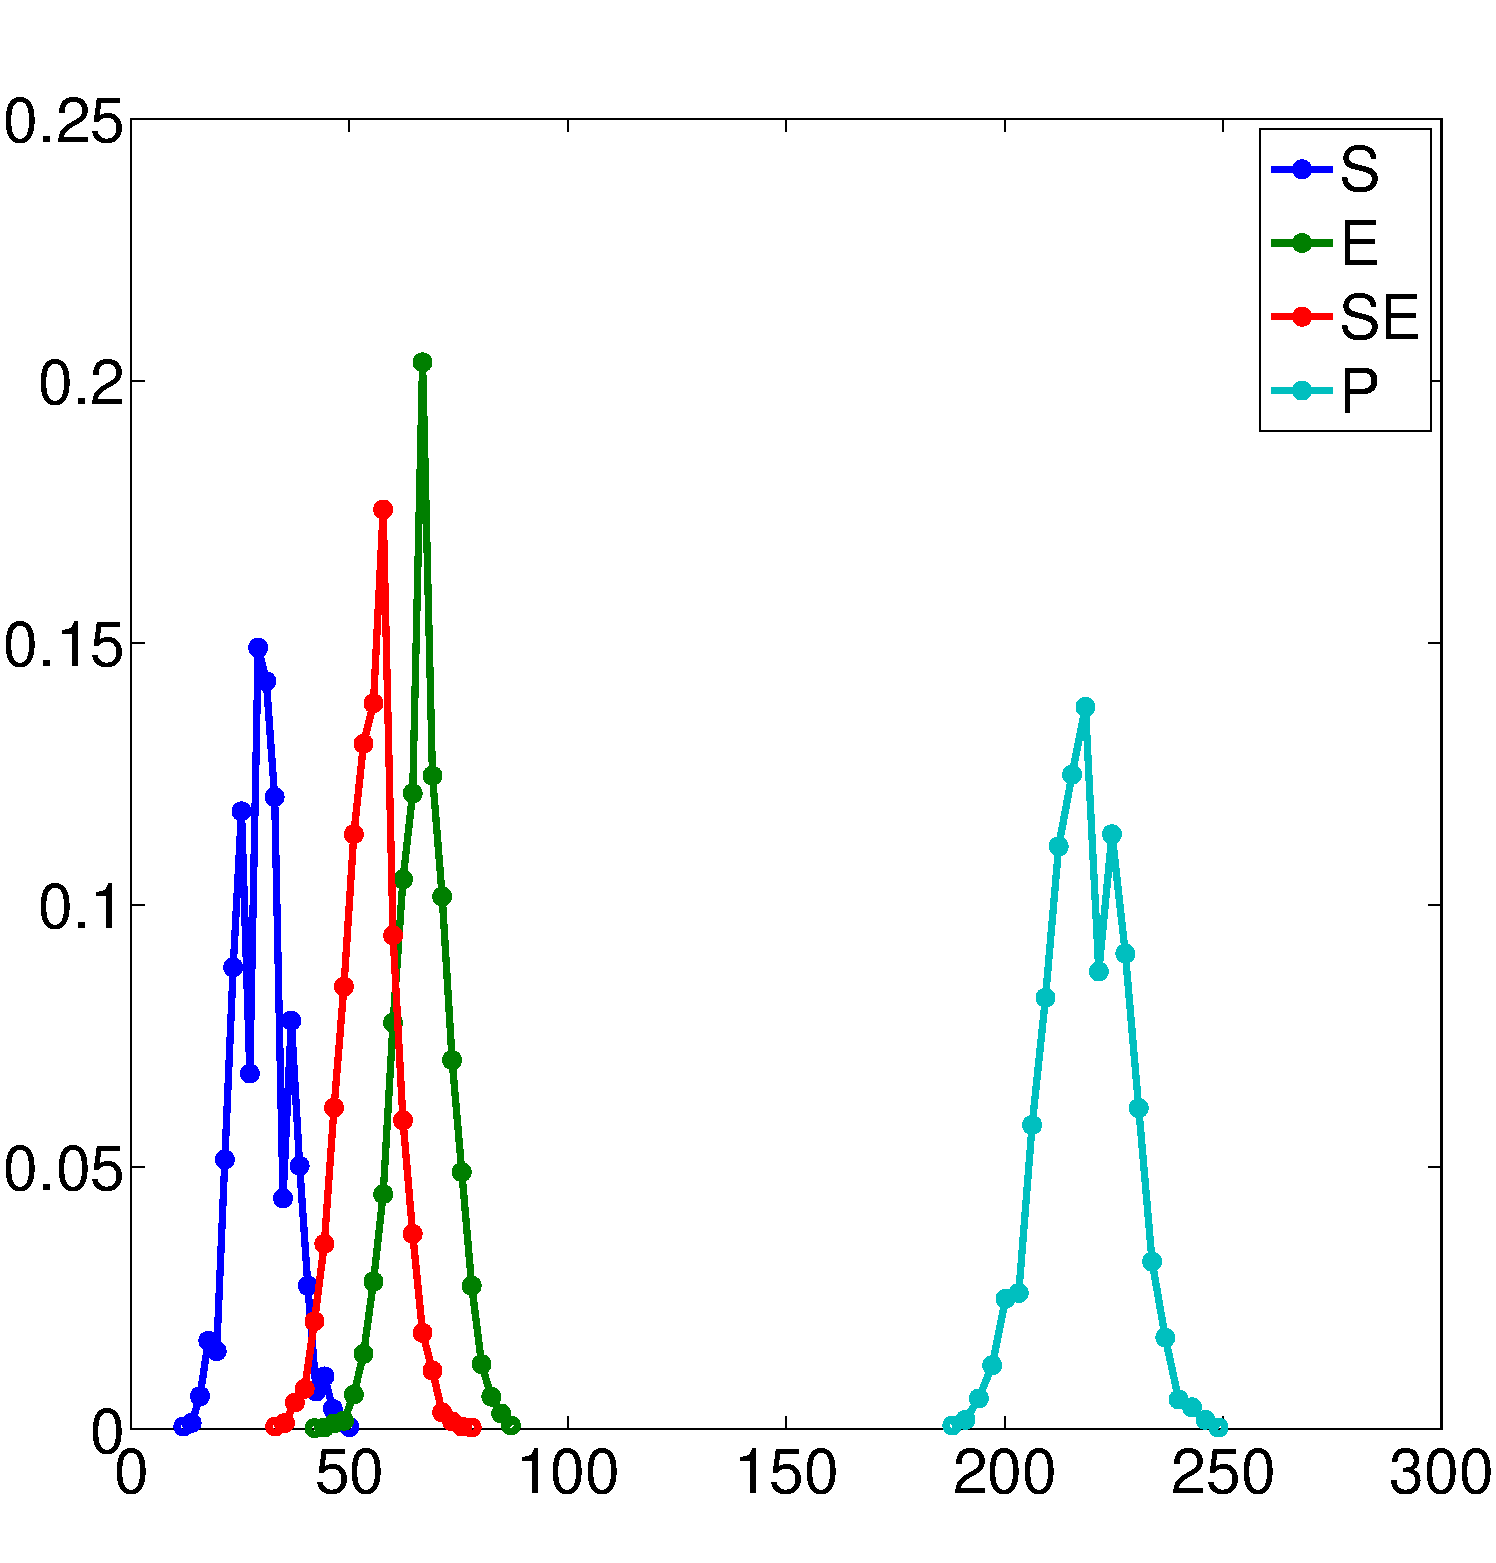
\includegraphics[width=0.5\textwidth]{figures/MM_tau_hist.pdf}
			}
		\centerline{
			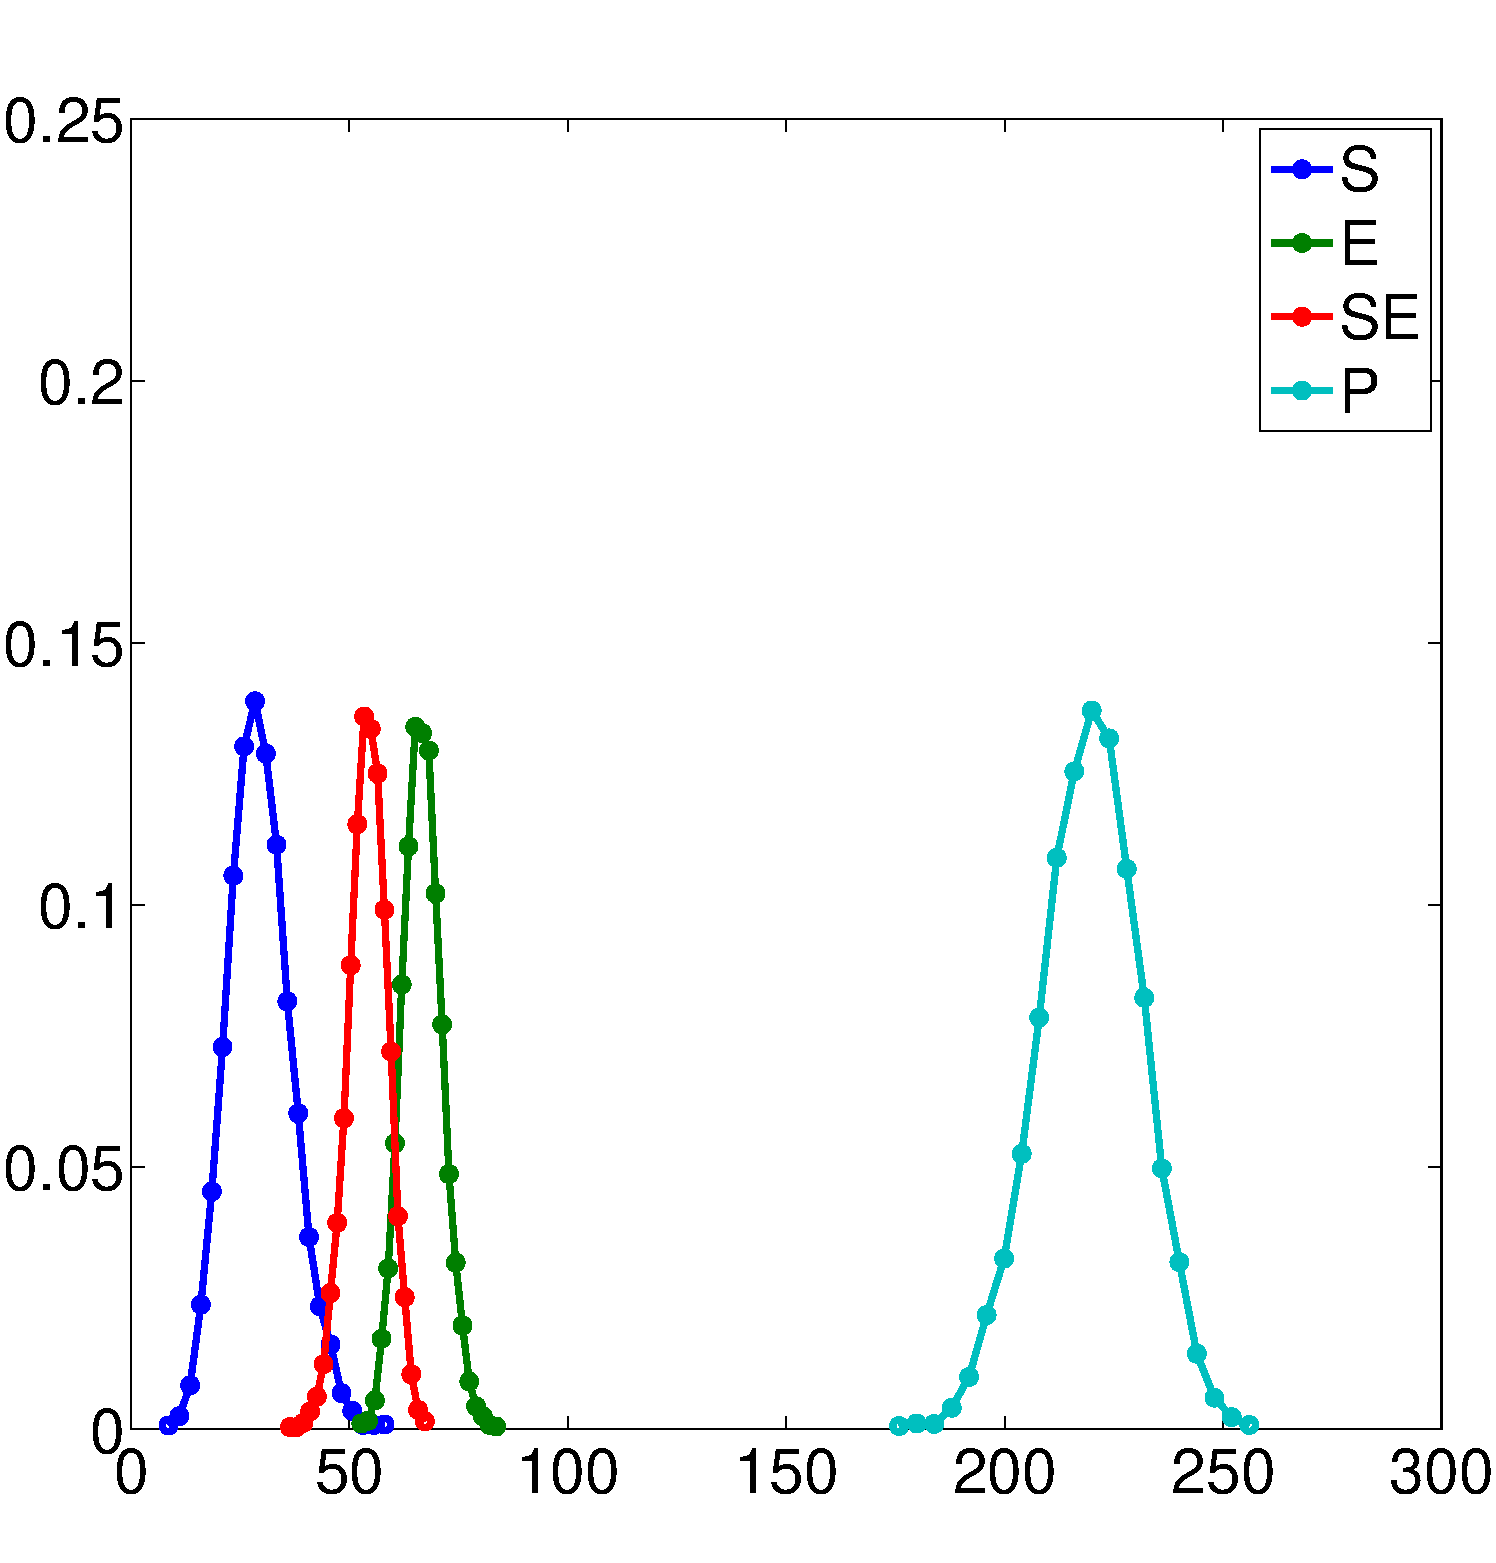
\includegraphics[width=0.5\textwidth]{figures/MM_cle_hist.pdf}
			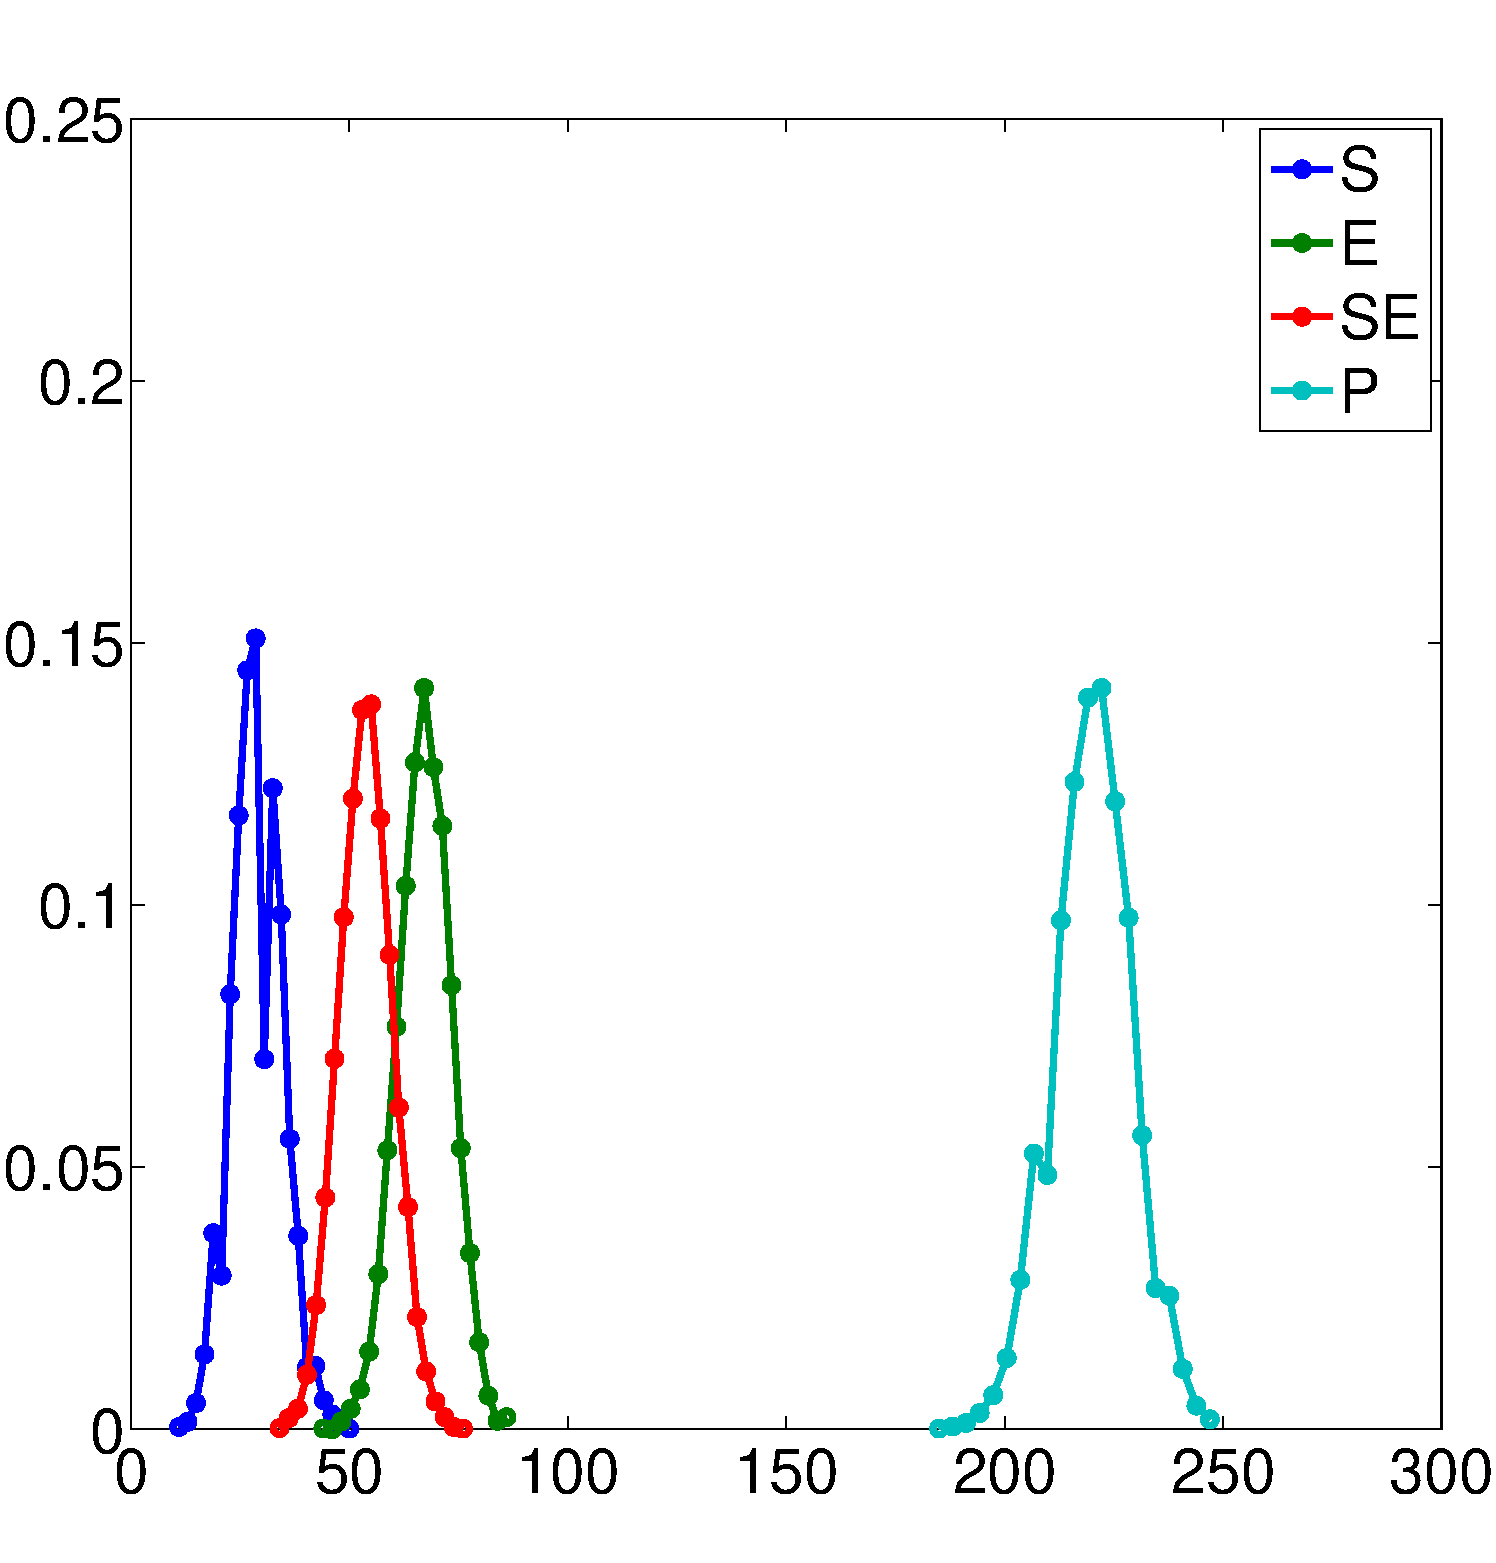
\includegraphics[width=0.5\textwidth]{figures/MM_gpu_hist.pdf}
			}
		\captionsetup{width=0.8\textwidth}
		\caption[Histogram of end populations of the Michaelis Menten model from 10,000 trajectories]{Histogram of population amounts computed on 10,000 trajectories, at the final time $T=30$, after simulation of the Michaelis Menten model over $[0,30]$ using SSA (top left), tau-leaping (top right), LLA/CLE (bottom left), and GPU (bottom right). The vertical axis shows frequency, the horizontal axis shows final population amounts. The value of $\tau$ utilized by tau-leaping and LLA/CLE was automatically determined by MARS.}
		\label{mm_hist_figure}
		\end{figure}

	\section{Schl\"{o}gl Model}

		The Schl\"{o}gl model \cite{schlogl} consists of 3 species engaged in two reversible reactions (which are split into four reactions). This model contains a bifurcation based on the value of the initial population of one of the species. This will be discussed in the next section.\\
		\\
		The relevant model data presented in Table \ref{mm_table}.

		\begin{table}[H]
		\[
		\begin{array}{l@{\hspace*{10mm}}r@{\ }c@{\ }l@{\hspace*{10mm}}l@{\hspace*{10mm}}l}
		\multicolumn{4}{c}{\text{{\huge\phantom{$I_{I_I}$}}Reactions}} & \multicolumn{1}{c}{\text{Propensities}} & \multicolumn{1}{c}{\text{Reaction rates}}\\
		\hline
		R_1 	& A+2X & \stackrel{c_1}{\rightarrow} & 3X 	& a_1(\mathbf{x})=c_1AX(X-1)/2 	 & c_1 = 3 \times 10^{-3}
		\\\\
		R_2 	& 3X & \stackrel{c_2}{\rightarrow} & A + 2X  	& a_2(\mathbf{x})=c_2X(X-1)(X-2)/6		& c_2 = 10^{-4}
		\\\\
		R_3 	& B & \stackrel{c_3}{\rightarrow} & X 		& a_3(\mathbf{x}) = c_3 B 					& c_3 = 10^{-3}
		\\\\
		R_4 	& X & \stackrel{c_4}{\rightarrow} & B 		& a_3(\mathbf{x}) = c_4 X 					& c_4 = 3.5
		\end{array}
		\]
		\captionsetup{width=0.8\textwidth}
		\caption{Schl\"{o}gl model}
		\label{schlogl_table}
		\end{table}

		\noindent
		Additionally, the populations of species $A$ and $B$ are held constant, making $X$ the only species of interest. The model is integrated with initial population values for $(A,B,X)^T$ of $(10^5,2 \times 10^5,248)^T$. Single trajectories were generated over the interval $[0,15]$ employing SSA, tau-leaping, LLA/CLE, and RRE methods of the MARS software.\\
		\\
		Numerical results for the Schl\"{o}gl model are shown in Figure \ref{schlogl_figure}.

		\begin{figure}[H]
		\centerline{
			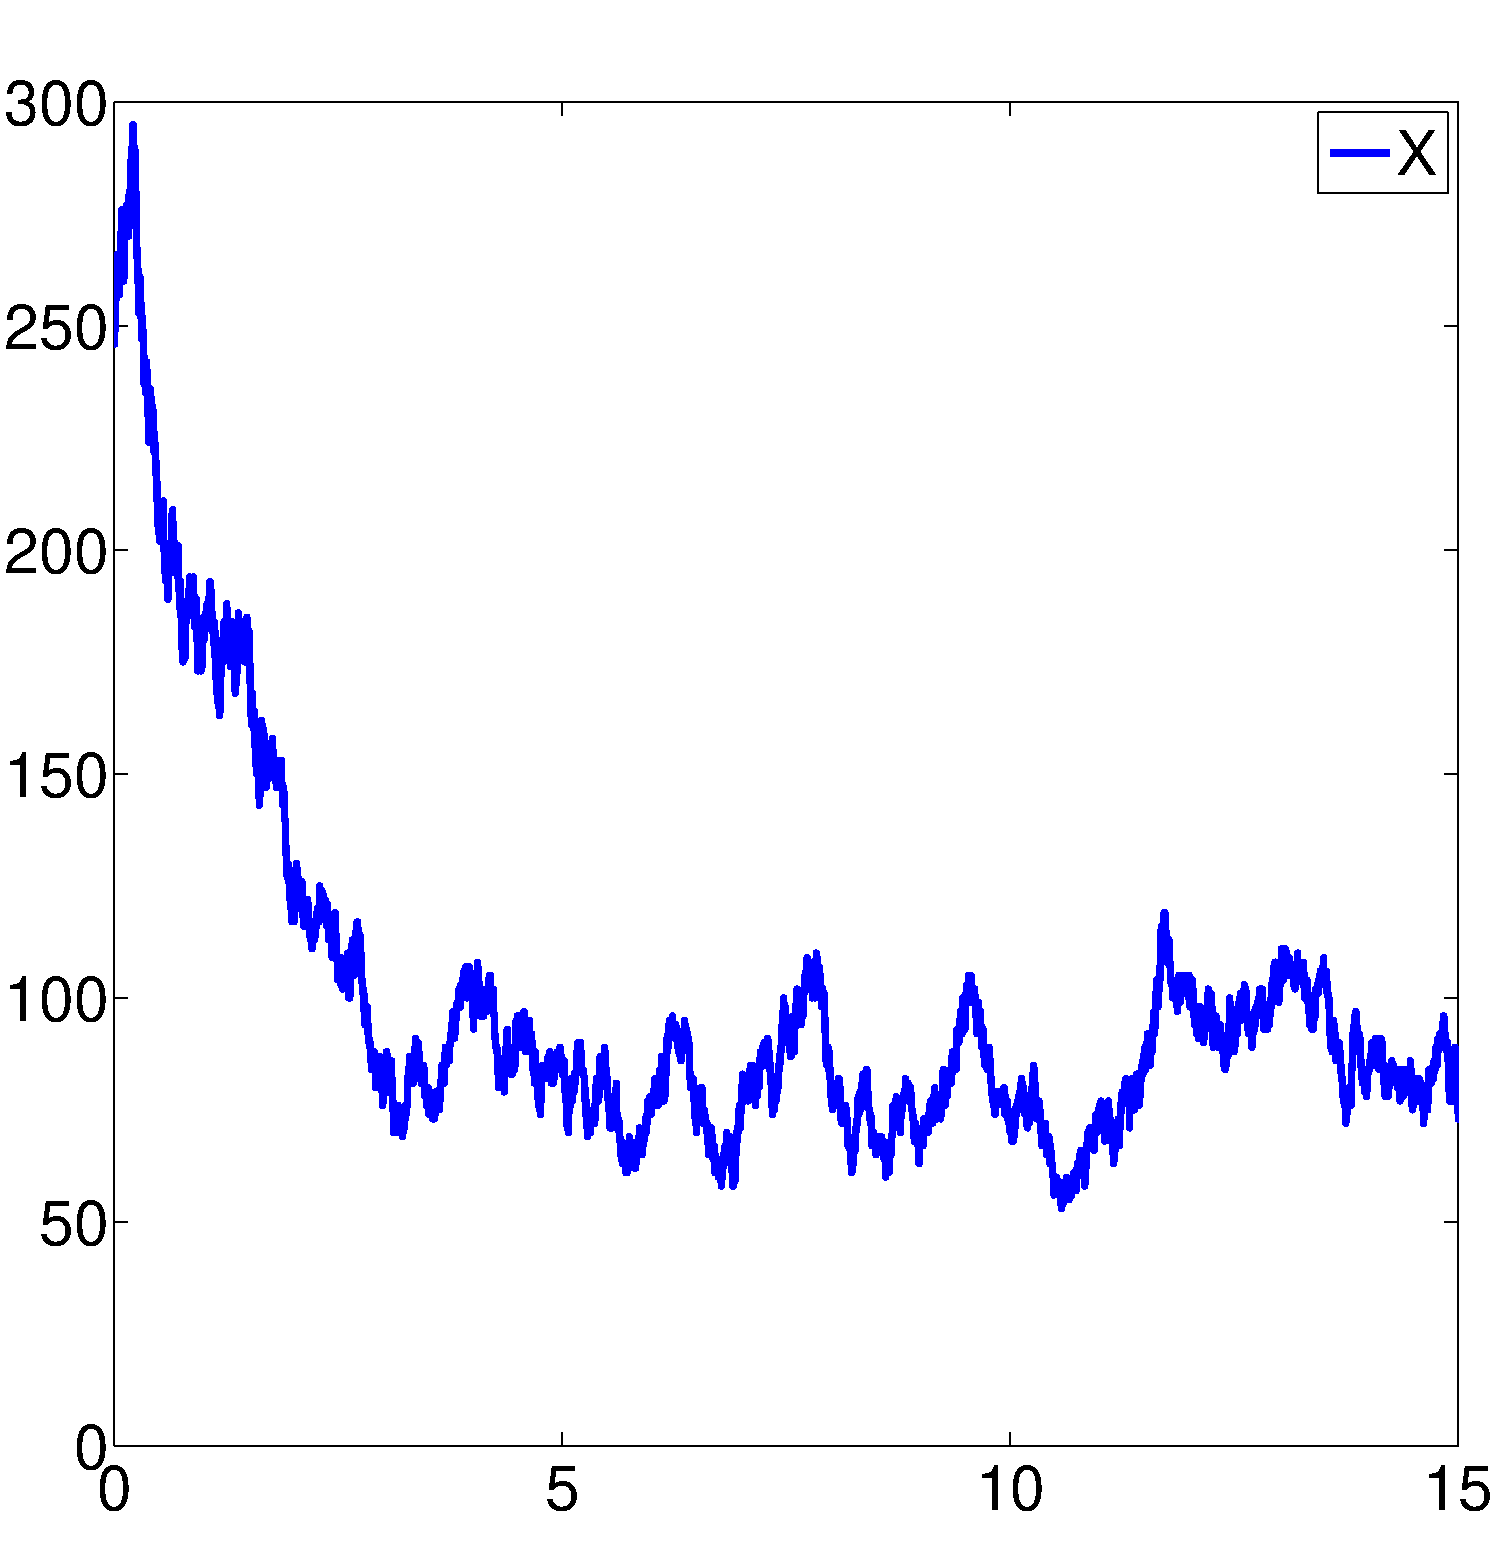
\includegraphics[width=0.5\textwidth]{figures/Schlogl_ssa.pdf}
			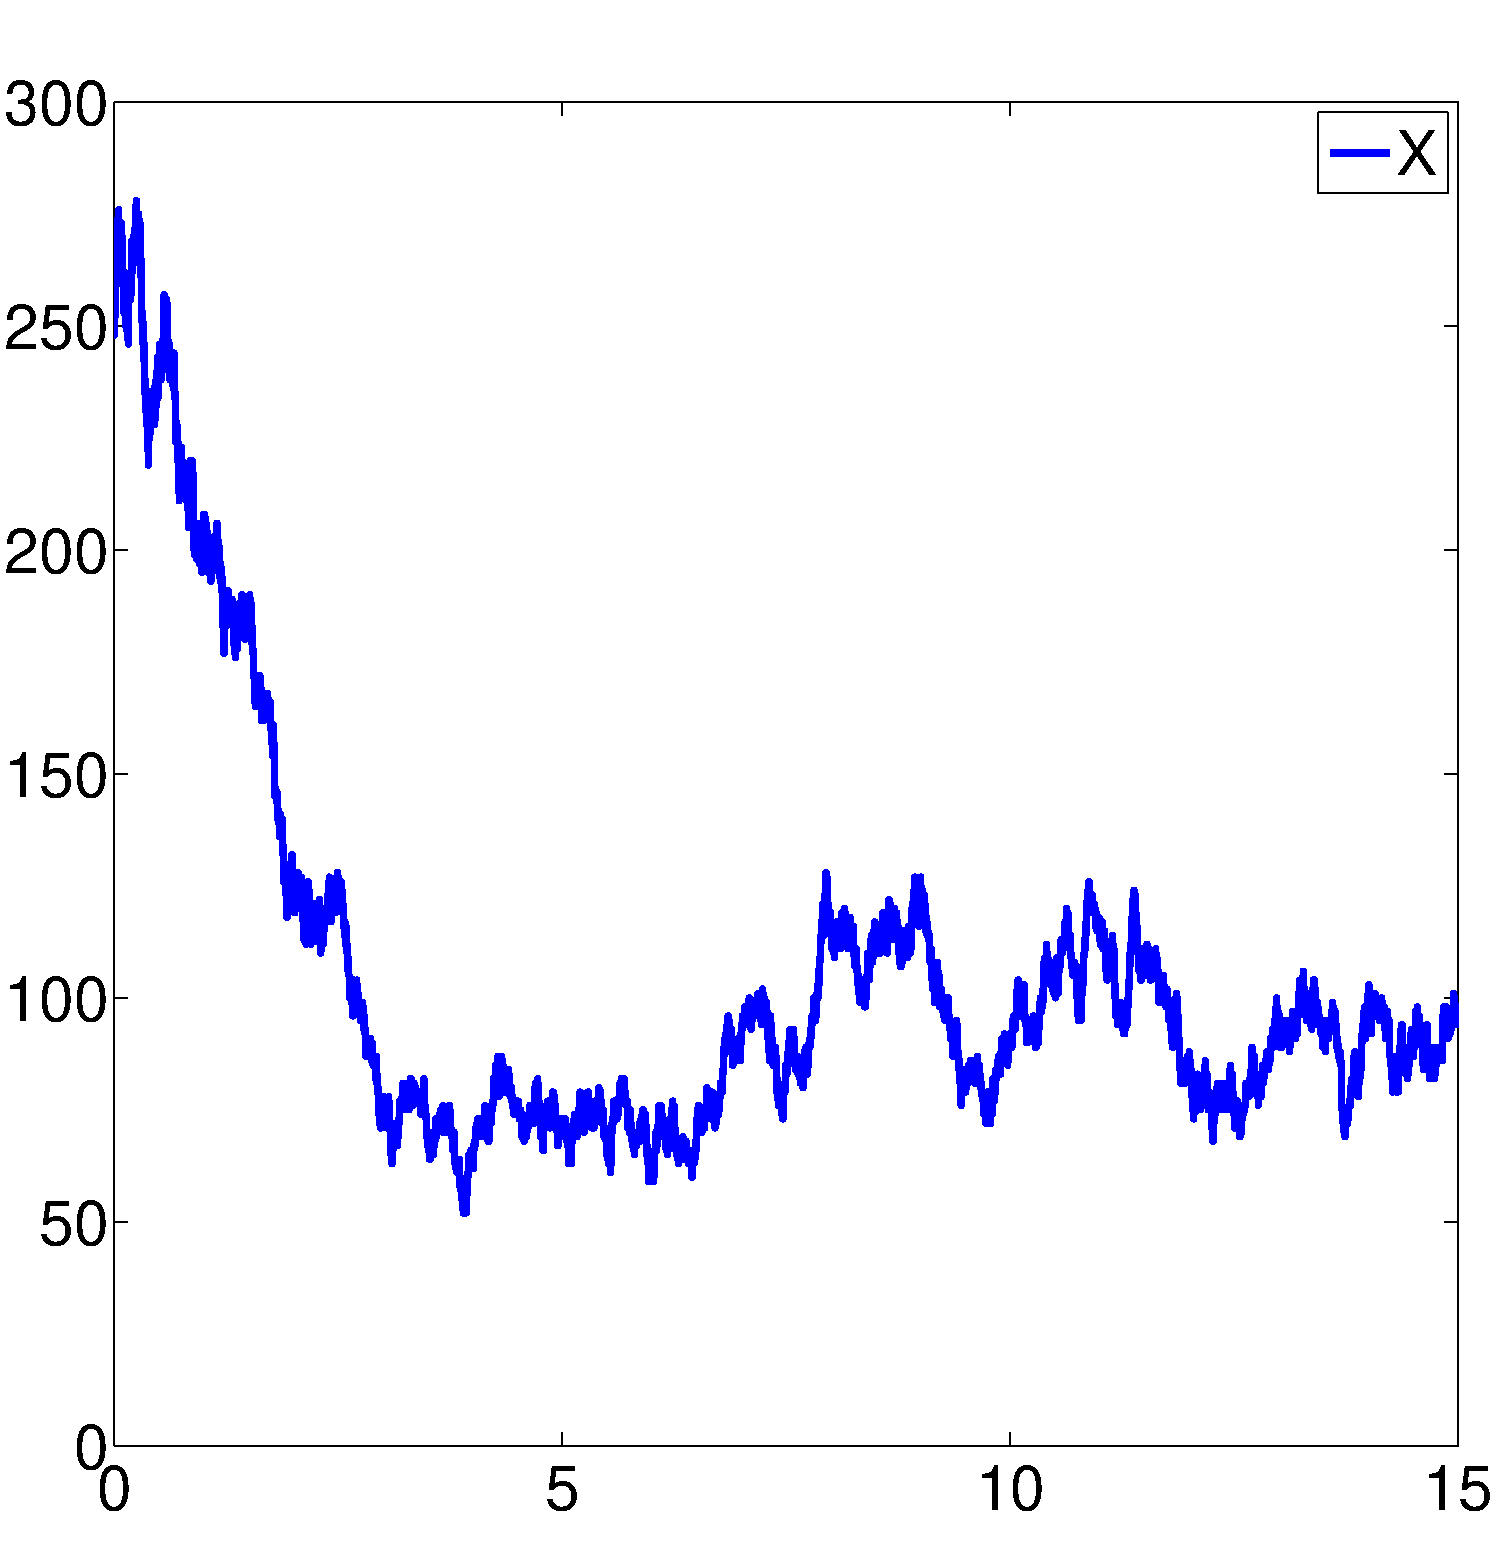
\includegraphics[width=0.5\textwidth]{figures/Schlogl_tau.pdf}
			}
		\centerline{
			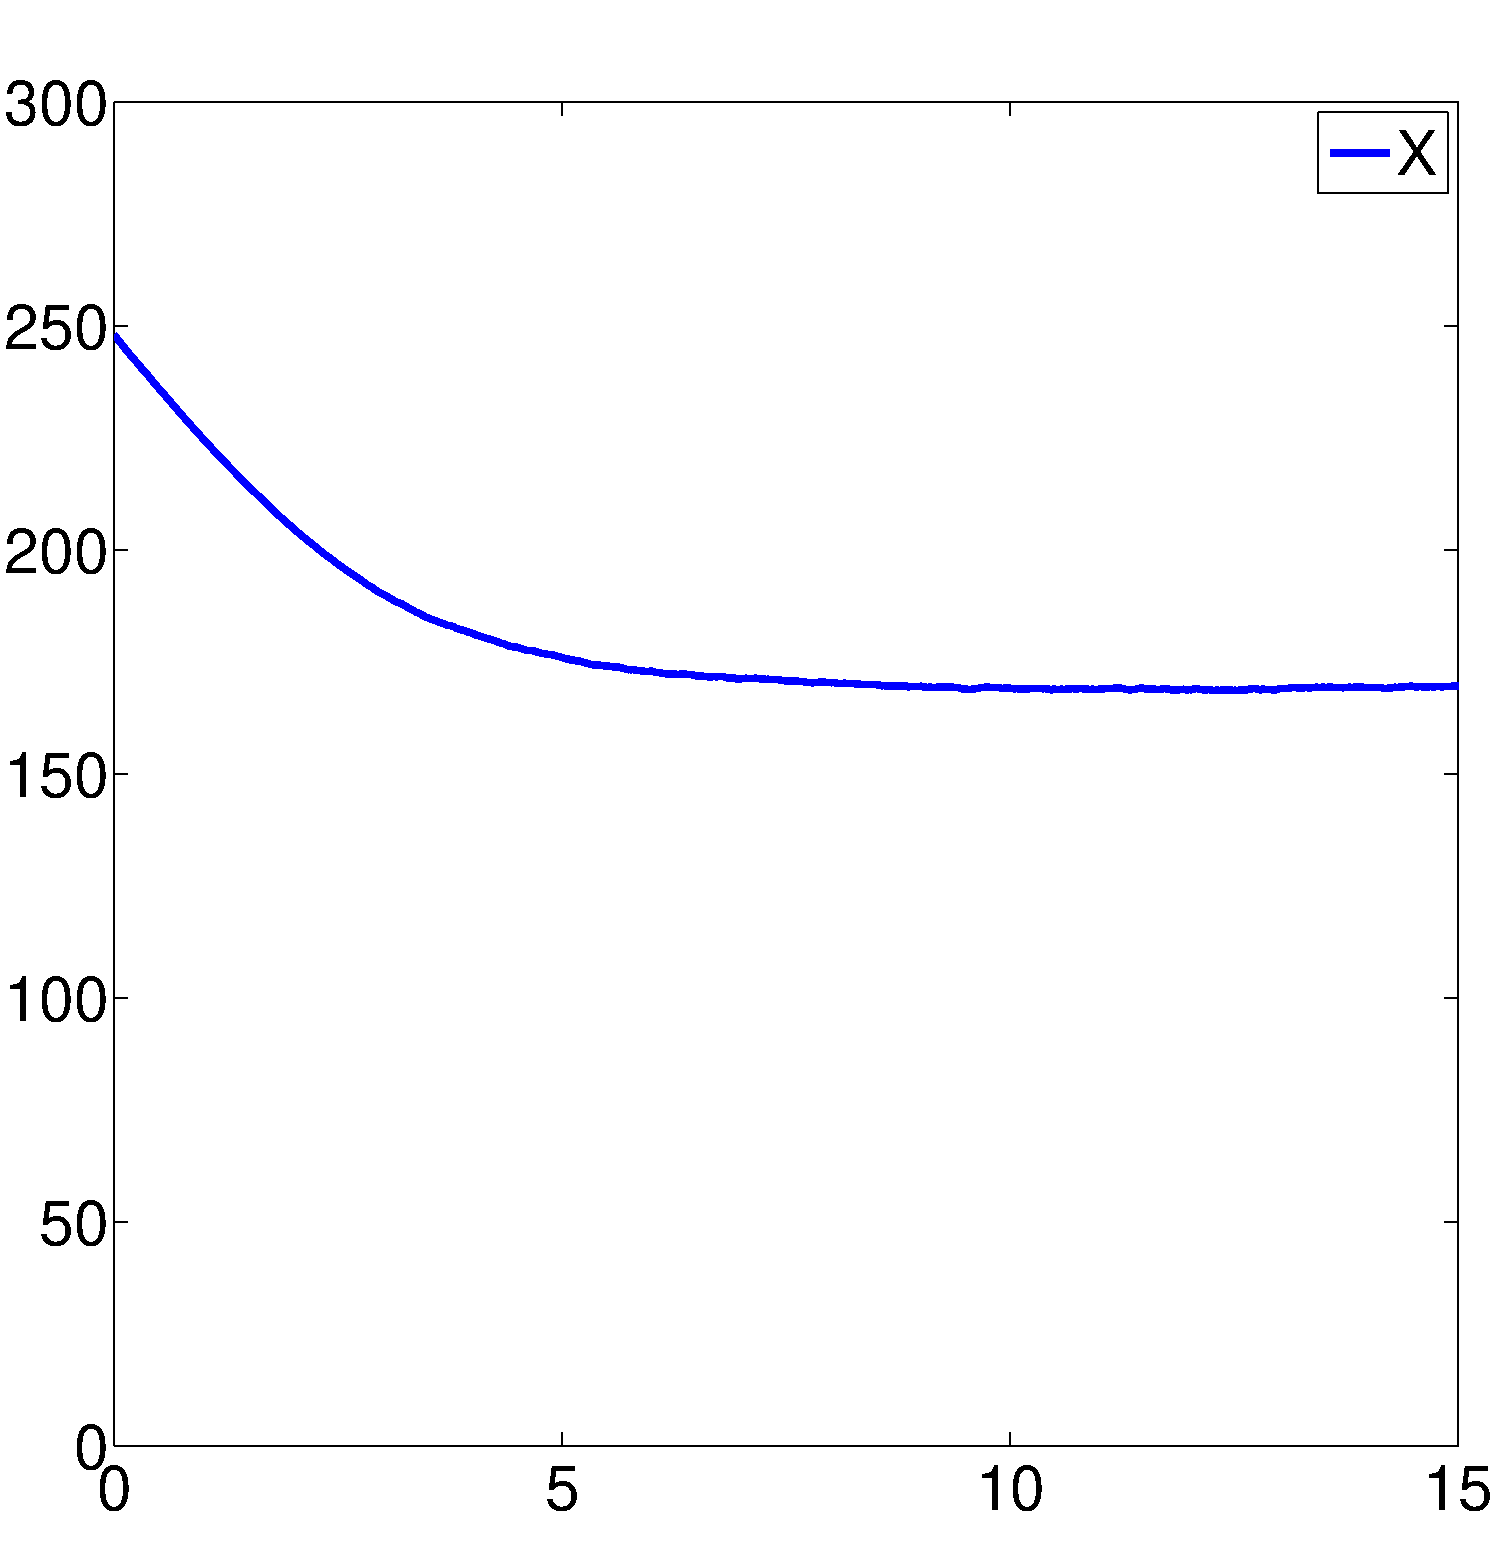
\includegraphics[width=0.5\textwidth]{figures/Schlogl_cle.pdf}
			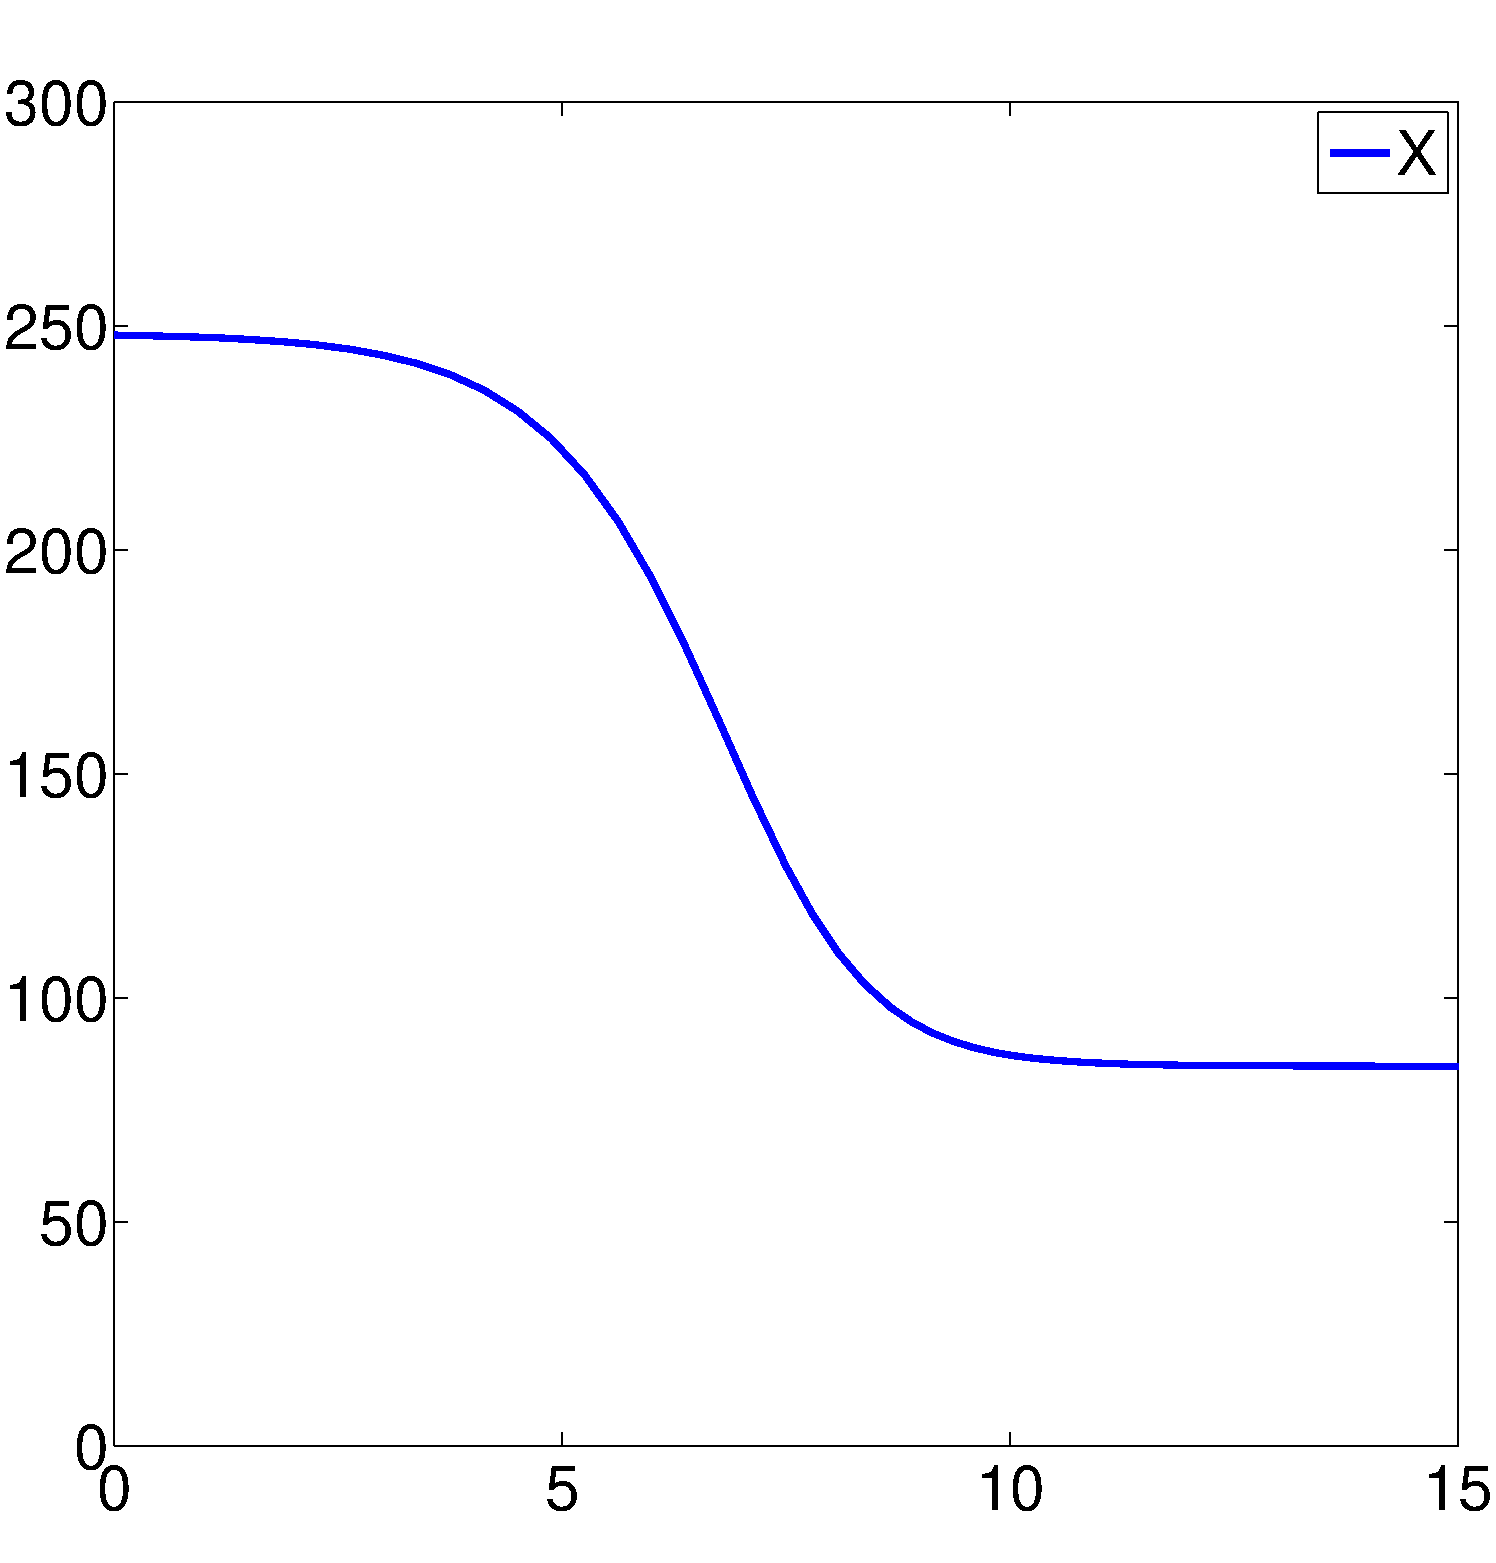
\includegraphics[width=0.5\textwidth]{figures/Schlogl_rre.pdf}
			}
		\captionsetup{width=0.8\textwidth}
		\caption[Integration of the Schl\"{o}gl model over {$[0,15]$}]{Integration of the Schl\"{o}gl model over the interval $[0,15]$ using SSA (top left), tau-leaping (top right), LLA/CLE (bottom left), and the default MARS solver for the RRE (bottom right). The vertical axis shows population amounts, while the horizontal axis shows simulation time. The value of $\tau$ utilized by tau-leaping and LLA/CLE was automatically determined by MARS.}
		\label{schlogl_figure}
		\end{figure}

		\noindent
		It is interesting to note that the LLA/CLE method exhibits almost deterministic behaviour, and the lack of noise makes the initial downward trajectory shallower, and so the estimate it produces is much higher than the noisier SSA and tau-leaping methods.\\
		\\
		With the same initial population values of $(10^5,2 \times 10^5,248)^T$, histograms of the populations at the final time were then produced by simulating 10,000 trajectories. The same methods were used, with the exception of GPU generation of trajectories being substituted for RRE solver, which would be ineligible for this test. Again, the RRE model was not included as it predicts the dynamics of the biochemical system deterministically.\\
		\\
		The results are in the following Figure \ref{schlogl_hist_figure}.

		\begin{figure}[H]
		\centerline{
			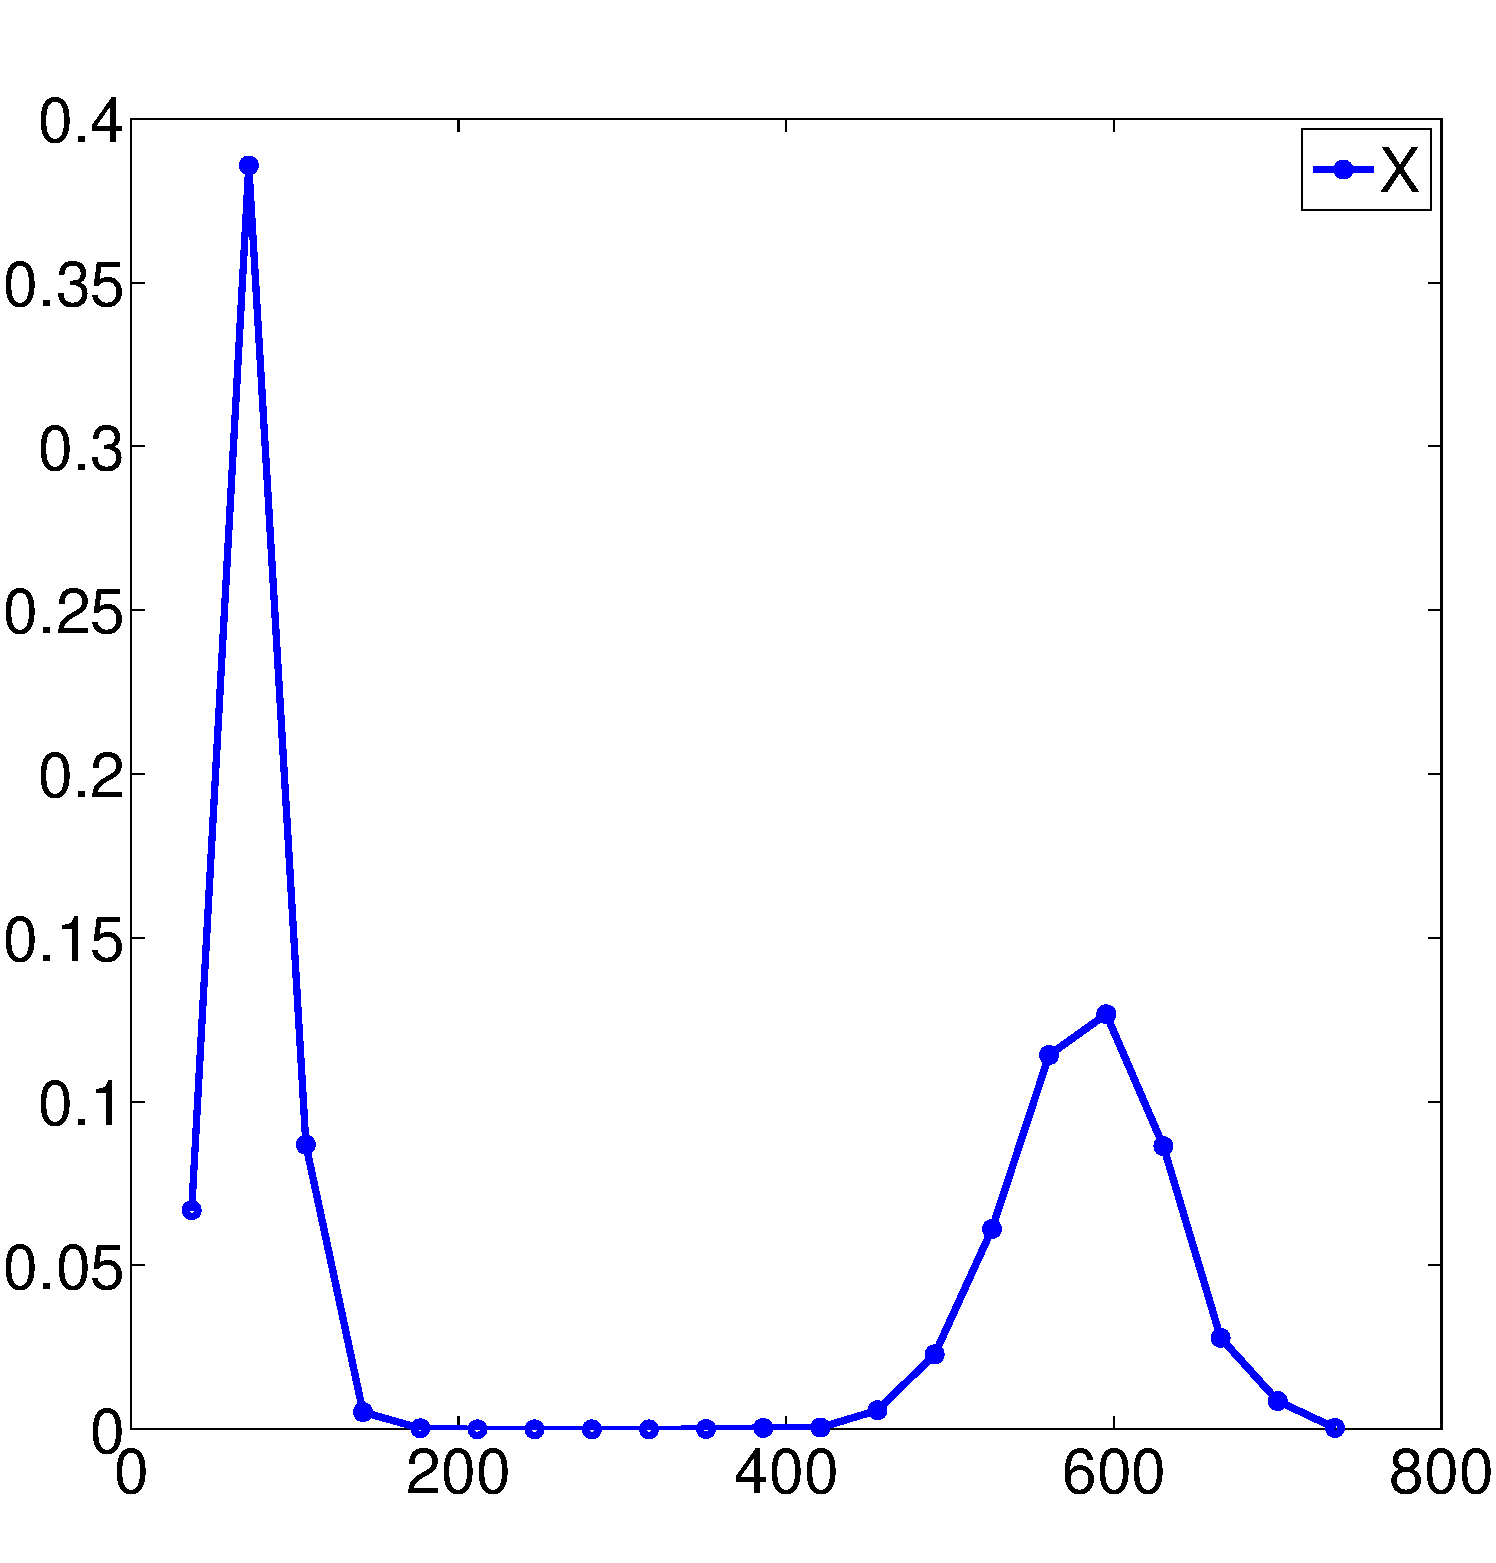
\includegraphics[width=0.5\textwidth]{figures/Schlogl_ssa_hist.pdf}
			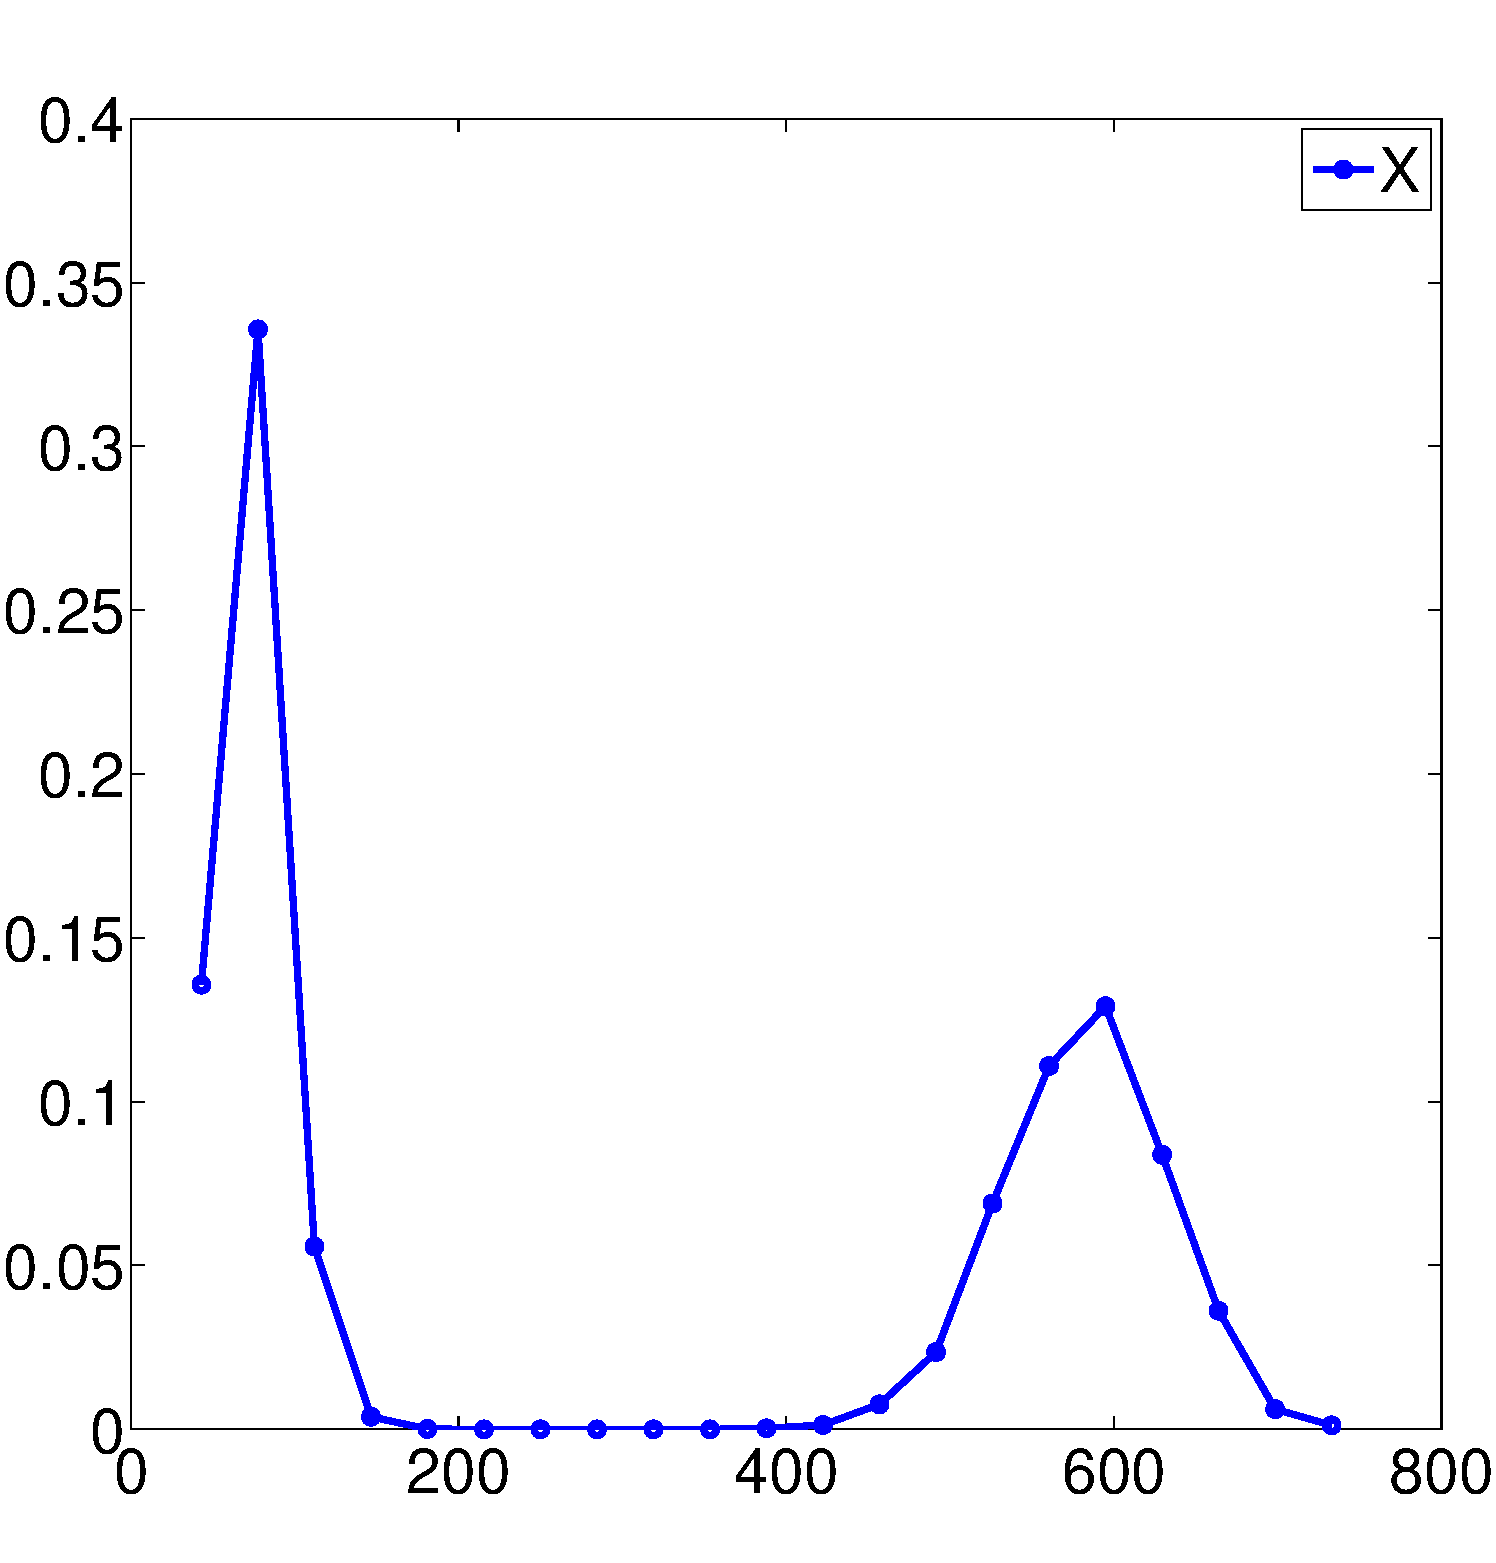
\includegraphics[width=0.5\textwidth]{figures/Schlogl_tau_hist.pdf}
			}
		\centerline{
			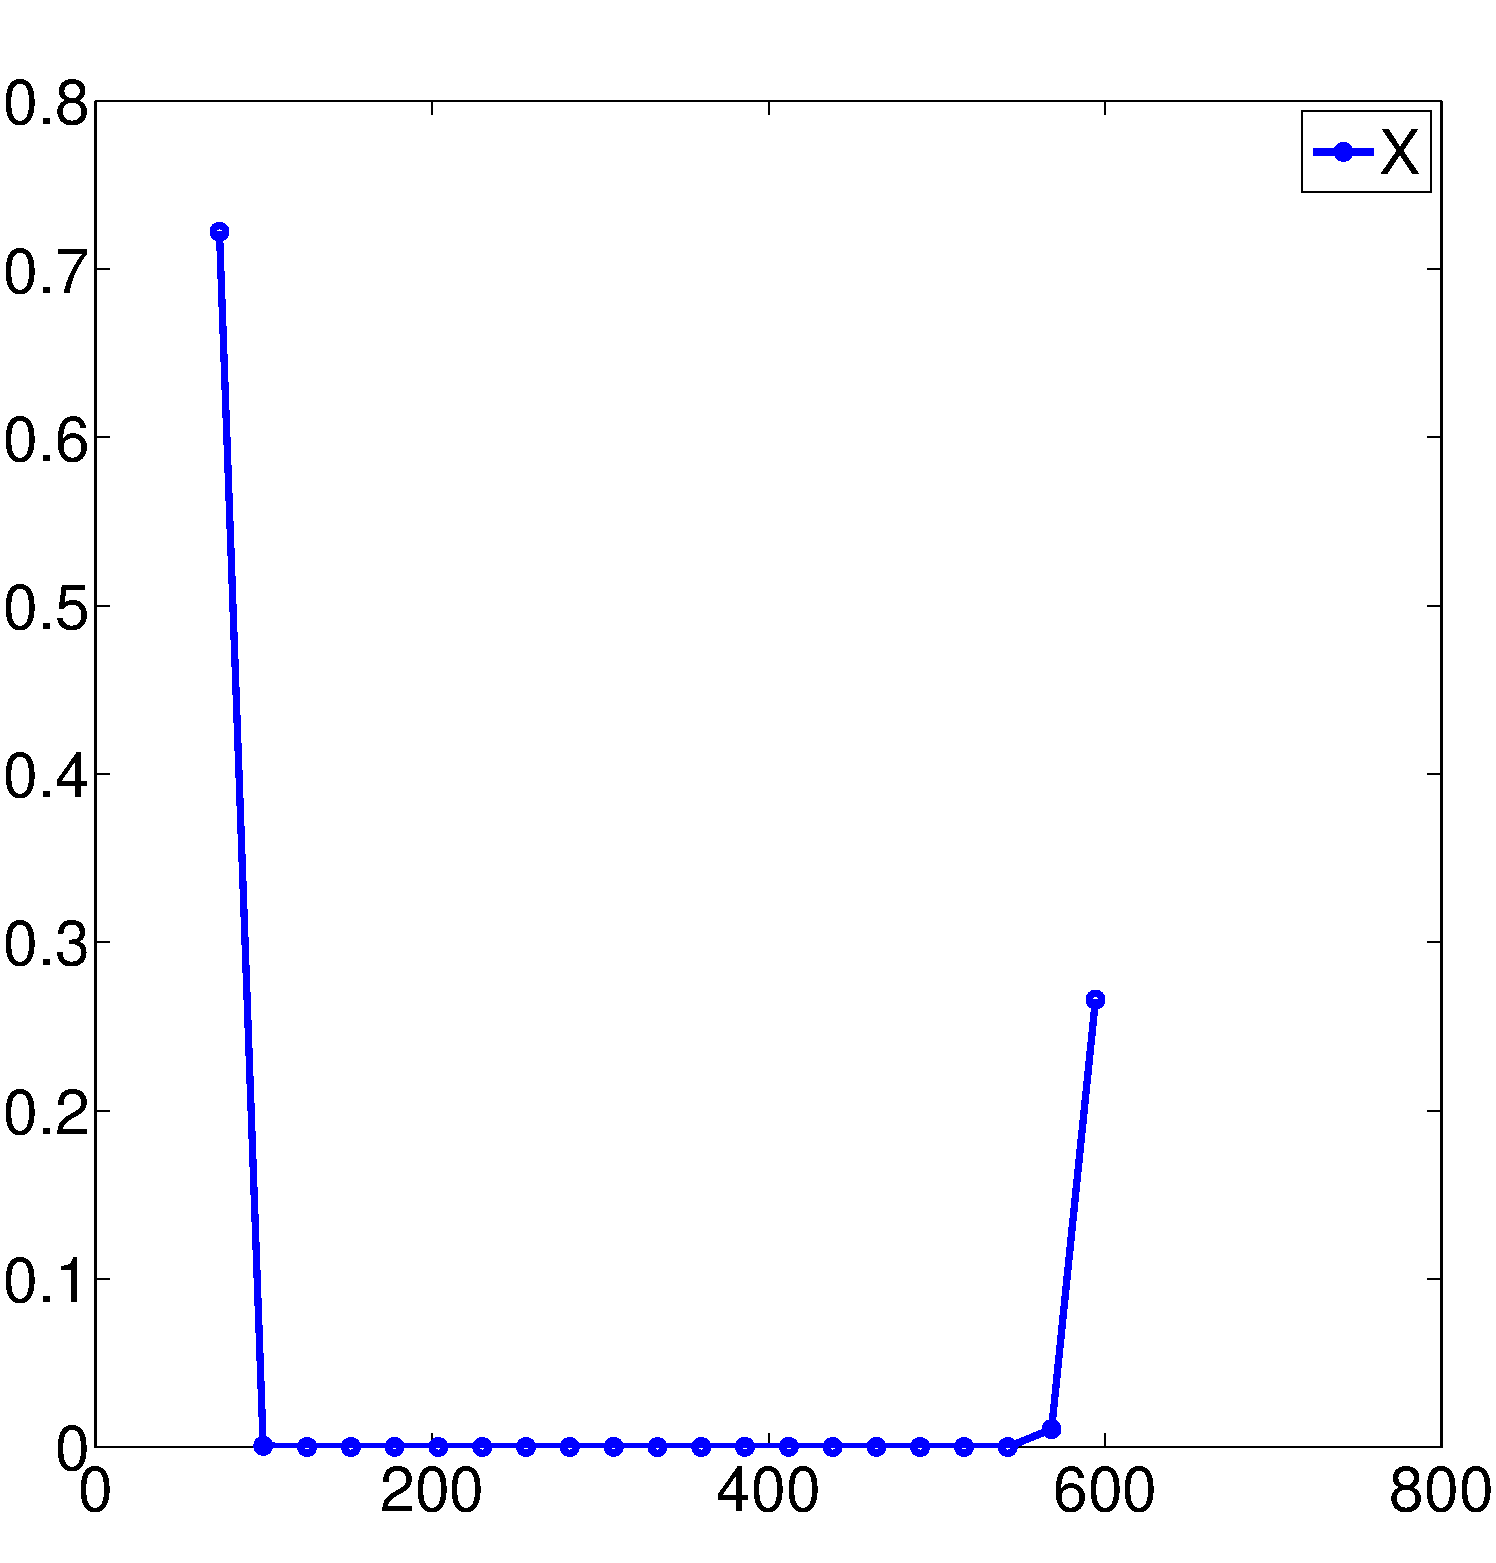
\includegraphics[width=0.5\textwidth]{figures/Schlogl_cle_hist.pdf}
			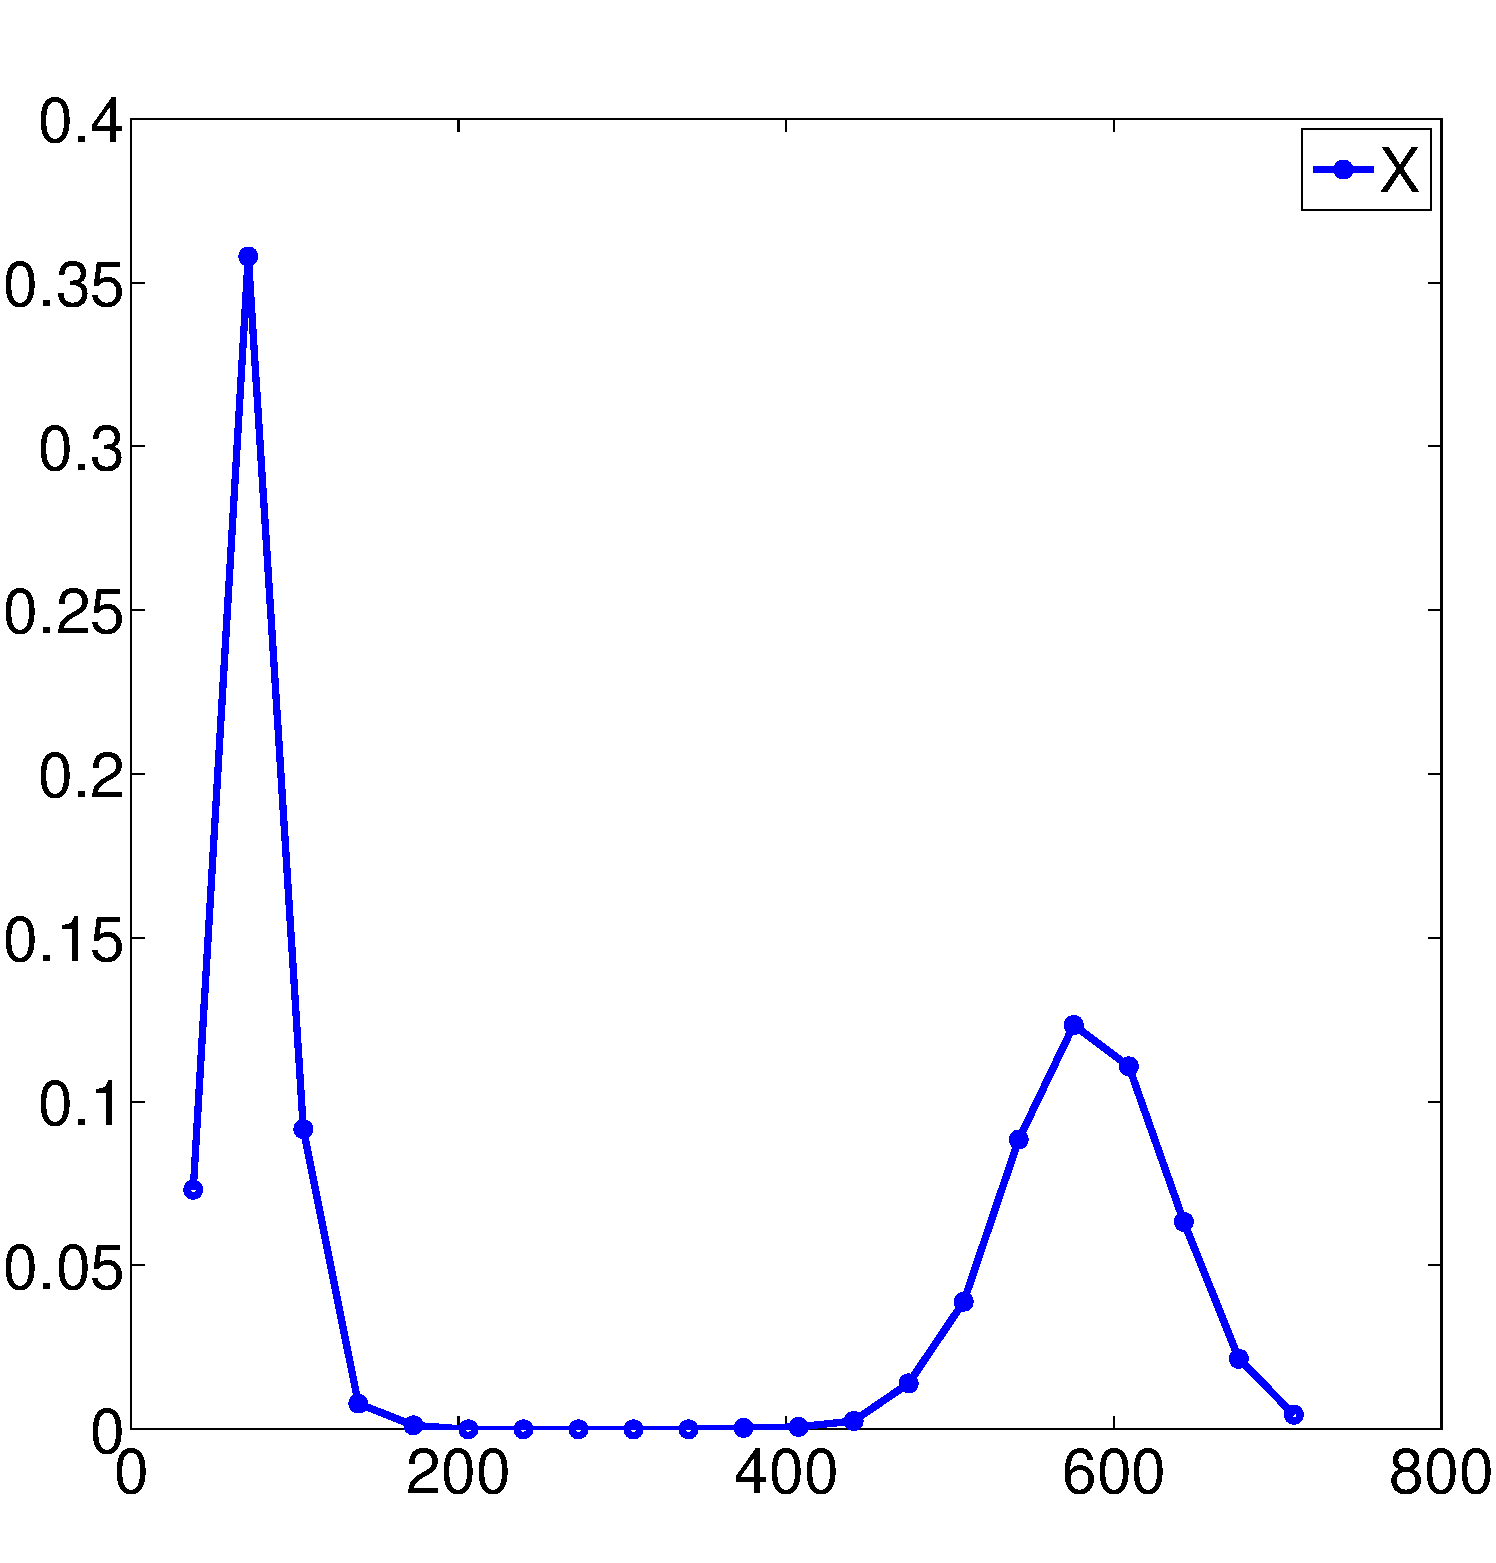
\includegraphics[width=0.5\textwidth]{figures/Schlogl_gpu_hist.pdf}
			}
		\captionsetup{width=0.8\textwidth}
		\caption[Histogram of end populations of the Schl\"{o}gl model from 10,000 trajectories]{Histogram of population amounts of 10,000 trajectories at the final time $T=15$, after simulation of the Schl\"{o}gl model over $[0,15]$ using SSA (top left), tau-leaping (top right), LLA/CLE (bottom left), and GPU (bottom right). The vertical axis shows frequency, the horizontal axis shows final population amounts. The value of $\tau$ utilized by tau-leaping and LLA/CLE was automatically determined by MARS.}
		\label{schlogl_hist_figure}
		\end{figure}

		\noindent
		Of note, the SSA, tau-leaping, LLA/CLE trajectory generations took about $3.11 \times 10^3$ s, $9.68 \times 10^2$ s, and $3.26 \times 10^2$ s, respectively, to complete, while the the GPU implementation took only about 6.46 s to complete. This represents a significant speedup of about {\bf 480} times over the SSA, {\bf 150} times over tau-leaping, and {\bf 50} times over LLA/CLE.

		\subsection{Varying the Initial Values in the Schl\"{o}gl Model}

			The aforementioned bifurcation behaviour exhibited by the Schl\"{o}gl model is responsible for the bimodal distribution seen in Figure \ref{schlogl_hist_figure}. This behaviour can most clearly be seen in Figure \ref{schlogl_comparison}.

			\begin{figure}[H]
			\centerline{
				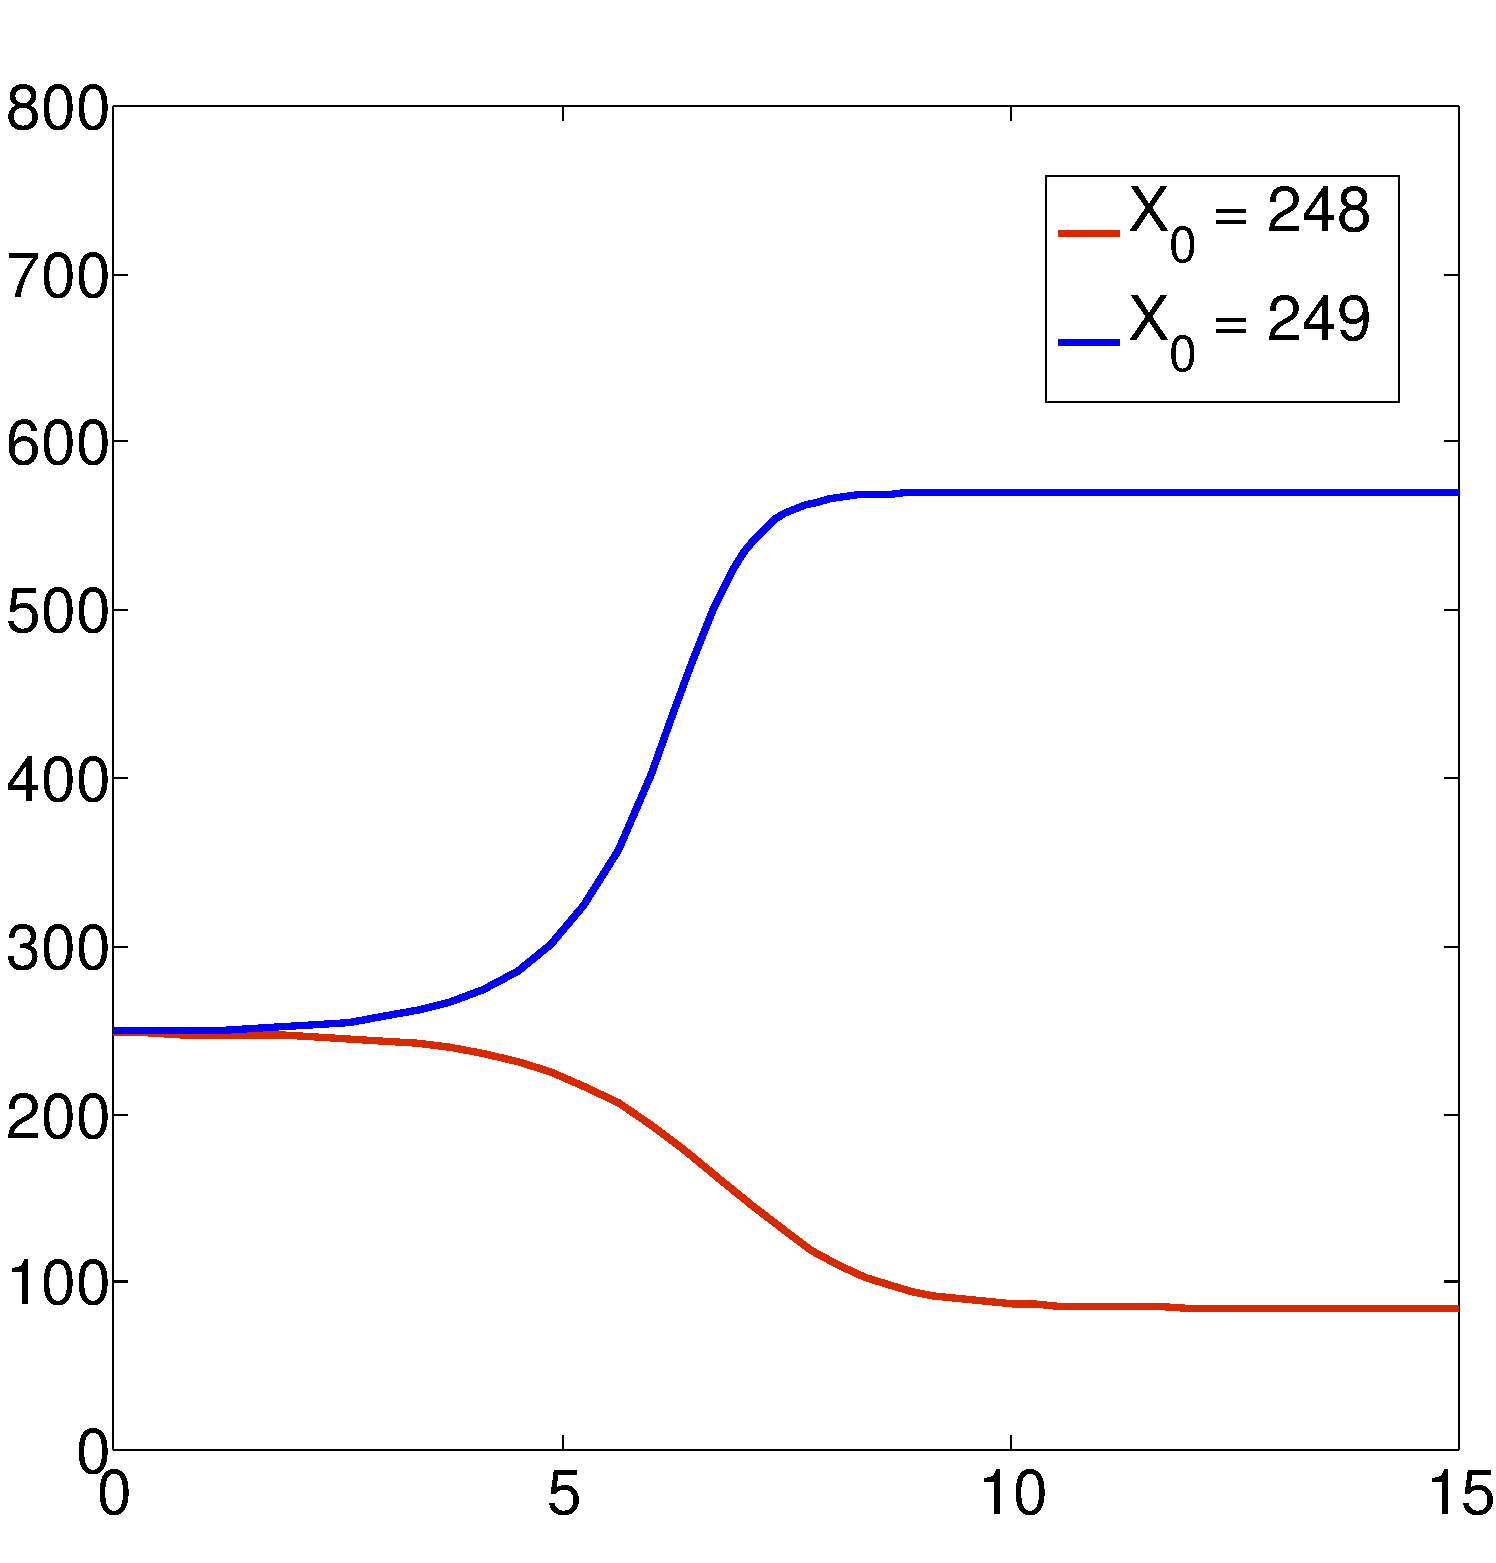
\includegraphics[width=0.5\textwidth]{figures/Schlogl_comp_rre.pdf}
				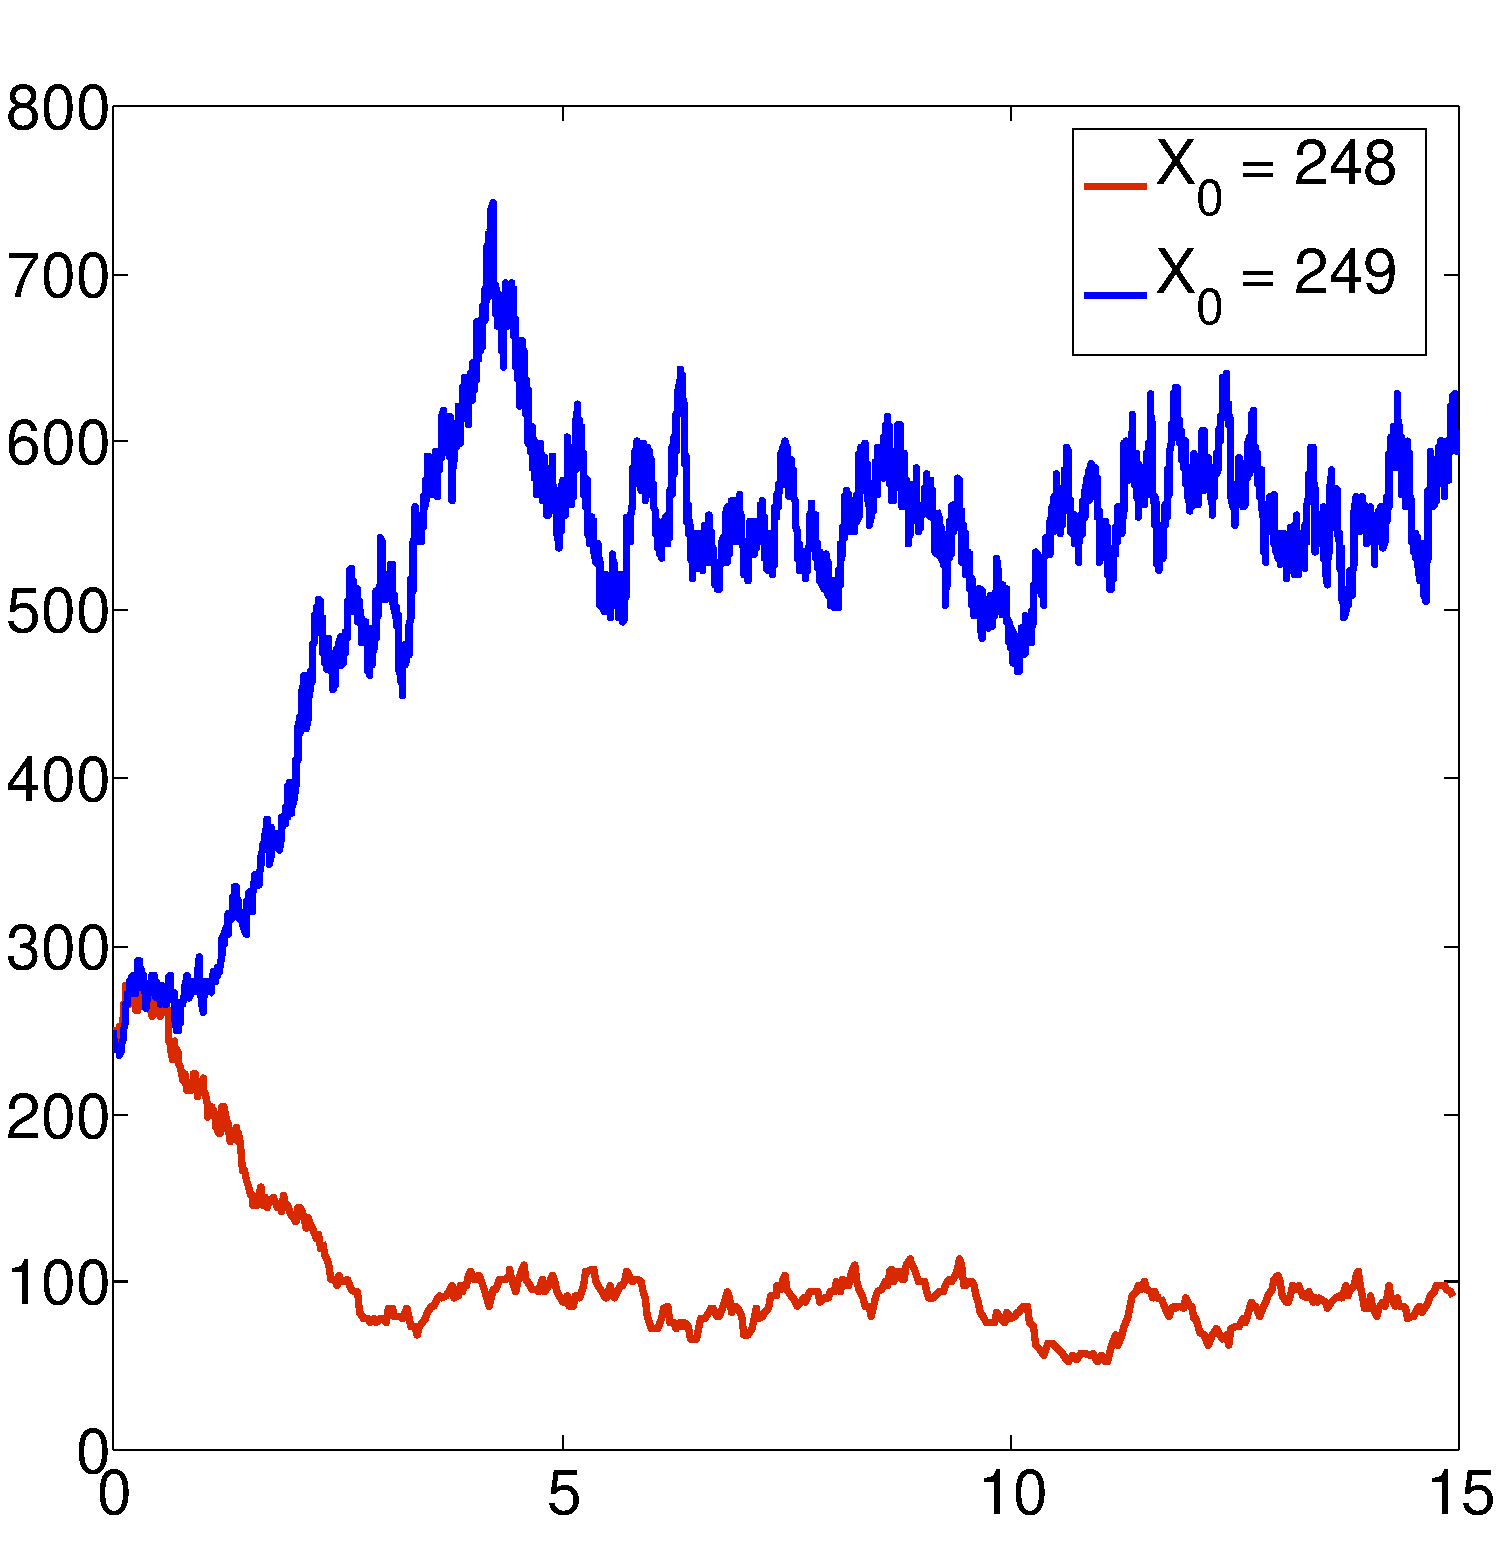
\includegraphics[width=0.5\textwidth]{figures/Schlogl_comp_ssa.pdf}
				}
			\captionsetup{width=0.8\textwidth}
			\caption[Resulting populations in the Schl\"{o}gl model with varying initial conditions]{Population of species $X$ in the Schl\"{o}gl model over $[0,15]$ with initial population set to 248 (bottom curve) or 249 (top curve). The right graph was generated using RRE and the, left using SSA for the CME.}
			\label{schlogl_comparison}
			\end{figure}

	\section{Multilevel Monte Carlo Tau-leaping}

		The accuracy of the MLMC method, and the speedup obtained, as compared with the simulating of 10,000 trajectories using SSA were determined by direct comparison on three biochemical systems of interest. In each case, the M-value required by MLMC was determined through a mix of systematic testing and trial-and-error. It should be noted that the accuracy and the speed of the MLMC method is highly dependant on both this parameter and the tolerance specified by the user. An error of $10^{-2}$ and an M-value of 5 typically produced the best results.

		\subsection{Goldbeter-Koshland Switch}

			The Goldbeter-Koshland Switch model \cite{chem_phys_models} consists of six species engaged in two reversible reactions (which are split into four reactions), and two non-reversible reactions. It models a phosphorylation-dephosphorylation system containing two enzymes, $E_1$ and $E_2$.\\
			\\
			The relevant model data is summarized in Table \ref{gks_table}.

			\begin{table}[H]
			\[
			\begin{array}{l@{\hspace*{10mm}}r@{\ }c@{\ }l@{\hspace*{10mm}}l@{\hspace*{10mm}}l}
			\multicolumn{4}{c}{\text{{\huge\phantom{$I_{I_I}$}}Reactions}} & \multicolumn{1}{c}{\text{Propensities}} & \multicolumn{1}{c}{\text{Reaction rates}}\\
			\hline
			R_1 	& S + E_1 & \stackrel{c_1}{\rightarrow} & C_1 	& a_1(\mathbf{x}) = c_1 S E_1 	& c_1 = 0.05
			\\\\
			R_2 	& C_1 & \stackrel{c_2}{\rightarrow} & S + E_1  	& a_2(\mathbf{x}) = c_2 C_1		& c_2 = 0.1
			\\\\
			R_3 	& C_1 & \stackrel{c_3}{\rightarrow} & P + E_1 	& a_3(\mathbf{x}) = c_3 C_1		& c_3 = 0.1
			\\\\
			R_4 	& P + E_2 & \stackrel{c_4}{\rightarrow} & C_2 	& a_4(\mathbf{x}) = c_4 P E_2	& c_4 = 0.01
			\\\\
			R_5 	& C_2 & \stackrel{c_5}{\rightarrow} & P + E_2 	& a_5(\mathbf{x}) = c_5 C_2		& c_5 = 0.1
			\\\\
			R_6 	& C_2 & \stackrel{c_6}{\rightarrow} & S + E_2 	& a_6(\mathbf{x}) = c_6 C_2		& c_6 = 0.1
			\end{array}
			\]
			\captionsetup{width=0.8\textwidth}
			\caption{Goldbeter-Koshland Switch model}
			\label{gks_table}
			\end{table}

			\noindent
			The model was integrated with with initial population values for $(S,E_1,C_1,P,E_2,C_2)^T$ of $(110,100,30,\\30,100,30)^T$. The MLMC algorithm was implemented with an M-value of 5 and a tolerance of $10^{-2}$, requiring 20 single coarse trajectories at level $l_0$, and 100, 20 coupled trajectories at levels $l_0/l_1,l_1/L$ respectively. SSA was utilized to generate 10,000 trajectories, with average population values taken at 100 steps over the integration. The integration interval was $[0,5]$.\\
			\\
			We show the numerical results in Figure \ref{gks_mlmc}.

			\begin{figure}[H]
			\centerline{
				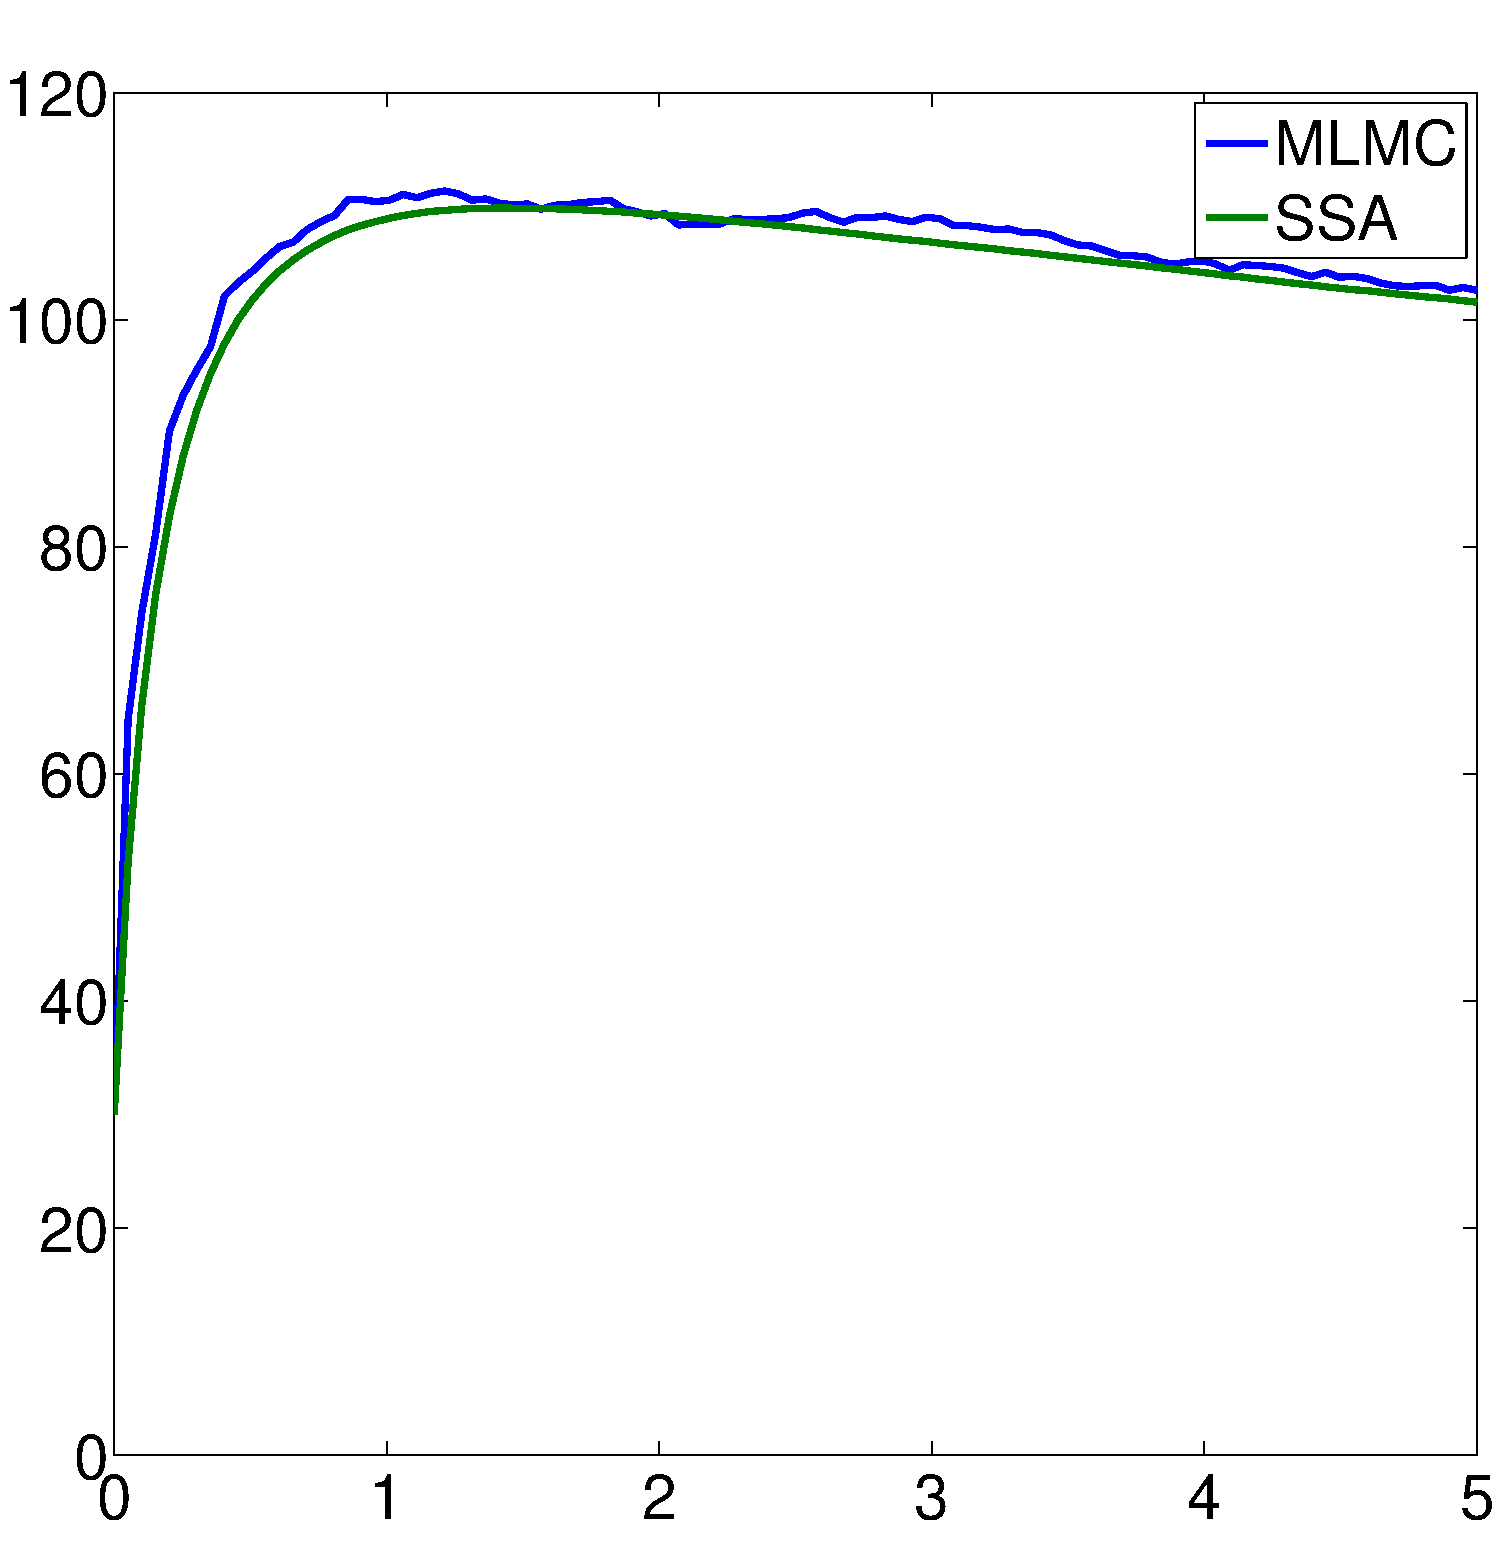
\includegraphics[width=0.5\textwidth]{figures/GKS_c1_mlmc.pdf}
				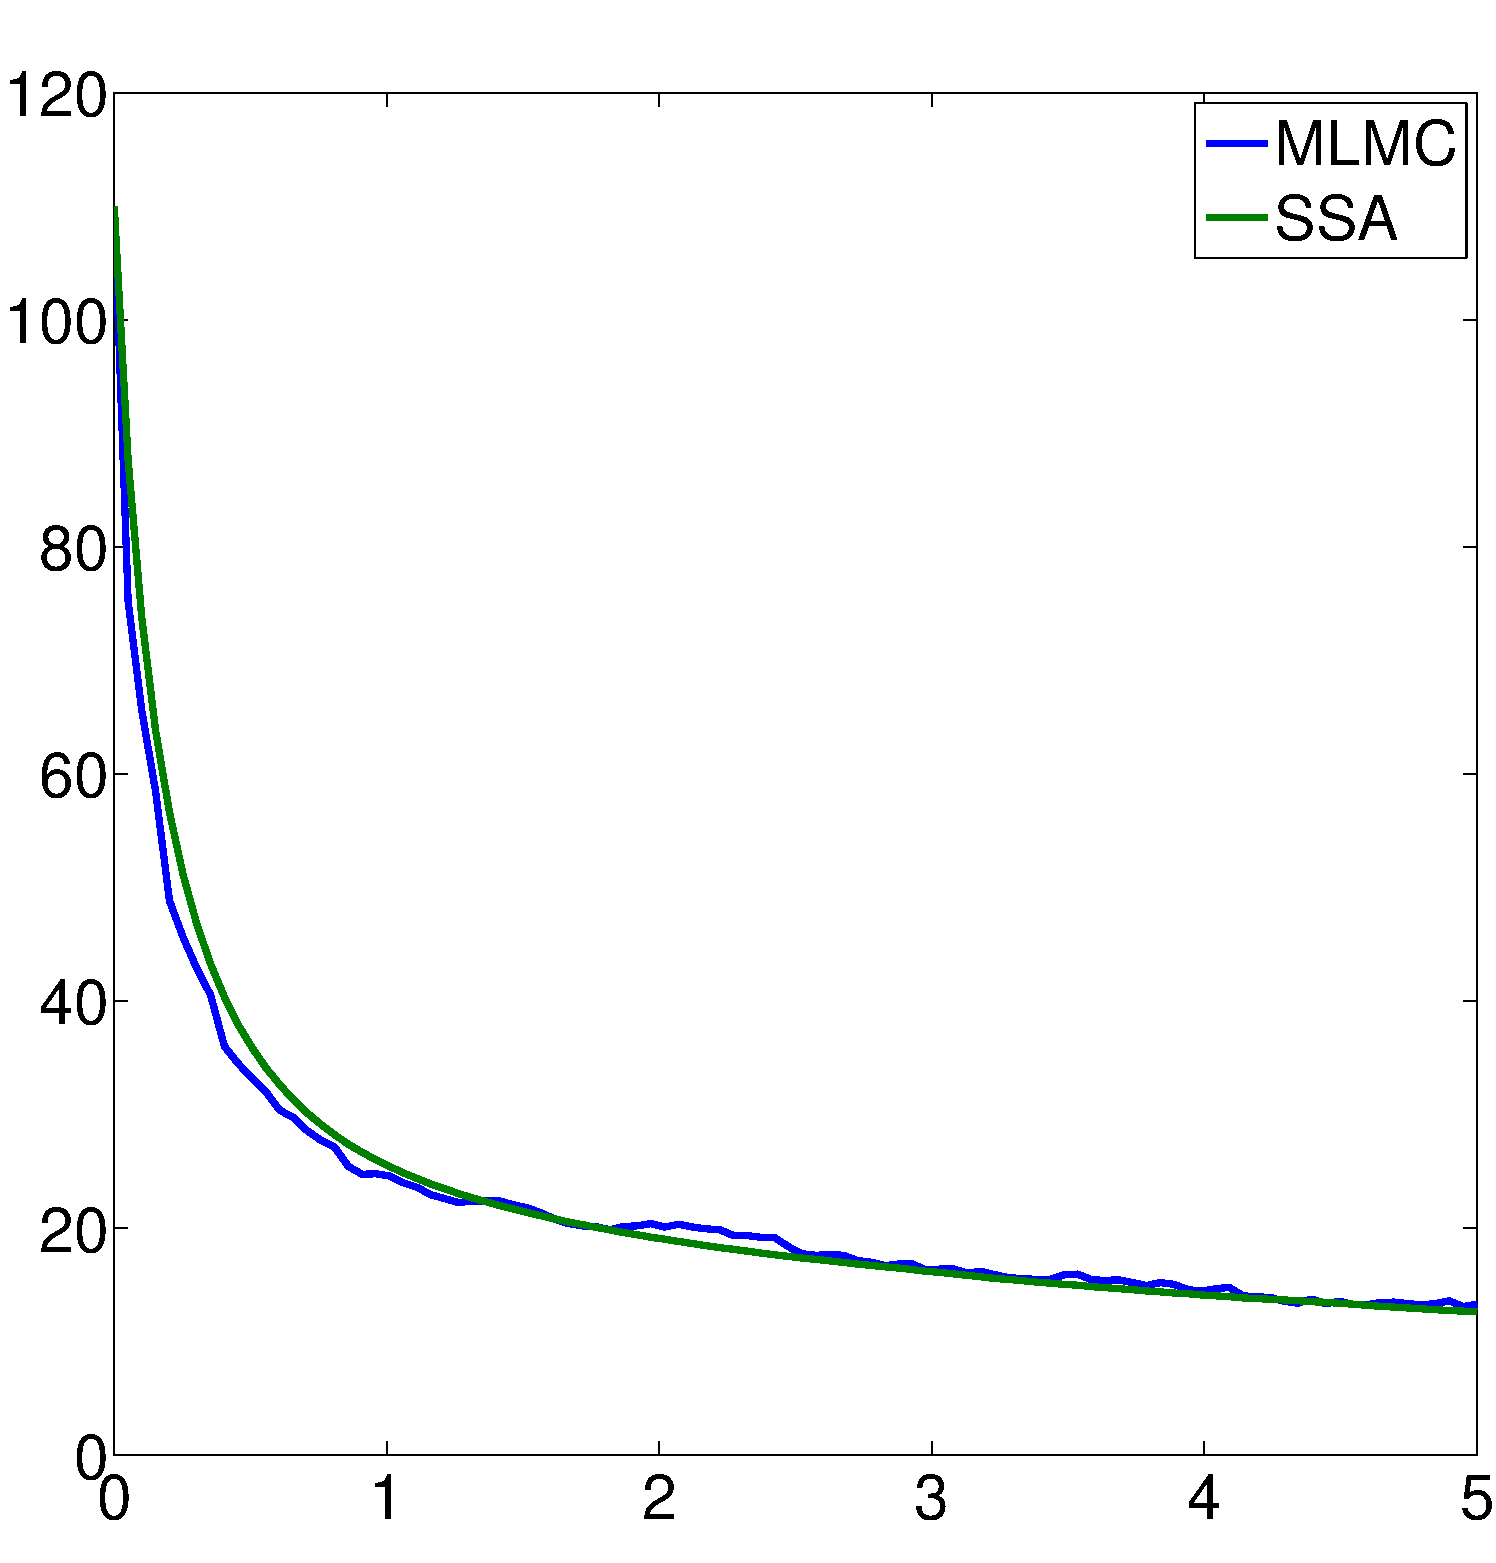
\includegraphics[width=0.5\textwidth]{figures/GKS_s_mlmc.pdf}
				}
			\centerline{
				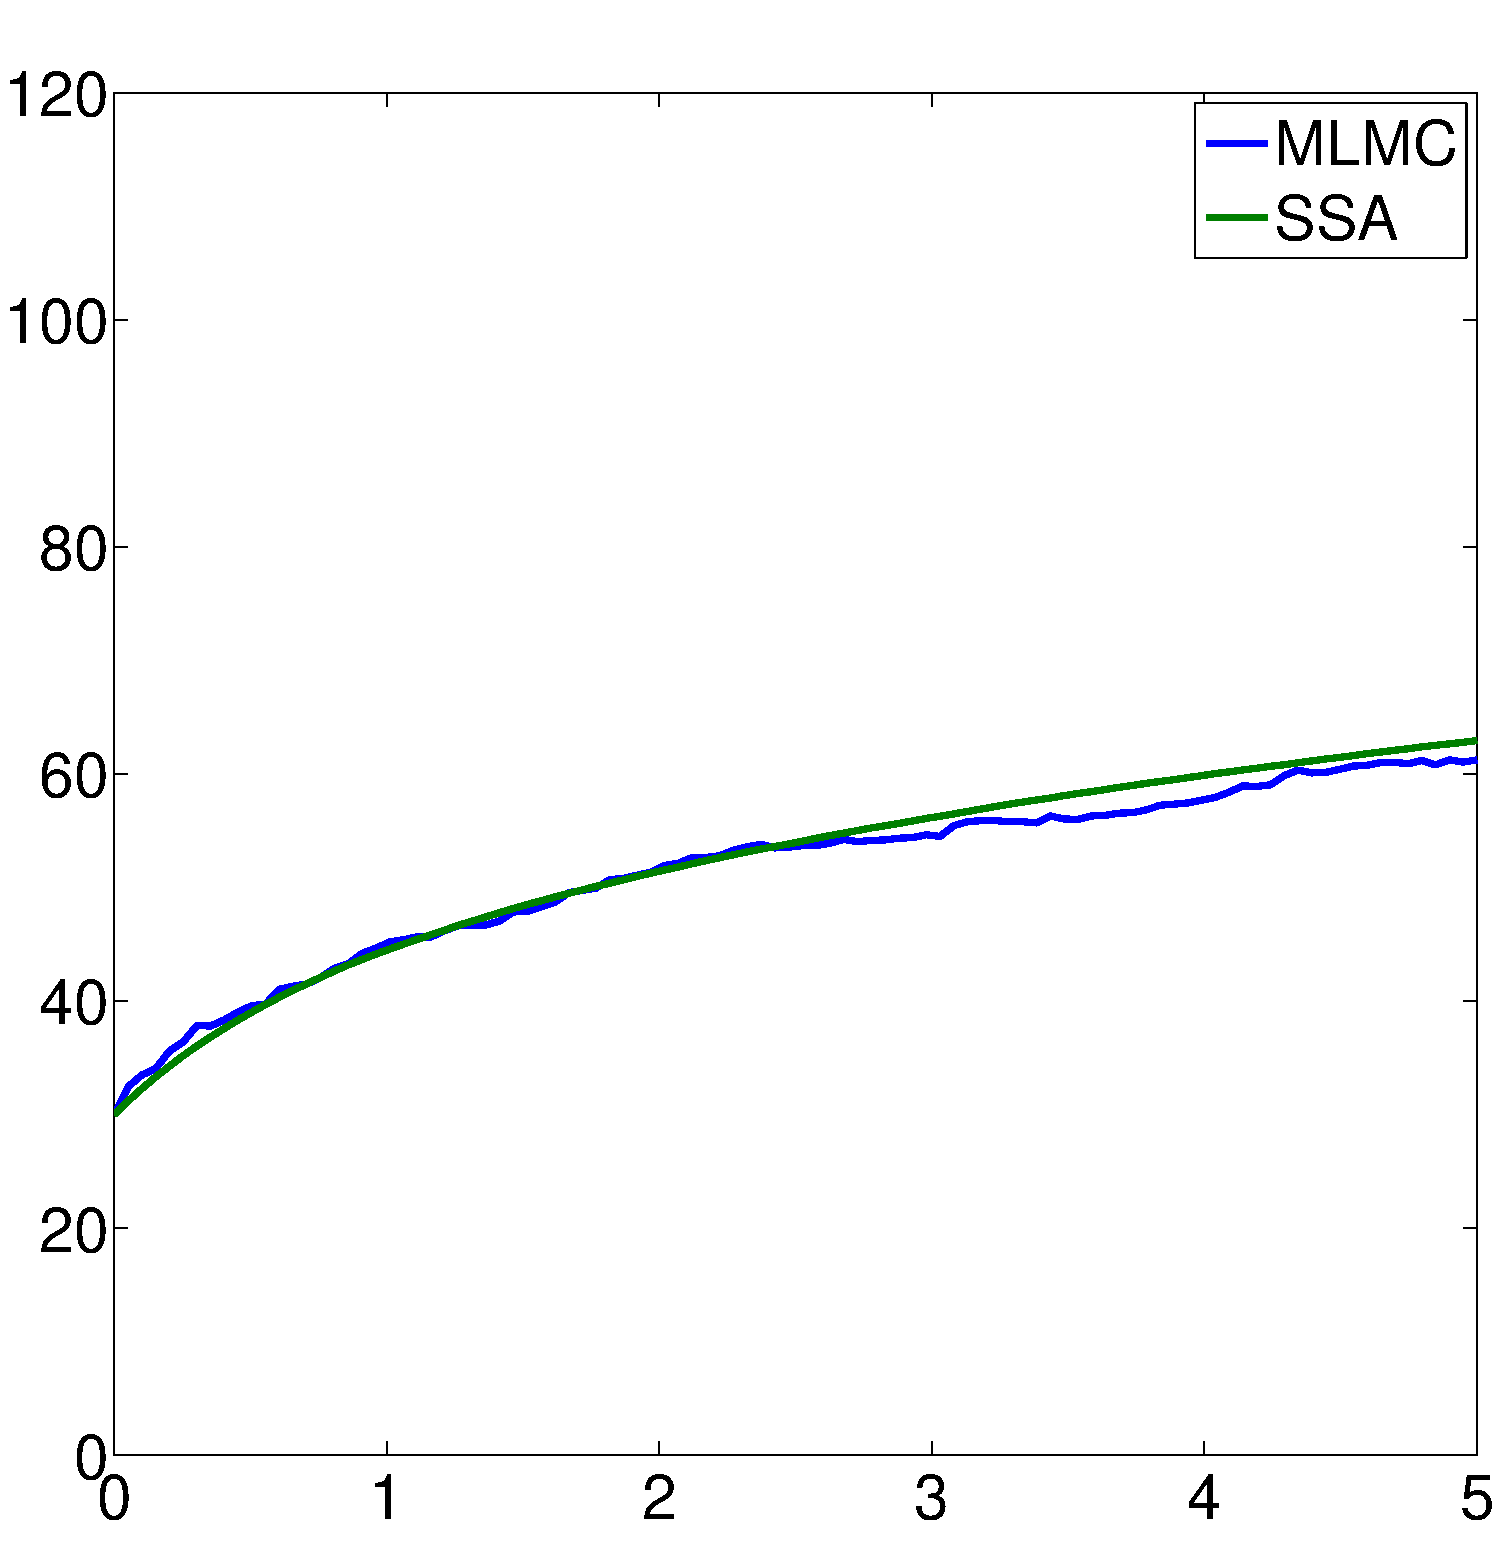
\includegraphics[width=0.5\textwidth]{figures/GKS_c2_mlmc.pdf}
				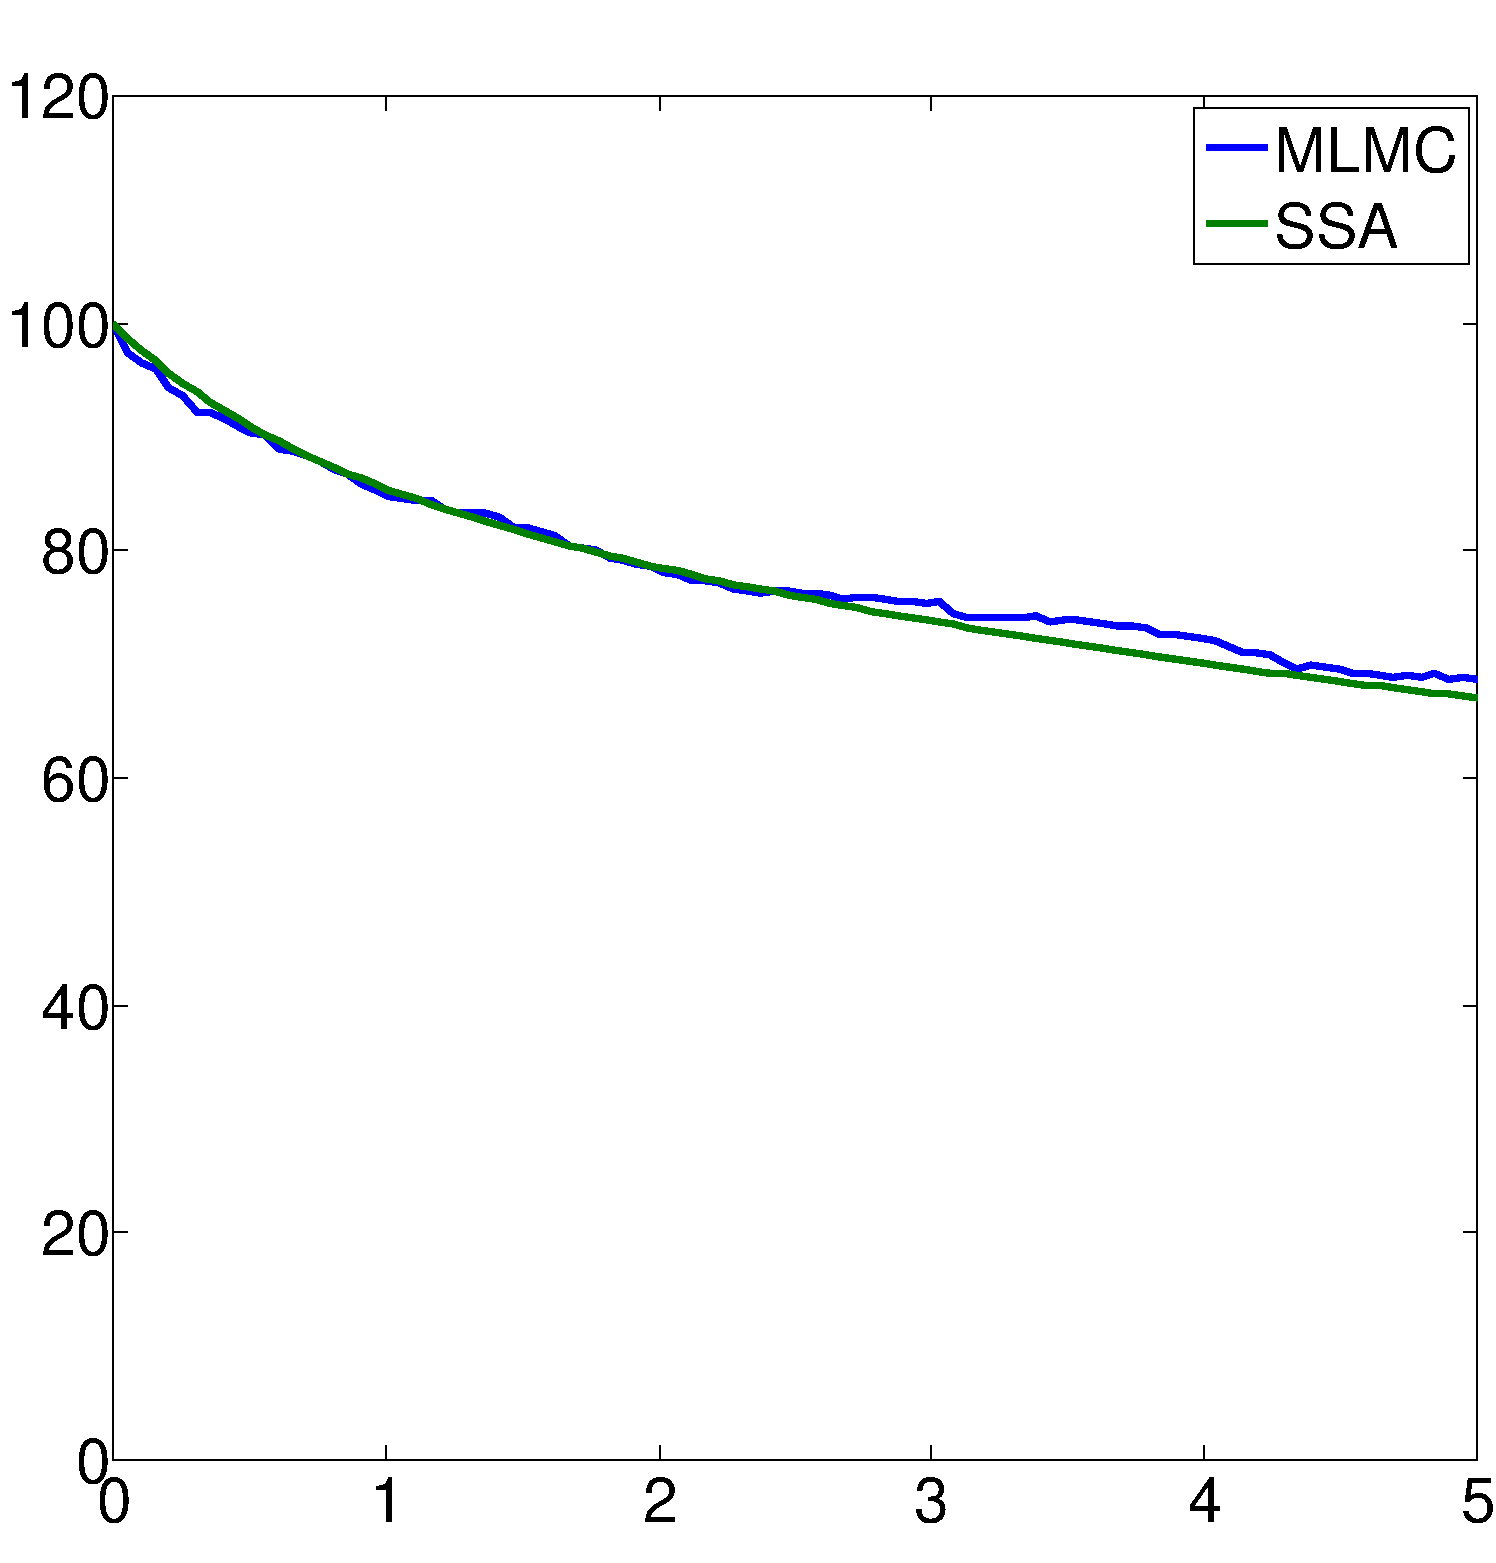
\includegraphics[width=0.5\textwidth]{figures/GKS_e2_mlmc.pdf}
				}
			\captionsetup{width=0.8\textwidth}
			\caption[Estimated average population values for species in Goldbeter-Koshland Switch using MLMC compared to 10,000 SSA trajectories over {$[0,5]$}]{Estimated average populations for the species in the Goldbeter-Koshland Switch model computed using the MLMC method compared to the average population values taken from 10,000 trajectories generated by the SSA. The results are presented for species $C_1$ (top left), $S$ (top right), $C_2$ (bottom left), and $E_2$ (bottom right). The vertical axis shows population amounts, while the horizontal axis shows simulation time. Integration was taken over $[0,5]$.}
			\label{gks_mlmc}
			\end{figure}
			
			\noindent
			In addition to the MLMC plots visually showing an excellent agreement with the predictions of the exact SSA strategy, the method took about 2.55 seconds to complete, while the 10,000 SSA trajectories took about 21.19 seconds. This represents a 8.31 times speedup. The precise errors from the final population values, are given in the Table \ref{gks_error}.

			\begin{table}[H]
			\centering
			\begin{tabular}{ >{$}l<{$} >{$}l<{$} >{$}l<{$}}
				\text{Species} 	& \text{Absolute error}	& \text{Relative error} \\
				\hline
				S 			& 6.55 \times 10^{-1} 		& 5.18 \times 10^{-2} \\
				E_1			& 1.05 		 				& 3.67 \times 10^{-2} \\
				C_1 		& 1.05 		 				& 1.03 \times 10^{-2} \\
				P  			& 1.44 \times 10^{-2}		& 6.30 \times 10^{-4} \\
				E_2 		& 1.69 						& 2.51 \times 10^{-2} \\
				C_2 		& 1.69					 	& 2.68 \times 10^{-2} \\
			\end{tabular}
			\captionsetup{width=0.8\textwidth}
			\caption{Errors for the estimated species populations in the Goldbeter-Koshland Switch model using the MLMC method compared to 10,000 SSA trajectories}
			\label{gks_error}
			\end{table}
		
		\subsection{Cyclical Reaction System}

			The cyclical reaction system model \cite{chem_phys_models} consists of three species engaged three non-reversible reactions, forming a loop.\\
			\\
			The relevant model data is presented in Table \ref{crs_table}:

			\begin{table}[H]
			\[
			\begin{array}{l@{\hspace*{10mm}}r@{\ }c@{\ }l@{\hspace*{10mm}}l@{\hspace*{10mm}}l}
			\multicolumn{4}{c}{\text{{\huge\phantom{$I_{I_I}$}}Reactions}} & \multicolumn{1}{c}{\text{Propensities}} & \multicolumn{1}{c}{\text{Reaction rates}}\\
			\hline
			R_1 	& A_1 & \stackrel{c_1}{\rightarrow} & A_2 		& a_1(\mathbf{x}) = c_1 A_1 	& c_1 = 0.1
			\\\\
			R_2 	& A_2 & \stackrel{c_2}{\rightarrow} & A_3 		& a_2(\mathbf{x}) = c_2 A_2 	& c_2 = 0.1
			\\\\
			R_3 	& A_3 & \stackrel{c_3}{\rightarrow} & A_1 		& a_3(\mathbf{x}) = c_3 A_3 	& c_3 = 0.1
			\end{array}
			\]
			\captionsetup{width=0.8\textwidth}
			\caption{Cyclical Reaction System model}
			\label{crs_table}
			\end{table}

			\noindent
			The initial population values for $(A_1,A_2,A_3)^T$ are $(100,80,100)^T$. The MLMC algorithm was implemented with an M-value of 5 and a tolerance of $10^{-2}$, requiring 1000 single coarse trajectories at level $l_0$, and 4, 4 coupled trajectories at levels $l_0/l_1,l_1/L$ respectively. The SSA was employed to simulate 10,000 trajectories, with average population values taken at 100 steps over the integration interval. The integration was performed over the time interval $[0,20]$.\\
			\\
			The numerical results are in Figure \ref{crs_mlmc}:

			\begin{figure}[H]
			\centerline{
				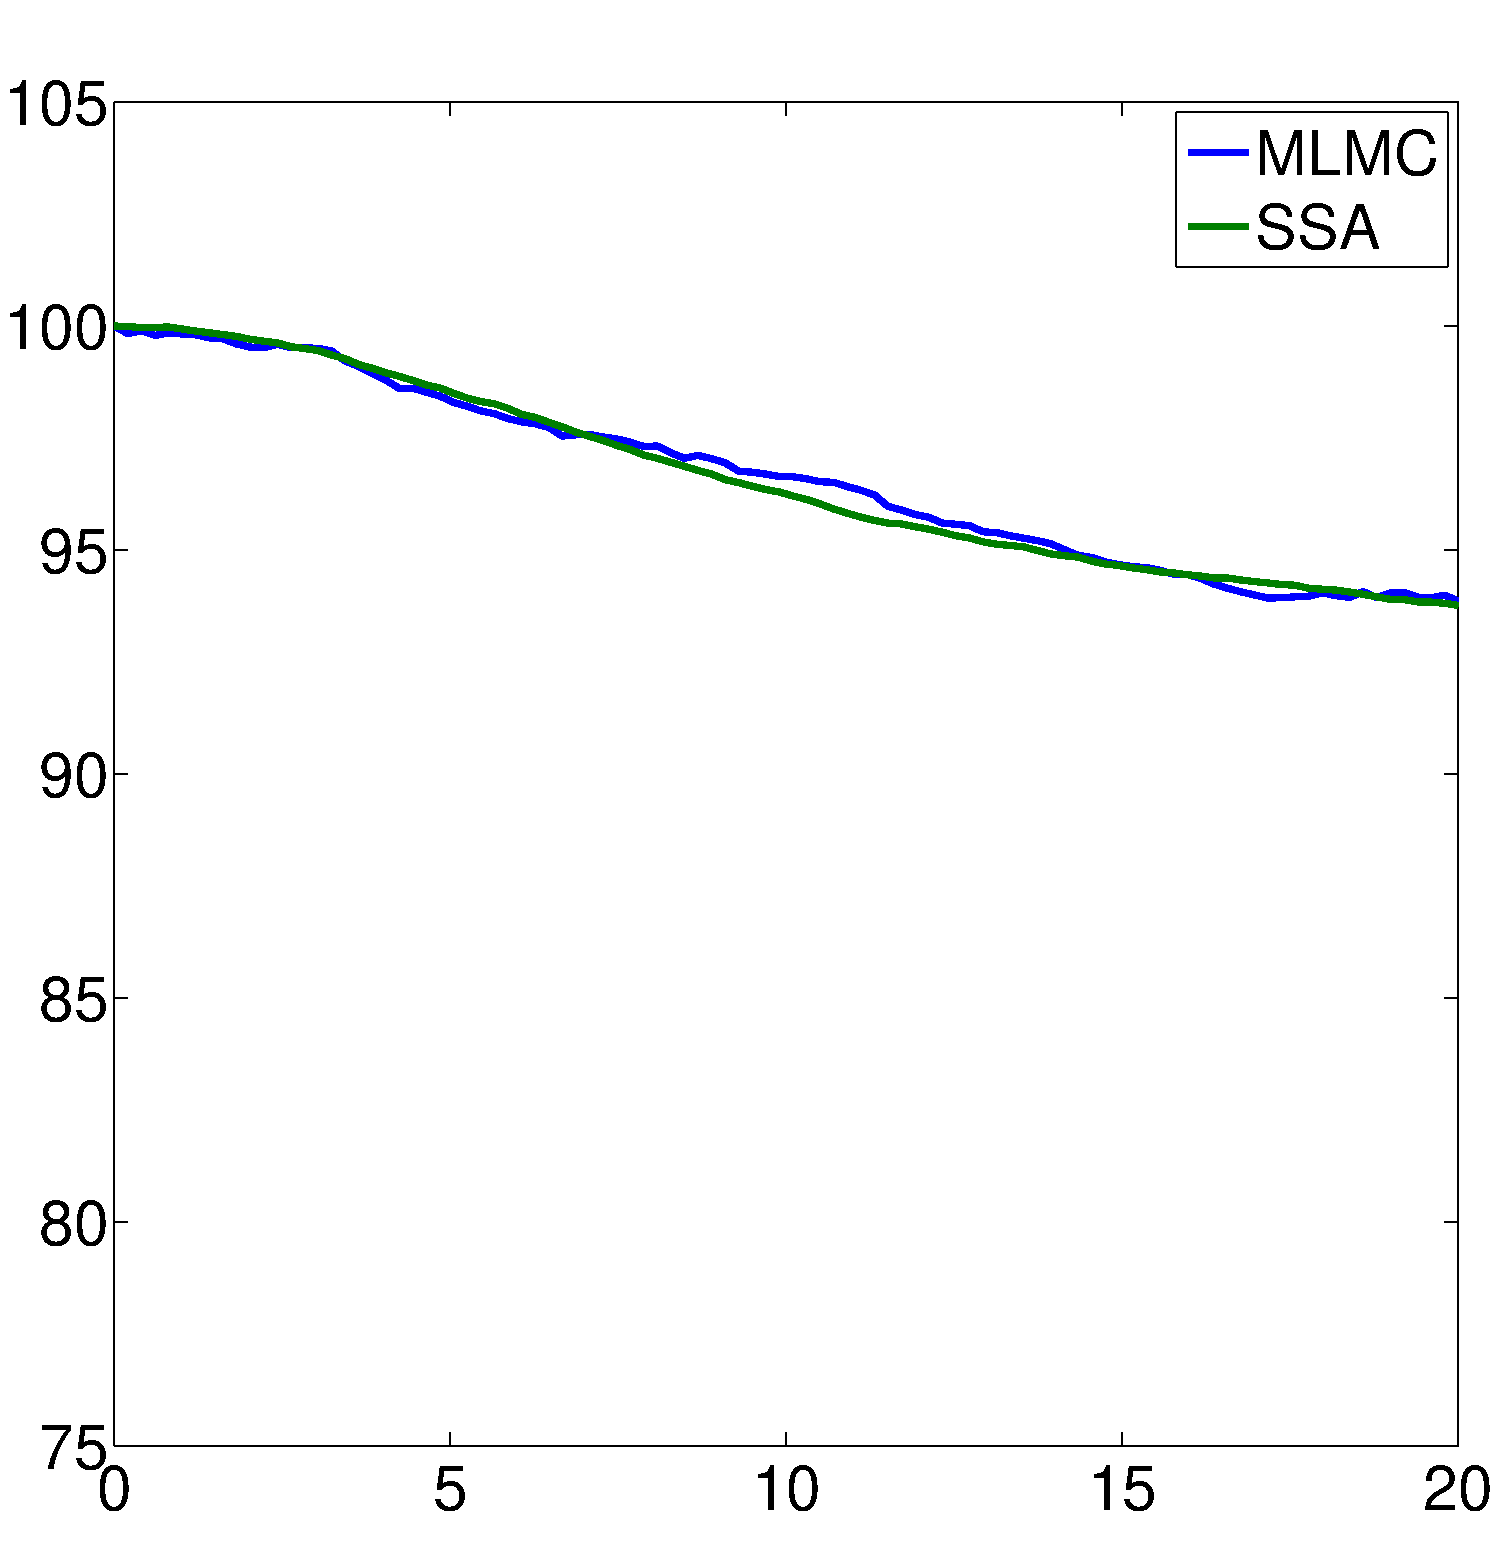
\includegraphics[width=0.5\textwidth]{figures/CRS_a1_mlmc.pdf}
				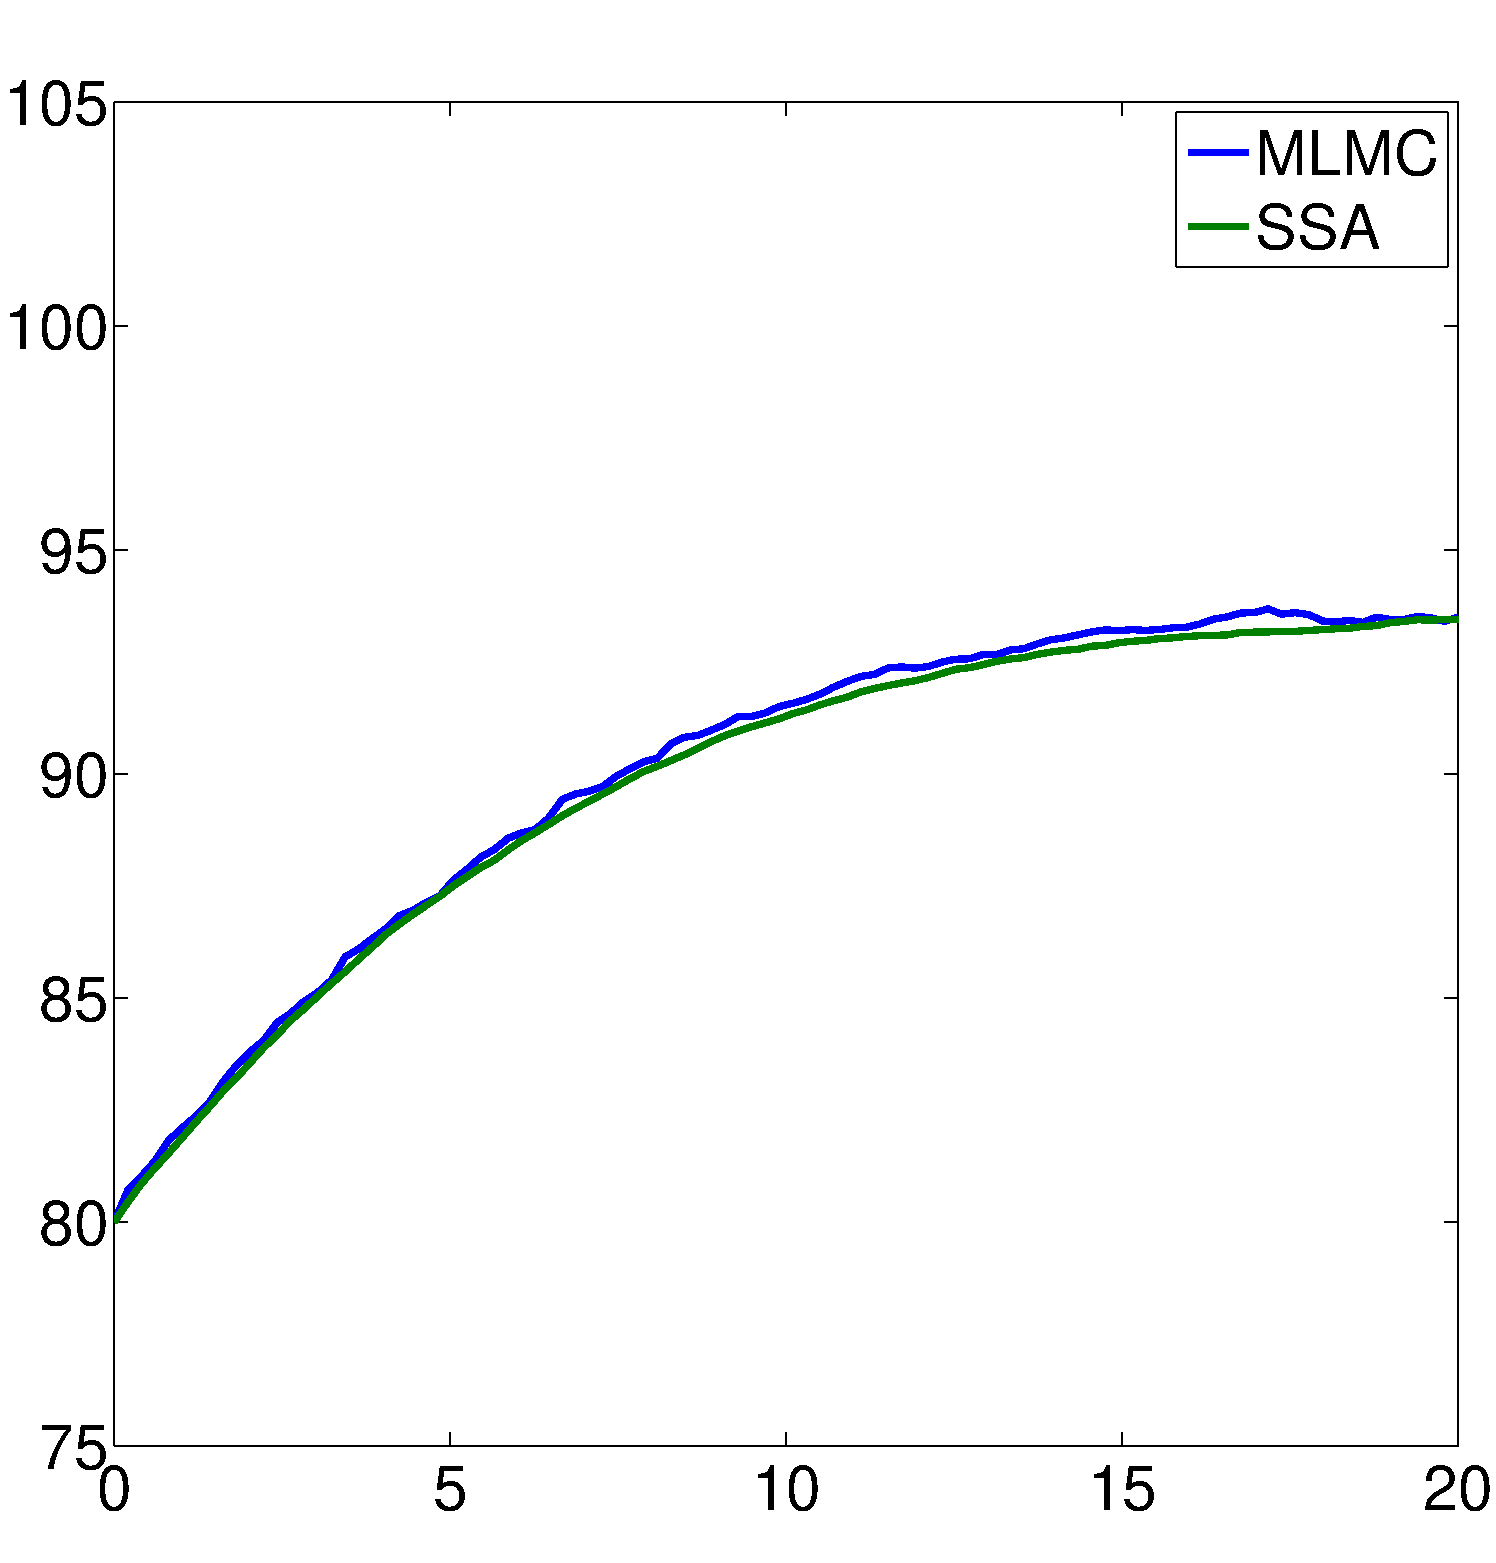
\includegraphics[width=0.5\textwidth]{figures/CRS_a2_mlmc.pdf}
				}
			\captionsetup{width=0.8\textwidth}
			\caption[Estimated average population values for species in Cyclical Reaction System using MLMC compared to 10,000 SSA trajectories  over {$[0,20]$}]{Evolution of the estimated average populations for species in the cyclical reaction system computed using MLMC compared to that for the average population values taken from 10,000 trajectories generated with the SSA. The results are for the species $A_1$ (left), $A_2$ (right). The vertical axis shows population amounts, while the horizontal axis shows simulation time. Integration was taken over $[0,20]$.}
			\label{crs_mlmc}
			\end{figure}
			
			\noindent
			We remark that the MLMC plots again show an excellent agreement with the results obtained for the 10,000 SSA trajectories. In addition the method took about 2.59 seconds to complete, while the 10,000 SSA trajectories took about 25.85 seconds. This represents a 9.98 times speedup. The precise errors from the final population values are in Table \ref{crs_error}.

			\begin{table}[H]
			\centering
			\begin{tabular}{ >{$}l<{$} >{$}l<{$} >{$}l<{$}}
				\text{Species} 	& \text{Absolute error}	& \text{Relative error} \\
				\hline
				A_1 		& 9.86 \times 10^{-2}		& 1.05 \times 10^{-3} \\
				A_2			& 4.89 \times 10^{-2}		& 5.23 \times 10^{-4} \\
				A_3 		& 1.48 \times 10^{-1}		& 1.59 \times 10^{-3} \\
			\end{tabular}
			\captionsetup{width=0.8\textwidth}
			\caption{Errors for the estimated species populations in the cyclical reaction system model using MLMC compared to 10,000 SSA trajectories}
			\label{crs_error}
			\end{table}

		\subsection{Potassium Channel}

			The Potassium Channel model \cite{chem_phys_models} consists of five species subject to 5 reversible reactions (which are split into 10 simple reactions). Three species represent separate closed states, one species is an open state, and the last is an inactivation state.\\
			\\
			The relevant model data is included in Table \ref{pc_table}:

			\begin{table}[H]
			\[
			\begin{array}{l@{\hspace*{10mm}}r@{\ }c@{\ }l@{\hspace*{10mm}}l@{\hspace*{10mm}}l}
			\multicolumn{4}{c}{\text{{\huge\phantom{$I_{I_I}$}}Reactions}} & \multicolumn{1}{c}{\text{Propensities}} & \multicolumn{1}{c}{\text{Reaction rates}}\\
			\hline
			R_1 	& C_1 & \stackrel{c_1}{\rightarrow} & C_2 	& a_1(\mathbf{x}) = c_1 S C_1 	& c_1 = 0.1
			\\\\
			R_2 	& C_2 & \stackrel{c_2}{\rightarrow} & C_1  	& a_2(\mathbf{x}) = c_2 C_2		& c_2 = 0.1
			\\\\
			R_3 	& C_2 & \stackrel{c_3}{\rightarrow} & C_3 	& a_3(\mathbf{x}) = c_3 C_2		& c_3 = 0.1
			\\\\
			R_4 	& C_3 & \stackrel{c_4}{\rightarrow} & C_2 	& a_4(\mathbf{x}) = c_4 C_3		& c_4 = 0.1
			\\\\
			R_5 	& C_3 & \stackrel{c_5}{\rightarrow} & O 	& a_5(\mathbf{x}) = c_5 C_3		& c_5 = 0.1
			\\\\
			R_6 	& O & \stackrel{c_6}{\rightarrow} & C_3 	& a_6(\mathbf{x}) = c_6 O		& c_6 = 0.1
			\\\\
			R_7 	& O & \stackrel{c_7}{\rightarrow} & I 		& a_7(\mathbf{x}) = c_7 C_2		& c_7 = 0.1
			\\\\
			R_8 	& I & \stackrel{c_8}{\rightarrow} & O 		& a_8(\mathbf{x}) = c_8 C_3		& c_8 = 0.1
			\\\\
			R_9 	& I & \stackrel{c_9}{\rightarrow} & C_3 	& a_9(\mathbf{x}) = c_9 C_3		& c_9 = 0.1
			\\\\
			R_{10} 	& C_3 & \stackrel{c_{10}}{\rightarrow} & I 	& a_{10}(\mathbf{x}) = c_{10} O	& c_{10} = 0.1
			\end{array}
			\]
			\captionsetup{width=0.8\textwidth}
			\caption{Potassium Channel model}
			\label{pc_table}
			\end{table}

			\noindent
			The initial population values for the species $(C_1,C_2,C_3,O,I)^T$ are $(100,50,100,50,\\100)^T$. The MLMC technique was implemented with an M-value of 5 and a tolerance of $10^{-2}$, requiring 1000 single coarse trajectories at level $l_0$, and 4, 4 coupled trajectories at levels $l_0/l_1,l_1/L$ respectively. SSA was applied to generate 10,000 trajectories, with average population values taken at 100 steps over the integration. The system was integrated over the time interval $[0,10]$.\\
			\\
			The results of our simulation using MARS are shown in Figure \ref{pc_mlmc}.

			\begin{figure}[H]
			\centerline{
				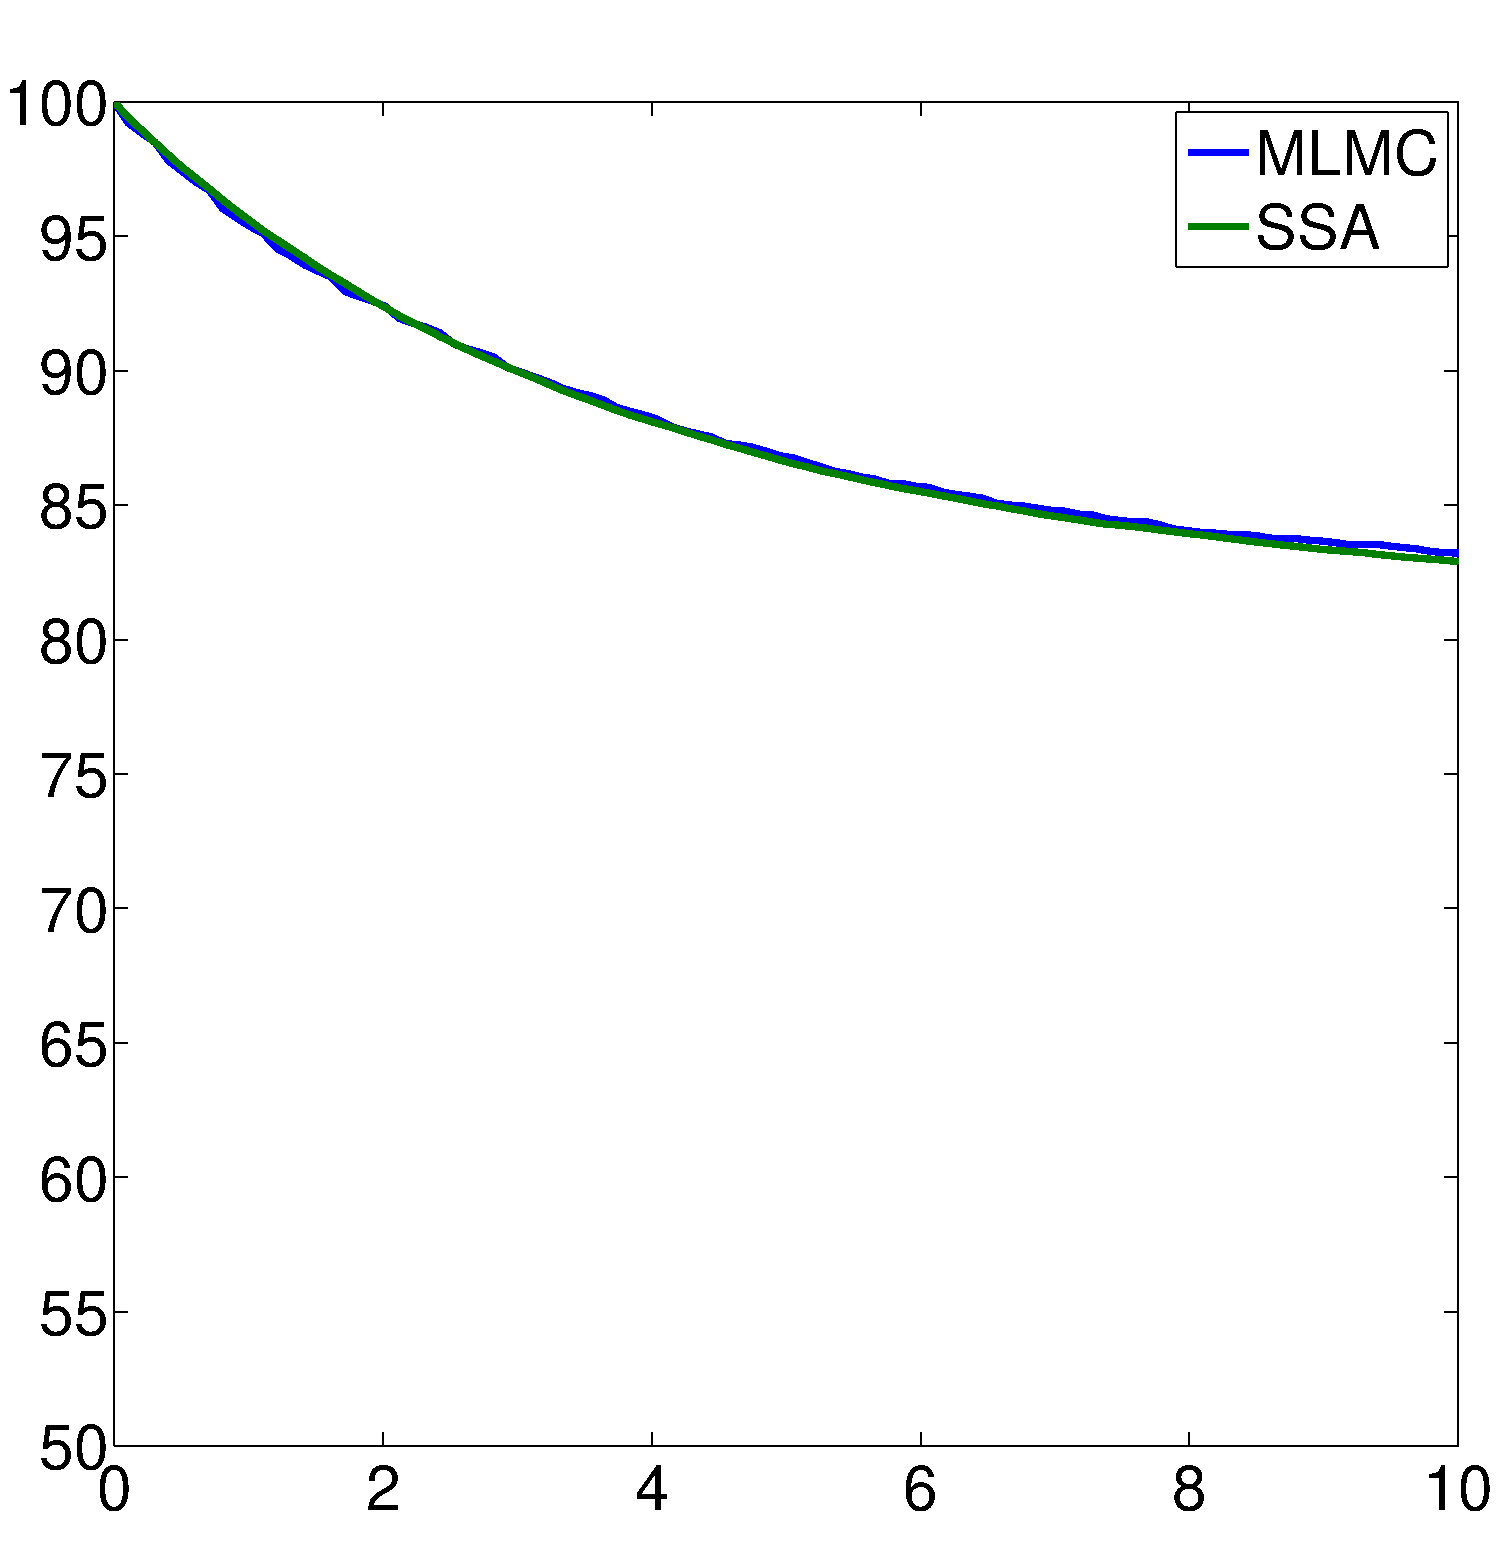
\includegraphics[width=0.5\textwidth]{figures/PC_c1_mlmc.pdf}
				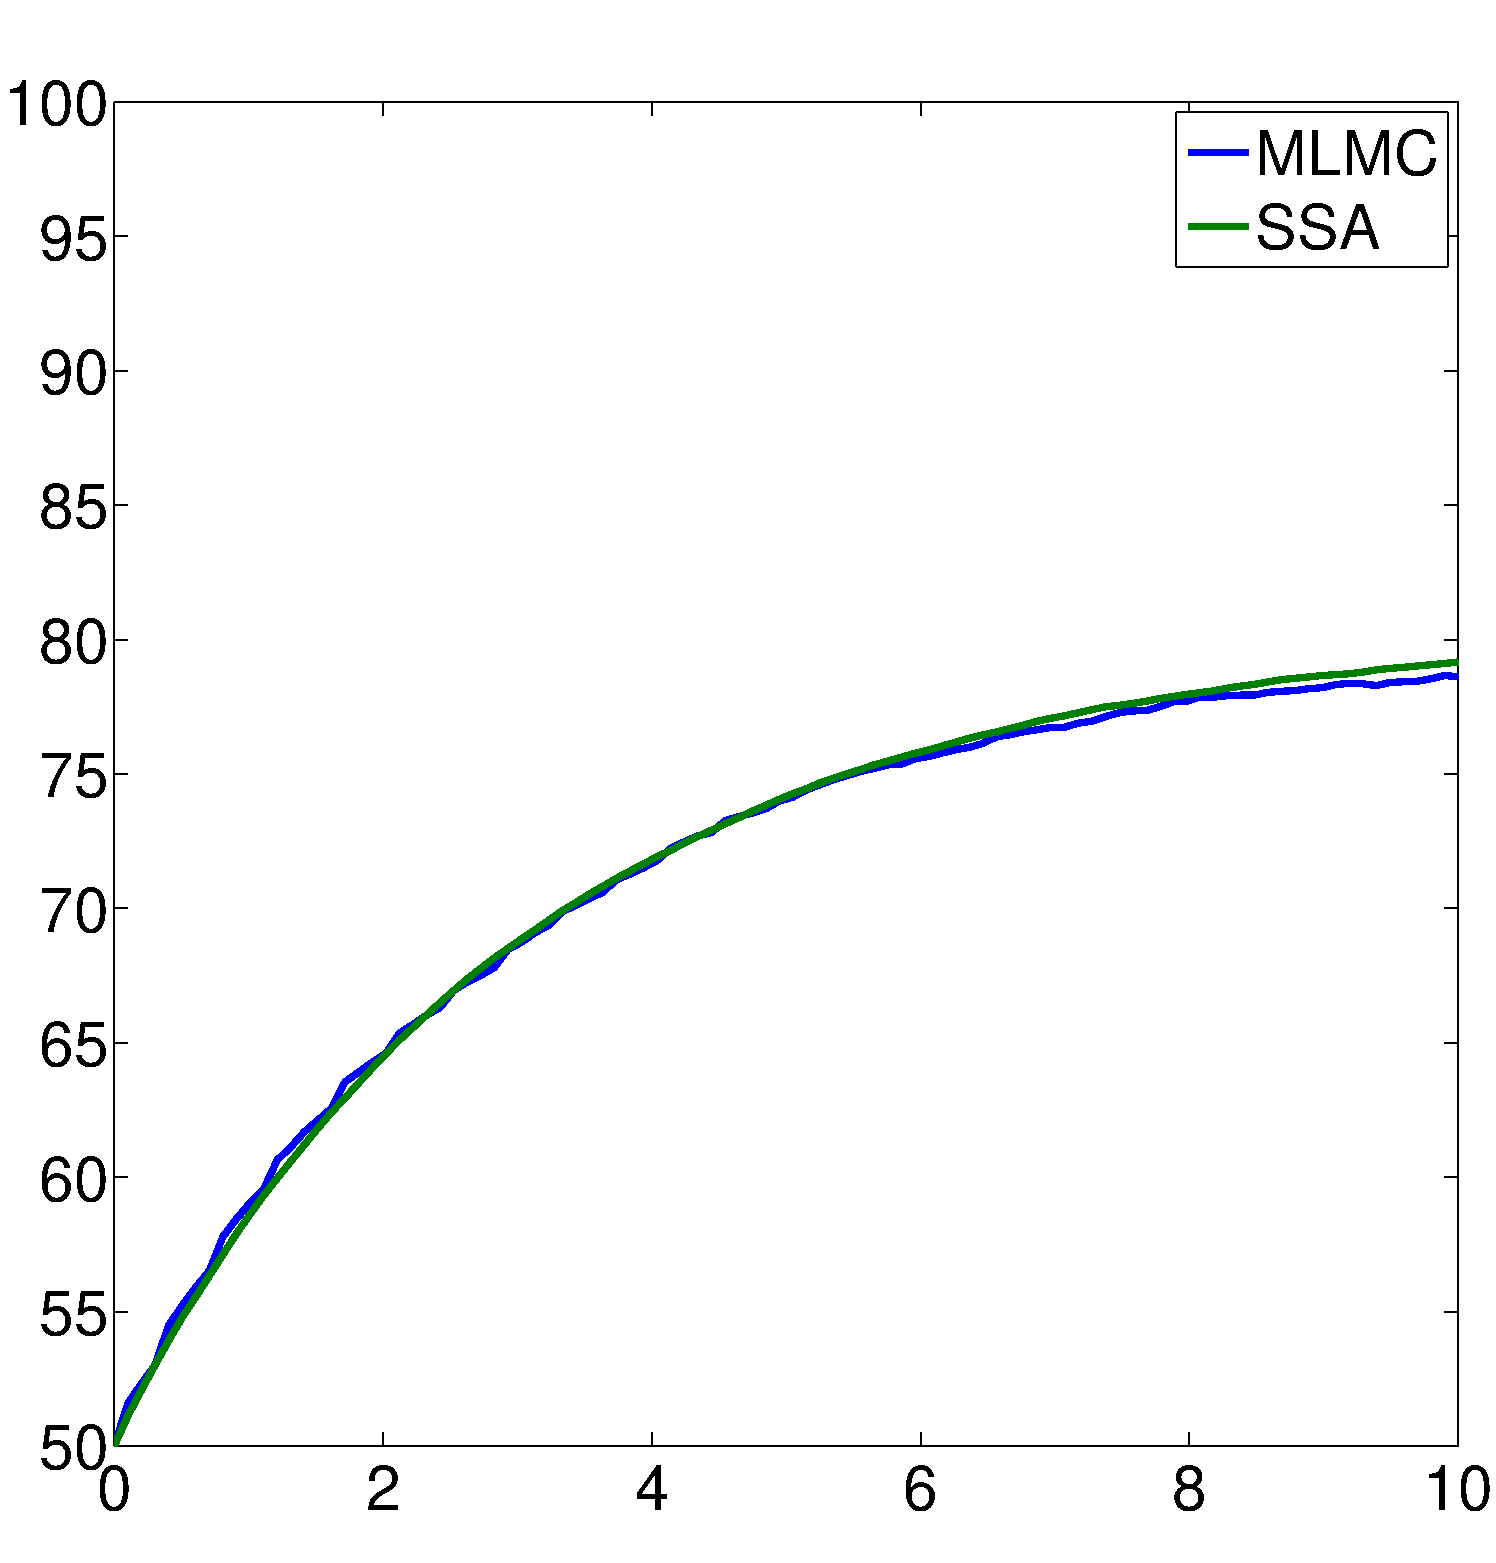
\includegraphics[width=0.5\textwidth]{figures/PC_c2_mlmc.pdf}
				}
			\centerline{
				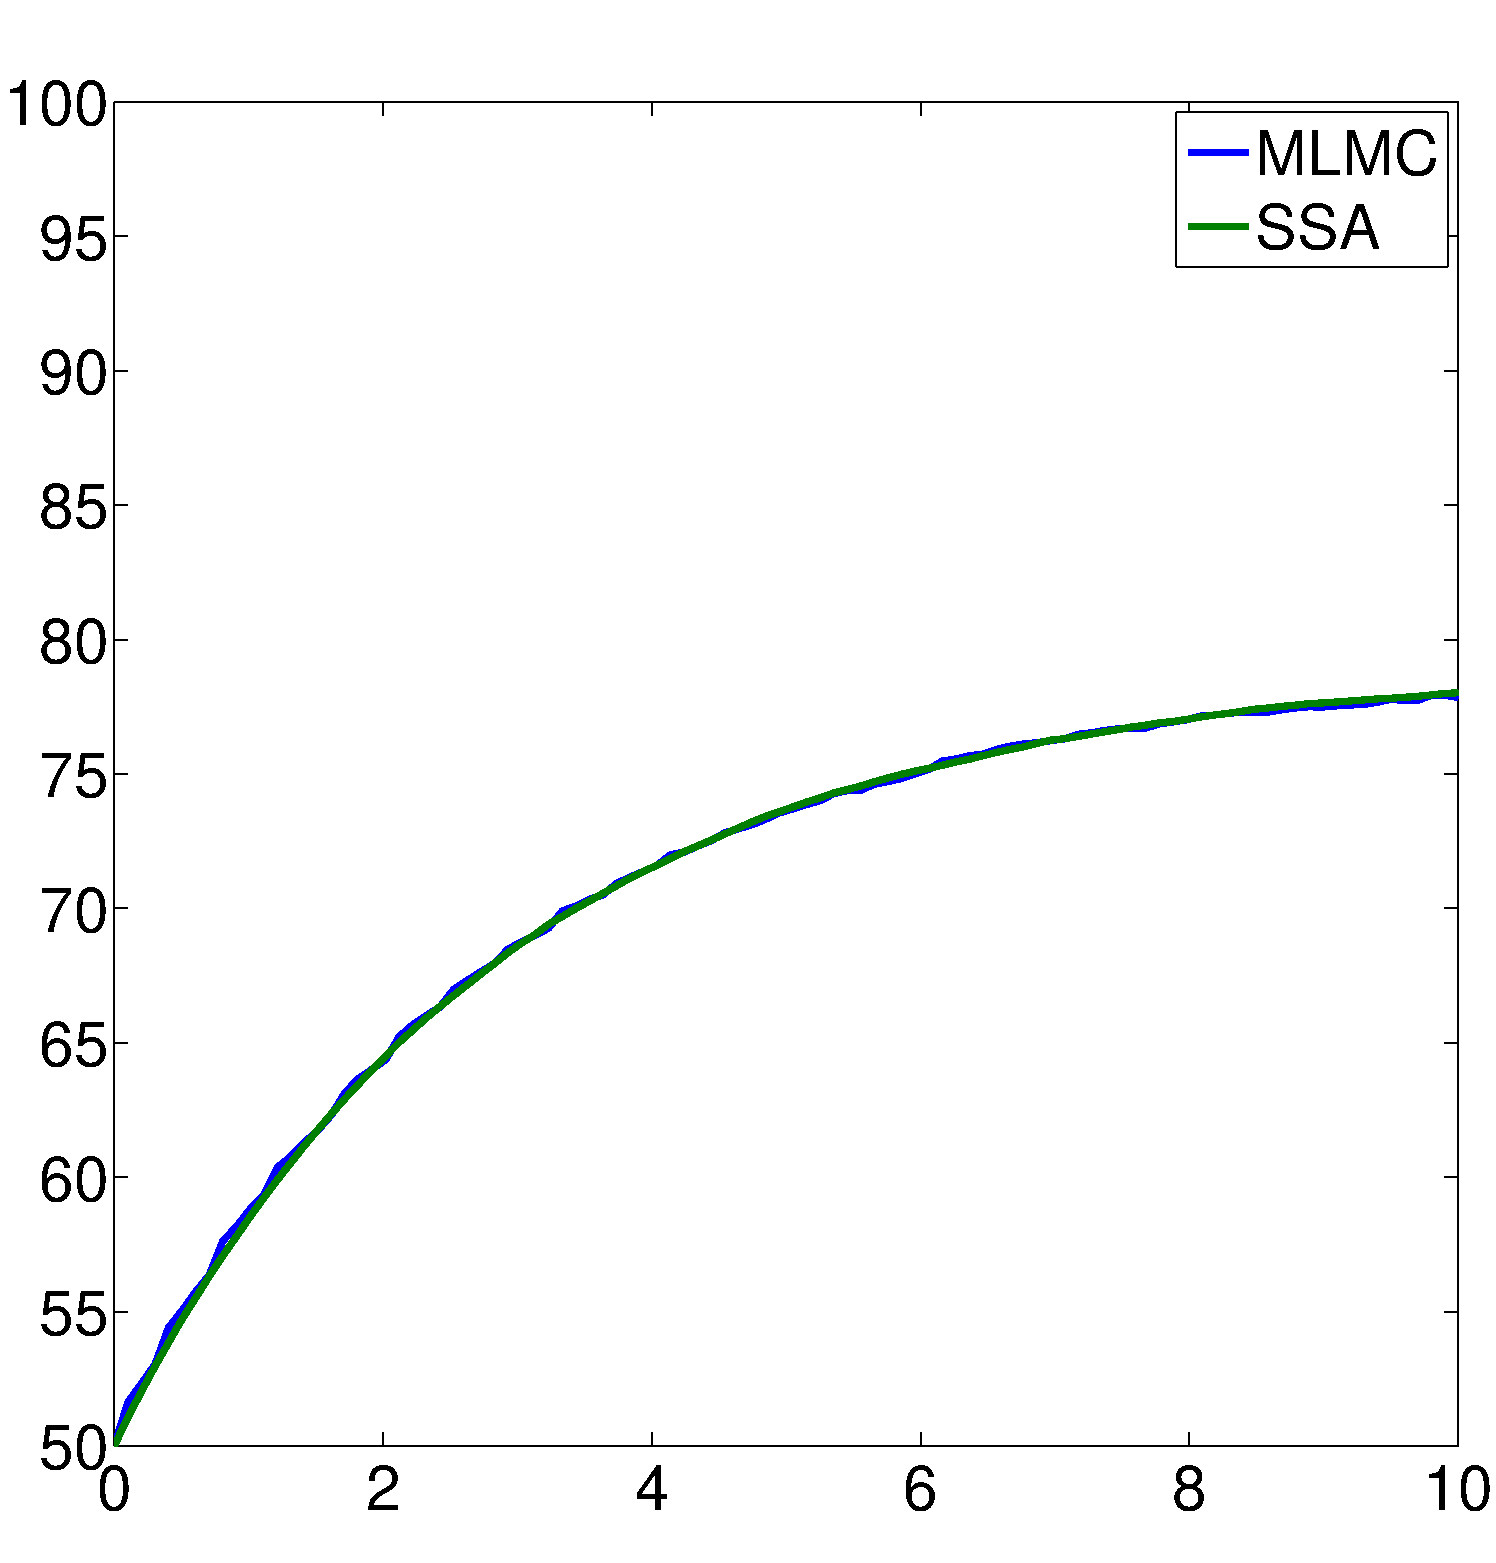
\includegraphics[width=0.5\textwidth]{figures/PC_o_mlmc.pdf}
				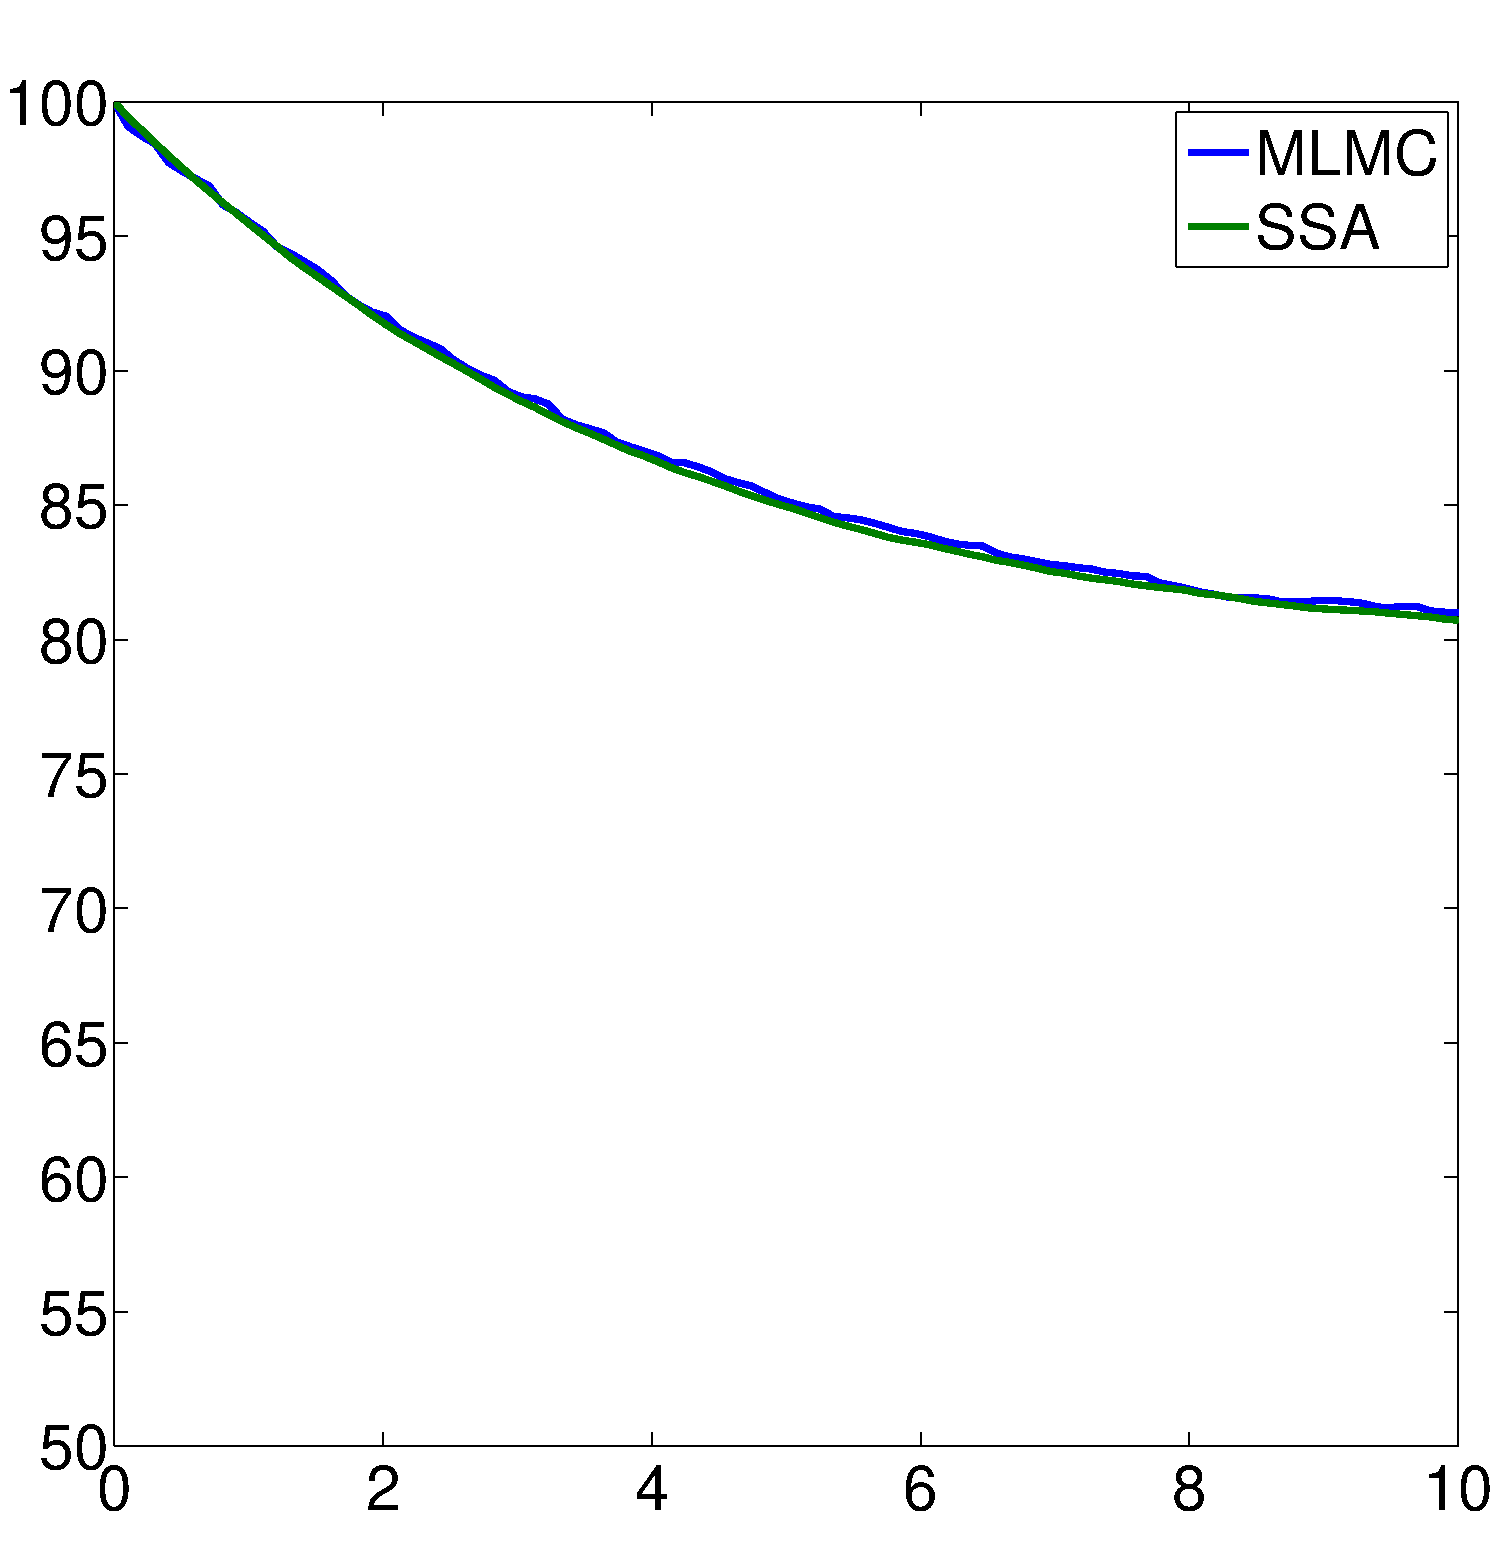
\includegraphics[width=0.5\textwidth]{figures/PC_i_mlmc.pdf}
				}
			\captionsetup{width=0.8\textwidth}
			\caption[Estimated average population values for species in Potassium Channel model using MLMC compared to 10,000 SSA trajectories over {$[0,10]$}]{The evolution of estimated average populations for species in Potassium Channel model computed using MLMC compared to average population values taken from 10,000 SSA trajectories. The results are shown for species $C_1$ (top left), $C_2$ (top right), $O$ (bottom left), and $I$ (bottom right). The vertical axis shows population amounts, while the horizontal axis shows simulation time. Integration was taken over $[0,10]$}
			\label{pc_mlmc}
			\end{figure}
			
			\noindent
			As with the previous models, the numerical results for the Potassium Channel model obtained with the MLMC method and with 10,000 SSA trajectories show a very good agreement. Moreover, the method MLMC strategy took about 2.92 seconds to complete, while the 10,000 SSA trajectories took about 42.65 seconds. This represents a 14.61 times speedup. The precise errors for the final population value are given in the Table \ref{pc_error}:

			\begin{table}[H]
			\centering
			\begin{tabular}{ >{$}l<{$} >{$}l<{$} >{$}l<{$}}
				\text{Species} 	& \text{Absolute error}	& \text{Relative error} \\
				\hline
				C_1 		& 3.20 \times 10^{-1}		& 3.58 \times 10^{-3} \\
				C_2			& 5.51 \times 10^{-1}		& 6.96 \times 10^{-3} \\
				C_3 		& 1.13 \times 10^{-1}		& 1.42 \times 10^{-3} \\
				O 	 		& 1.74 \times 10^{-1}		& 2.23 \times 10^{-3} \\
				I 	 		& 2.93 \times 10^{-1}		& 3.63 \times 10^{-3} \\
			\end{tabular}
			\captionsetup{width=0.8\textwidth}
			\caption{Errors for the estimated species populations in the Potassium Channel model using MLMC compared to 10,000 SSA trajectories}
			\label{pc_error}
			\end{table}


\chapter{Conclusion}

	We have now analyzed the reasons for the development and implementation of stochastic methods for simulating systems of biochemical reactions. Understanding these systems is crucial to the study of organism functionality and behaviour, and so methods that allow fast simulation and predictive capabilities are valuable to the field of Systems Biology, and by extension Biology as a whole. We have introduced the various traditional approaches for modelling biochemical systems, such as the Reaction Rate Equation, as well as the development of the Chemical Master Equation and in turn the Stochastic Simulation Algorithm, tau-leaping adaptations of Stochastic Simulation Algorithm, and the Chemical Langevin Equation. Further, we discussed the concept and implementation of the Multilevel Monte Carlo Tau-leaping method, showing that it approximates the solution to the Chemical Master Equation almost as accuratly as the gold standard of 10,000 SSA trajectories, but with much reduced computational complexity.\\
	\\
	Finally, we presented our software implementation making use of all these methods with a fair amount of capability, one which would allow anyone with an SBML file to obtain and plot data from systems of biochemical reactions with little knowledge of the mathematical techniques being used. This software is also scalable and parallalizable across either multiple CPUs or CPU cores, or a GPU, allowing for greatly reduced simulation times.\\ 
	\\
	A priority area with regards to future enhancements to the software would be to implement parallelization on a GPU using Nvidia's CUDA GPU programming language. The current GPU implementation, working purely in MATLAB, has its limitations, namely in terms of flexibility. It does not allow the recording of systems states throughout the simulation, nor currently provide an easy way to draw samples variable from a Poisson random variable. Additionally, many parameters must be hard-coded into the various function calls required, an obvious problem in dynamic software. Implementation using CUDA would solve nearly all of these problems with fewer or no workarounds, and given that it is a lower-level language, may also provide speed increases.\\
	\\
	Implementation of adaptive tau-leaping procedures would also be a very useful addition. Adaptive tau-leaping uses a variable step size that can sidestep some of the problems explicit constant step tau-leaping procedures suffer from, primarily some populations being driven negative. In addition, adaptive strategies would be important when dealing with stiff systems, as an adaptive step-size would lend itself particularly well to simulating systems containing multiple time scales.\\
	\\
	Moving forward, the modelling of systems of biochemical reaction will continue to be crucial to modern scientific progress. The importance of having the ability to predict and understand the behaviour of such systems cannot be overstated, and so it will likely be an area of relevance for some time to come.

\addcontentsline{toc}{chapter}{References}

\begin{thebibliography}{99}

\bibitem{mlmc_applications}
	D.F.~Anderson, D.J.~Higham, 2012, Multilevel Monte Carlo for continuous time Markov Chains with application to biochemical kinetics, {\it SIAM Multiscale Modeling and Simulation}, {\bf 10}, 146--179.

\bibitem{mlmc_complexity}
	D.F.~Anderson, D.J.~Higham, Y.~Sun, 2013, Complexity of Multilevel Monte Carlo Tau-Leaping, {\it arXiv:1310.2676v1 [math.NA]}.

\bibitem{libsbml}
	B.J.~Bornstein, S.M.~Keating, A.~Jouraku, M.~Hucka, 2008, LibSBML: An API Library for SBML, {\it Bioinformatics}, {\bf 24.6}, 880--881.

\bibitem{ssa_intro}
	D.T.~Gillespie, 1976, A general method for numerically simulating the stochastic time evolution of coupled chemical reactions, {\it Journal of Computational Physics}, {\bf 22}, 403--434.

\bibitem{gillespie_review}
	D.T.~Gillespie, 2007, Stochastic Simulation of Chemical Kinetics, {\it Annual Review of Physical Chemistry}, {\bf 58}, 35--55.

\bibitem{weiner_process}
	D.J.~Higham, 2001, An Algorithmic Introduction to Numerical Simulation of Stochastic Differential Equations, {\it SIAM Review}, {\bf 43.3}, 525--546.

\bibitem{sim_chem_reactions}
	D.J.~Higham, 2008, Modeling and Simulating Chemical Reactions, {\it SIAM Review}, {\bf 50.2}, 347--368.

\bibitem{schlogl}
	S.~Ilie, W.H.~Enright, K.R.~Jackson, 2009, Numerical solution of stochastic models of biochemical kinetics, {\it Canadian Applied Mathematics Quarterly}, {\bf 17.3}, 523--554.

\bibitem{sbml_toolbox}
	S.M.~Keating, B.J.~Bornstein, A.~Finney, M.~Hucka, 2006, SBMLToolbox: an SBML toolbox for MATLAB users, {\it Bioinformatics}, {\bf 22.10}, 1275--1277.

\bibitem{phage_bacteria}
	H.H.~McAdams, A.~Arkin, 1997, Stochastic mechanisms in gene expression, {\it Proceedings of the National Academy of Sciences of the United States of America}, {\bf 94}, 814-–819.

\bibitem{cme_intro}
	D.~McQuarrie, 1967, Stochastic approach to chemical kinetics, {\it Journal of Applied Probability}, {\bf 4}, 413--478.

\bibitem{chem_phys_models}
	B.~M\'{e}lyk\'{u}ti, K.~Burrage, K.C.~Zygalakis, 2010, Fast stochastic simulation of biochemical systems by alternative formulations of the chemical Langevin equation, {\it The Journal of Chemical Physics}, {\bf 132}, 164109.

\bibitem{stiffness}
	M.~Rathinam, L.R.~Petzold, Y.~Cao, D.T.~Gillespie, 2003, Stiffness, Stochastic Chemically Reacting Systems: The Implicit Tau-Leaping Method, {\it Journal of Chemical Physics}, {\bf 119}, 12784.

\bibitem{sys_bio_intro}
	D.J.~Wilkinson, 2009, Stochastic modelling for quantitative description of heterogeneous biological systems, {\it Nature Reviews Genetics}, {\bf 10.2}, 122--133.

\end{thebibliography}

\begin{appendices}

	\chapter{Source Code}

	Please note the source code can be downloaded in its entirety, including with the required libraries, from \url{https://github.com/dbarrows/mars}, though it may not yet be available for download at the time of publication. It should be noted that the source code download also contains the SBMLToolbox and libSBML, libraries and tools required to interact with SBML files. The source code included in this appendix does \textit{not} include these files, it contains only the original work of the author, which is limited to components that build on top of these additional libraries and tools.

	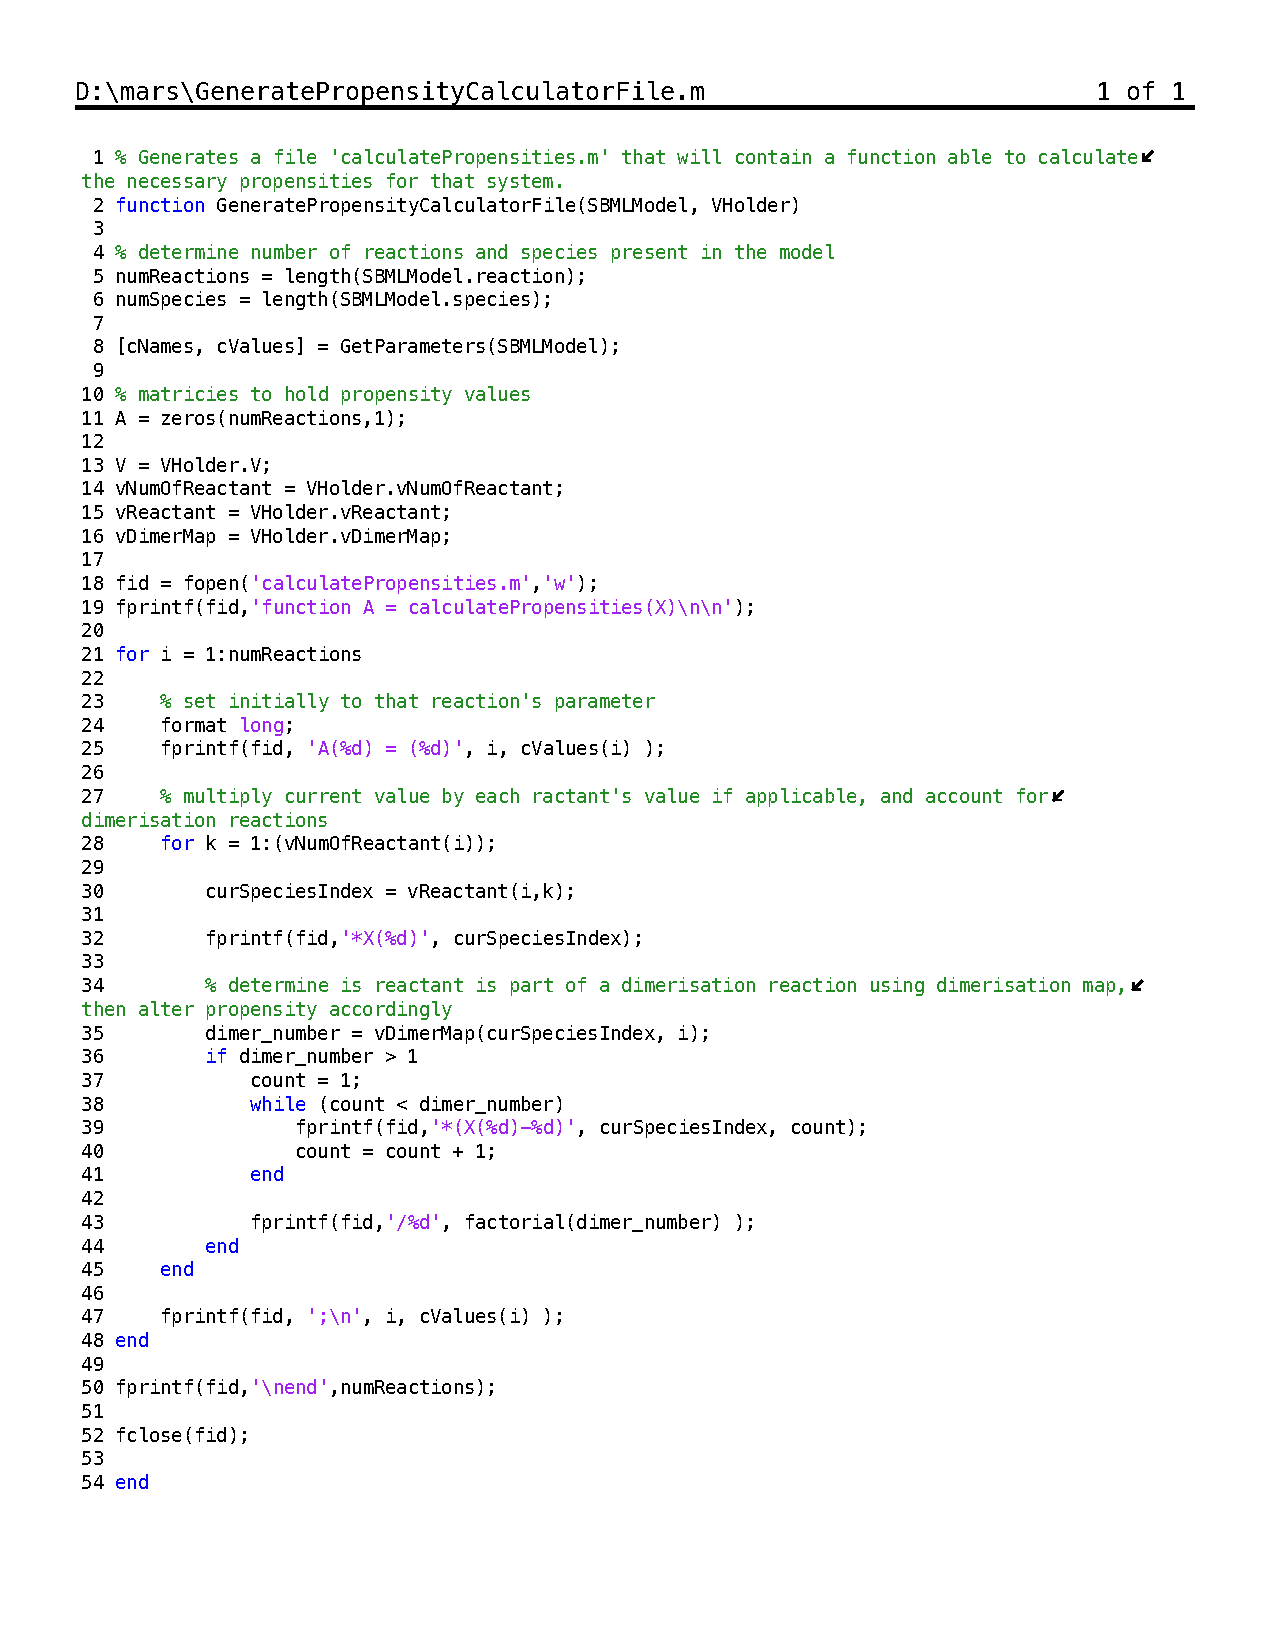
\includepdf[pages=-]{MARS-source.pdf}

\end{appendices}


\end{document}












